%%%%%%%%%%%%%%%%%%%%%%%%%%%%%%%%%%%%%%%%%%%%%%%%%%%%
\chapter{Inductance Characterization}\label{Appendix: AA}
\section{Inductance Estimation Table}

\begin{table}[ht]
\begin{center}
 \setlength{\tabcolsep}{12pt}
\begin{tabular}{cccccccc}

\noalign{\global\arrayrulewidth1pt}
\hline
% \noalign{\global\arrayrulewidth0.4pt}
$D/l$ 	& $K$ 	& 	$D/l$ 	& $K$ 	& 	$D/l$ 	& $K$ 	& 	$D/l$ 	& $K$\\
\noalign{\global\arrayrulewidth0.5pt}
\hline
% \noalign{\global\arrayrulewidth0.4pt}

0.02  & 0.1957 	& 	0.32 	& 	2.769 	& 	0.80 	&	5.803 	& 	2.20 	& 	10.93\\ %\hline 
0.04  & 0.3882 	& 	0.34 	& 	2.919 	& 	0.85  	& 	6.063 	& 	2.40 	& 	11.41\\ %\hline 
0.06  & 0.5776 	& 	0.36 	& 	3.067 	& 	0.90 	& 	6.171 	& 	2.60 	& 	12.01\\ %\hline 
0.08  & 0.7643 	& 	0.38 	& 	3.212 	& 	0.95    & 	6.559 	& 	2.80 	& 	12.30\\ %\hline 
0.10  & 0.9465 	& 	0.40  	& 	3.355 	& 	1.00 	& 	6.795 	& 	3.00 	& 	12.71\\ %\hline
0.12  & 1.126 	& 	0.42 	& 	3.497 	& 	1.10 	&	7.244 	& 	3.50 	& 	13.63\\ %\hline 
0.14  & 1.303 	& 	0.44 	& 	3.635 	& 	1.20  	& 	7.670 	& 	4.00 	& 	14.43\\ %\hline 
0.16  & 1.477 	& 	0.46 	& 	3.771 	& 	1.30 	& 	8.060 	& 	4.50 	& 	15.14\\ %\hline 
0.18  & 1.648 	& 	0.48 	& 	3.905 	& 	1.40    & 	8.453 	& 	5.00 	& 	15.78\\ %\hline 
0.20  & 1.817 	& 	0.50  	& 	4.039 	& 	1.50 	& 	8.811 	& 	6.00 	& 	16.90\\ %\hline
0.22  & 1.982 	& 	0.55  	& 	4.358 	& 	1.60 	& 	9.154 	& 	7.00 	& 	17.85\\ %\hline
0.24  & 2.144 	& 	0.60 	& 	4.668 	& 	1.70 	&	9.480 	& 	8.00 	& 	18.68\\ %\hline 
0.26  & 2.305 	& 	0.65 	& 	4.969 	& 	1.80  	& 	9.569 	& 	9.00 	& 	19.41\\ %\hline 
0.28  & 2.406 	& 	0.70 	& 	5.256 	& 	1.90 	& 	10.09 	& 	10.00 	& 	20.07\\ %\hline 
0.30  & 2.616 	& 	0.75 	& 	5.535 	& 	2.00    & 	10.37 	& 	12.00 	& 	21.21\\ 

\noalign{\global\arrayrulewidth1pt}
\hline 

\end{tabular}
\caption{Coefficient K}
\label{T:K}
\end{center}
\end{table}

\section{Equivalent coil impedance} \label{AppendixSection: impedance}

The impedance of the coil is defined as follows:

\begin{equation}
Z = (j\omega{C_{par}}+\frac{1}{R+j\omega{L}})^{-1}
\end{equation}

by developing the equation, this impedance can be separated into a real and an imaginary term,

\begin{equation}
\Re{Z}=\frac{R}{(\omega{R}C_{par})^2+(1-\omega^2LC_{par})^2}
\end{equation}

\begin{equation}
\Im{Z}=\frac{\omega{L}-\omega{R^2}C-\omega^3L^2C_{par}}{(1-\omega^2LC_{par})^2+(\omega{R}C_{par})^2}
\end{equation}





%%%%%%%%%%%%%%%%%%%%%%%%%%%%%%%%%%%%%%%%%%%%%%%%%%%%
%%%%%%%%%%%%%%%%%%%%%%%%%%%%%%%%%%%%%%%%%%%%%%%%%%%%
%%%%%%%%%%%%%%%%%%%%%%%%%%%%%%%%%%%%%%%%%%%%%%%%%%%%
%%%%%%%%%%%%%%%%%%%%%%%%%%%%%%%%%%%%%%%%%%%%%%%%%%%%
\chapter{Model equations} \label{Appendix: A}
\section{Secondary capacitor in series} \label{sec:secondaryS}

By adding a capacitor in series in the secondary side, there is a notable different expressions for $Z_2$ and $Z_R$. $Z_R$ has a capacitive reactance that prevents to transfer the maximum power to the secondary. 

\begin{equation}
Z_2 = R_2+R_L+j\omega{L_2}-j\frac{1}{\omega{C_2}}
\end{equation}

\begin{equation}
Z_R = \frac{(R_2+R_L)\omega^{4}L_2^{2}C_2^{2}}{(R_2+R_L)^{2}\omega^{2}C_2^{2}+(\omega^{2}L_2C_2-1)^{2}}-j\frac{\omega^{3}M^{2}C_2(\omega^{2}L_2C_2-1)}{(R_2+R_L)^{2}\omega^{2}C_2^{2}+(\omega^{2}L_2C_2-1)^{2}}
\end{equation}
\\

When the operating frequency is the resonance frequency $\omega_0$, obtained by using the Equation \ref{Eq:naturalFrequency}, the imaginary part of $Z_R$, that is a source of additional losses, is canceled and it will only remain its real part. Thus, the power transferred to the receiving circuit becomes only active power, and as a result, the consumable power. A simpler equation of $Z_R$ is obtained which only depends on $R_L$ if the distance is fixed, allowing to match this impedance with the primary circuit.

\begin{equation}
Z_R = \frac{\omega_0^{2}M^{2}}{R_2+R_L}
\end{equation}

\section{Secondary capacitor in parallel}\label{sec:secondaryP}

The same steps as above are followed for obtaining the impedances $Z_2$ and $Z_R$ when the secondary capacitor is placed in parallel: 

\begin{equation}
Z_2 = R_2+j\omega{L_2}+\frac{1}{\frac{1}{R_L}+j\omega{C_2}} 
\end{equation}

\begin{equation} \label{eq:SecParZR}
\begin{aligned}
Z_R = \frac{\omega^{2}M^{2}(1+\omega^{2}L_2^{2}R_L^{2})(R_2+R_L+\omega^{2}L_2C_2R_L)}{(R_2+R_L+\omega^{2}L_2C_2R_L)^{2}+(\omega L_2-\omega C_2R_LR_2-\omega C_2R_L^{2})^{2}} \\[10pt]
-j\frac{\omega^{2}M^{2}(1+\omega^{2}L_2^{2}R_L^{2})(\omega L_2-\omega C_2R_LR_2-\omega C_2R_L^{2})}{(R_2+R_L+\omega^{2}L_2C_2R_L)^{2}+(\omega L_2-\omega C_2R_LR_2-\omega C_2R_L^{2})^{2}}
\end{aligned}
\end{equation}
\\

In this case, $Z_R$ shows also a capacitive reactance that has to be avoided to transfer the maximum power. If we work at resonance frequency $\omega_0$, this reactance still remains:

\begin{equation}
\begin{aligned}
Z_R = \frac{\omega_0^{2}M^{2}(1+\omega_0^{2}L_2^{2}R_L^{2})(R_2+2R_L)}{(R_2+2R_L)^{2}+(\omega_0 L_2-\frac{R_LR_2}{\omega_0L_2}-\frac{R_L^{2}}{\omega_0L_2})^{2}} \\[10pt]
-j\frac{\omega_0^{2}M^{2}(1+\omega_0^{2}L_2^{2}R_L^{2})(\omega_0 L_2-\frac{R_LR_2}{\omega_0L_2}-\frac{R_L^{2}}{\omega_0L_2})}{(R_2+2R_L)^{2}+(\omega_0 L_2-\frac{R_LR_2}{\omega_0L_2}-\frac{R_L^{2}}{\omega_0L_2})^{2}}
\end{aligned}
\end{equation}
\\

The solution is to select a capacitance value able to delete the imaginary part of the Equation \ref{eq:SecParZR}. A drawback of this option is the dependence of this capacitor on the load and that the system will not oscillate at the resonance frequency in the secondary side:

\begin{equation} \label{Eq:differentCapacitor}
C_2 = \frac{L_2}{R_L}\frac{1}{(R_2+R_L)}
\end{equation}

\section{Primary capacitor in series}\label{sec:primaryS}

The goal of the secondary capacitor was to cancel the imaginary part of the reflected impedance and the primary capacitor had a similar objective, that is to cancel the inductance of the coil. In a series compensated primary that works at resonance frequency, the imaginary part is fully deleted. The total impedance seen by the voltage source $Z_{eq}$ has the following expression:

\begin{equation}
Z_{eq} = R_1+j\omega{L_1}-j\frac{1}{\omega{C_1}}+Z_R
\end{equation}

At resonance frequency $\omega_0$, the imaginary part of $Z_{eq}$ is canceled and this impedance becomes dependent only on the secondary circuit expressed in $Z_R$.

\begin{equation}
Z_{eq} = R_1+Z_R
\end{equation}

\section{Primary capacitor in parallel}\label{sec:primaryP}

When the primary capacitor is placed in parallel, the total impedance $Z_{eq}$ is given by:

\begin{equation*}
Z_{eq} = \frac{1}{j\omega{C_1}+\frac{1}{R_1+j\omega{L_1}+Z_R}} 
\end{equation*}

\begin{equation} \label{eq:PriParZeq}
Z_{eq} = \frac{R_1+Z_R}{(1-\omega^2C_1L_1)^2+\omega^2C_1^2(R_1+Z_R)^2}-j\frac{\omega{C_1}(R_1+Z_R)^2-\omega{L_1}(1-\omega^2C_1L_1)}{(1-\omega^2C_1L_1)^2+\omega^2C_1^2(R_1+Z_R)^2}
\end{equation}

When the operating frequency is the resonance frequency $\omega_0$, $Z_{eq}$ becomes as it is shown below.

\begin{equation}
Z_{eq} = \frac{\omega_0^2L_1^4}{R_1+Z_R}-j\omega_0L_1^3 
\end{equation}

Note that as in case of the secondary capacitor in parallel, the reactance still remains and the solution could also be to select a capacitor that cancels the imaginary part of the Equation \ref{eq:PriParZeq}.

\begin{equation} \label{Eq:differentCapacitor2}
C_1 = \frac{L_1}{(R_1+Z_R)^2+\omega_0^2L_1^2}
\end{equation} 

Now, this capacitor depends on the frequency and the reflected impedance which is dependent on the topology used in the secondary, the mutual inductance and the load resistance.


%%%%%%%%%%%%%%%%%%%%%%%%%%%%%%%%%%%%%%%%%%%%%%%%%%%%
%%%%%%%%%%%%%%%%%%%%%%%%%%%%%%%%%%%%%%%%%%%%%%%%%%%%
%%%%%%%%%%%%%%%%%%%%%%%%%%%%%%%%%%%%%%%%%%%%%%%%%%%%







%%%%%%%%%%%%%%%%%%%%%%%%%%%%%%%%%%%%%%%%%%%%%%%%%%%%
\chapter{Coils Experimental Results}
\section{Inductance and Resistance}\label{sec:RL}

\begin{figure}[htb]
\centering
\begin{subfigmatrix}{2} 
\subfigure[Model A transmitter]
	{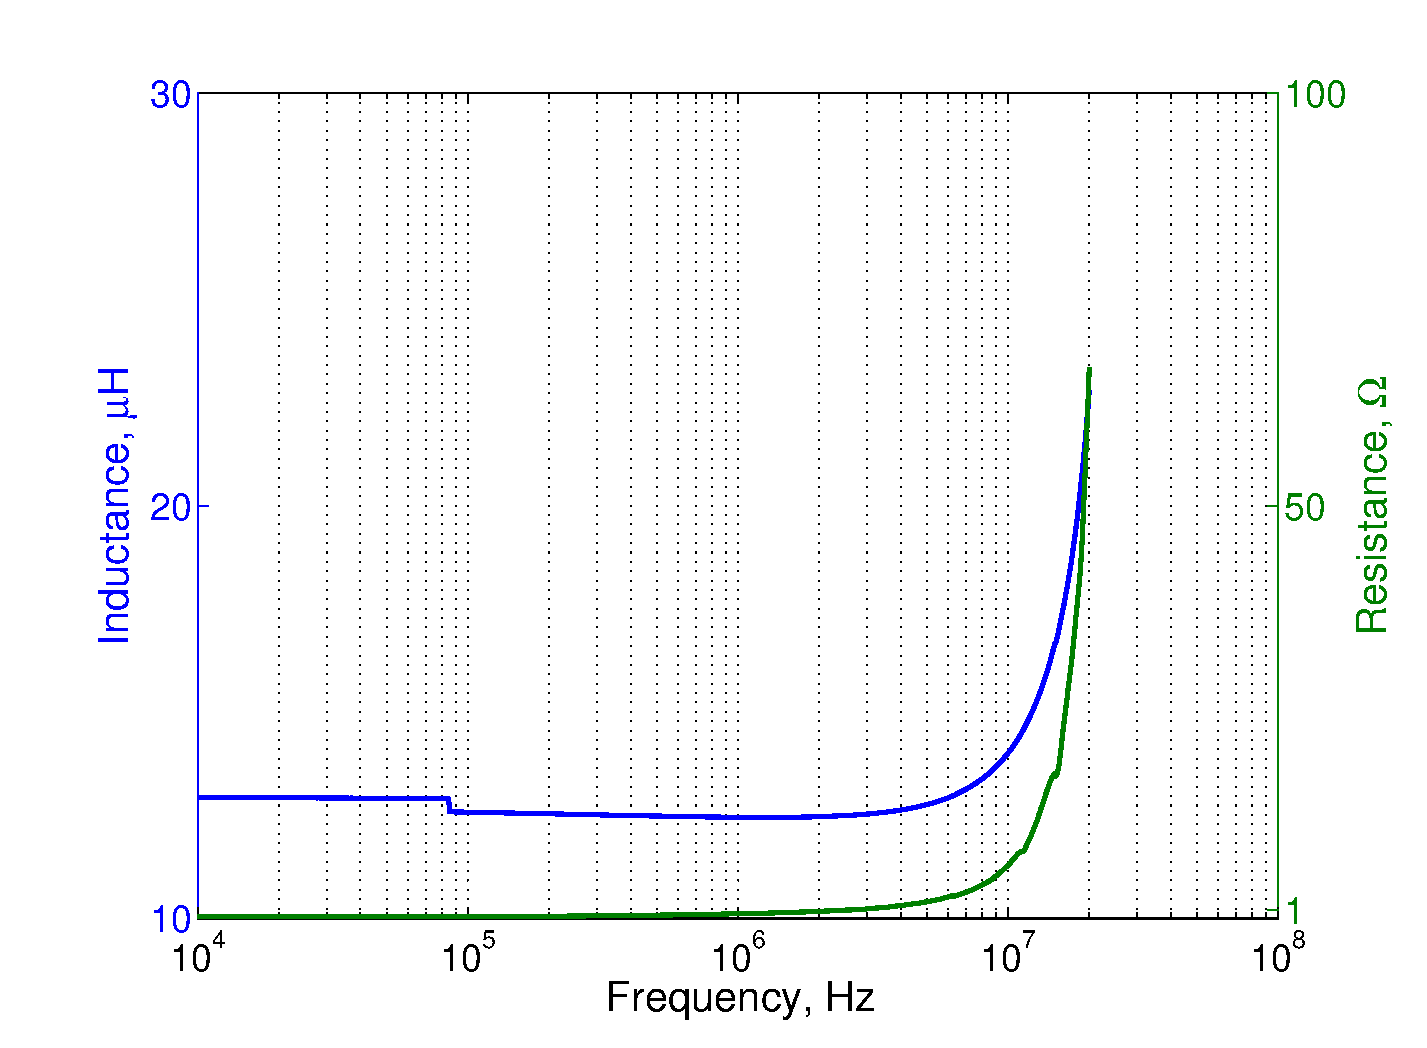
\includegraphics{./images/atx}\label{F:LRatx}} 
\subfigure[Model A receiver]
	{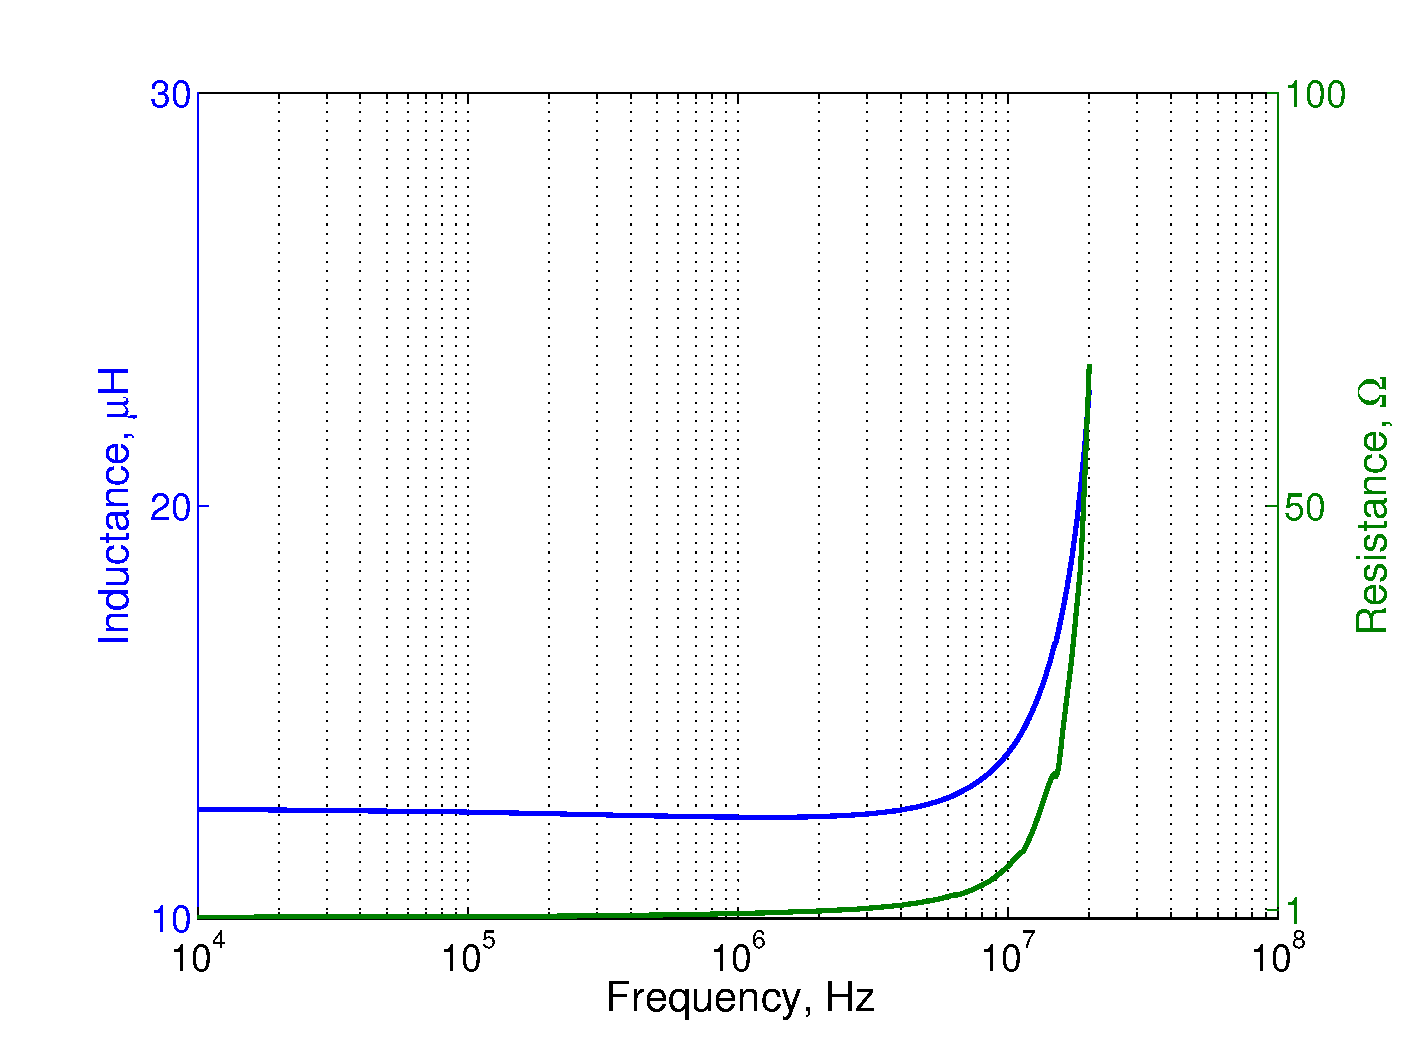
\includegraphics{./images/arx}\label{F:LRarx}}
\subfigure[Model B transmitter] 
	{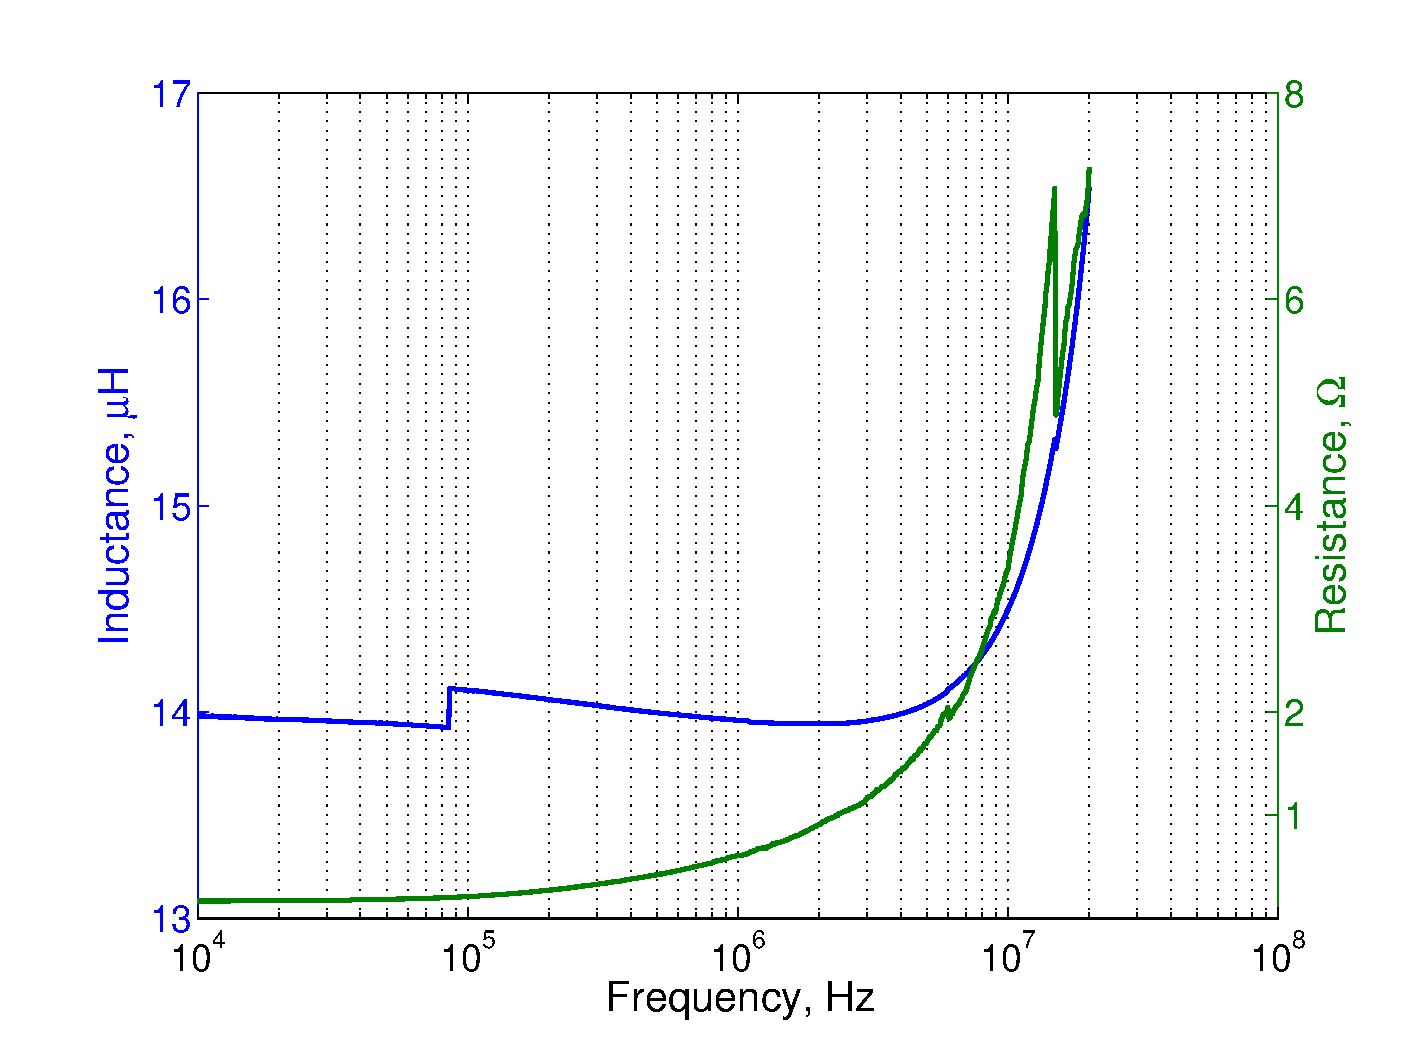
\includegraphics{./images/btx}\label{F:LRbtx}} 
\subfigure[Model B receiver]
	{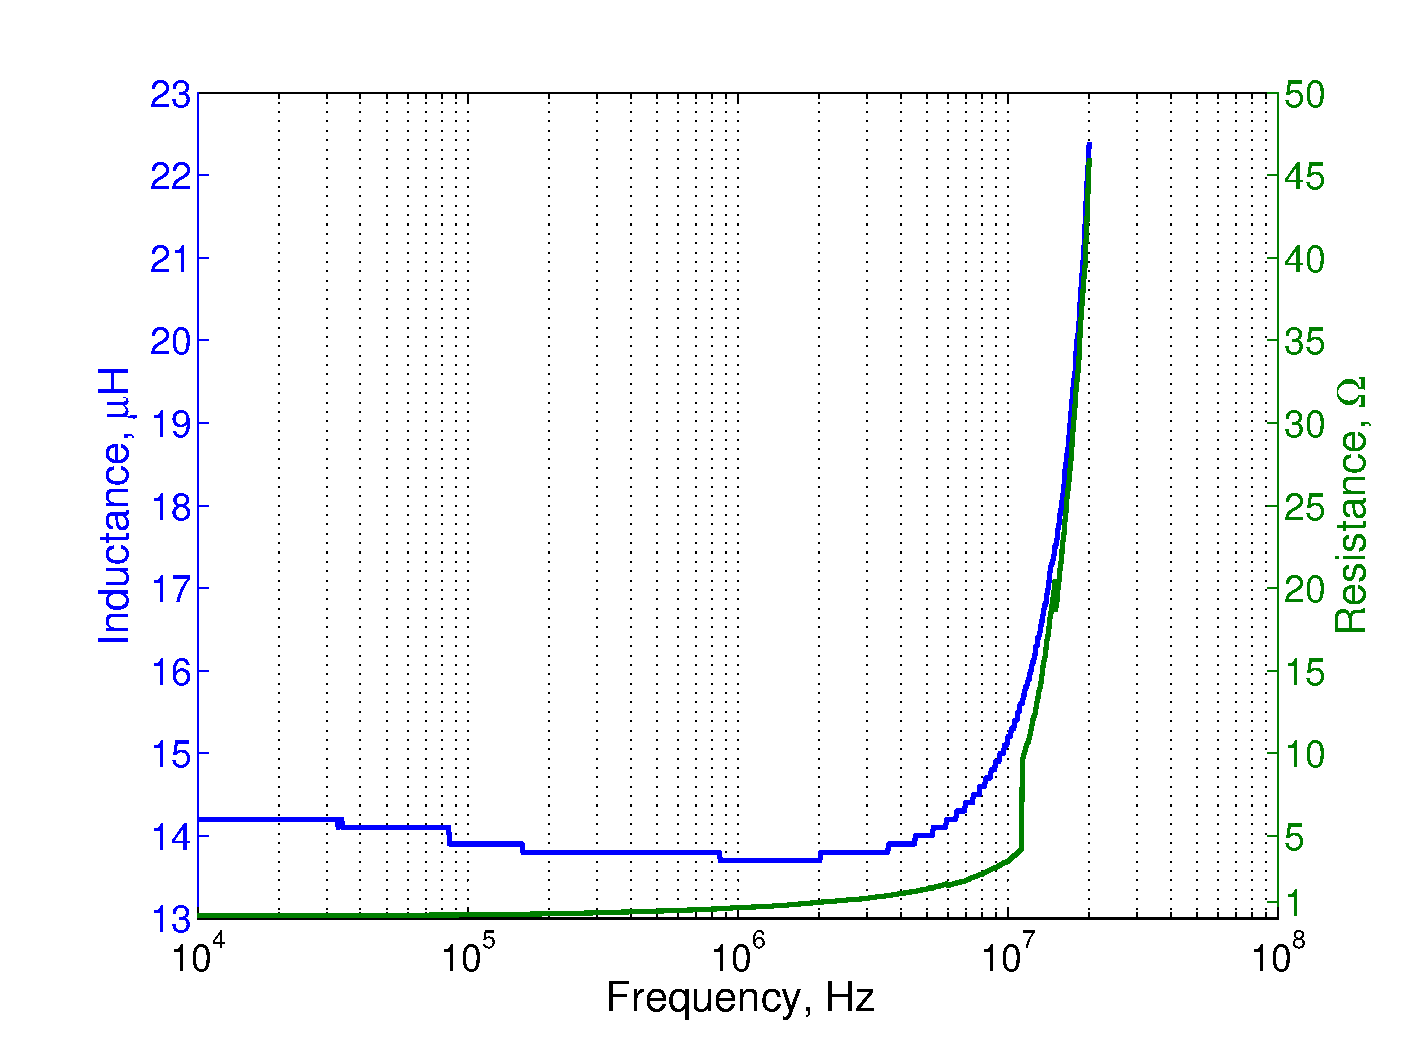
\includegraphics{./images/brx}\label{F:LRbrx}}
\subfigure[Model C transmitter]
	{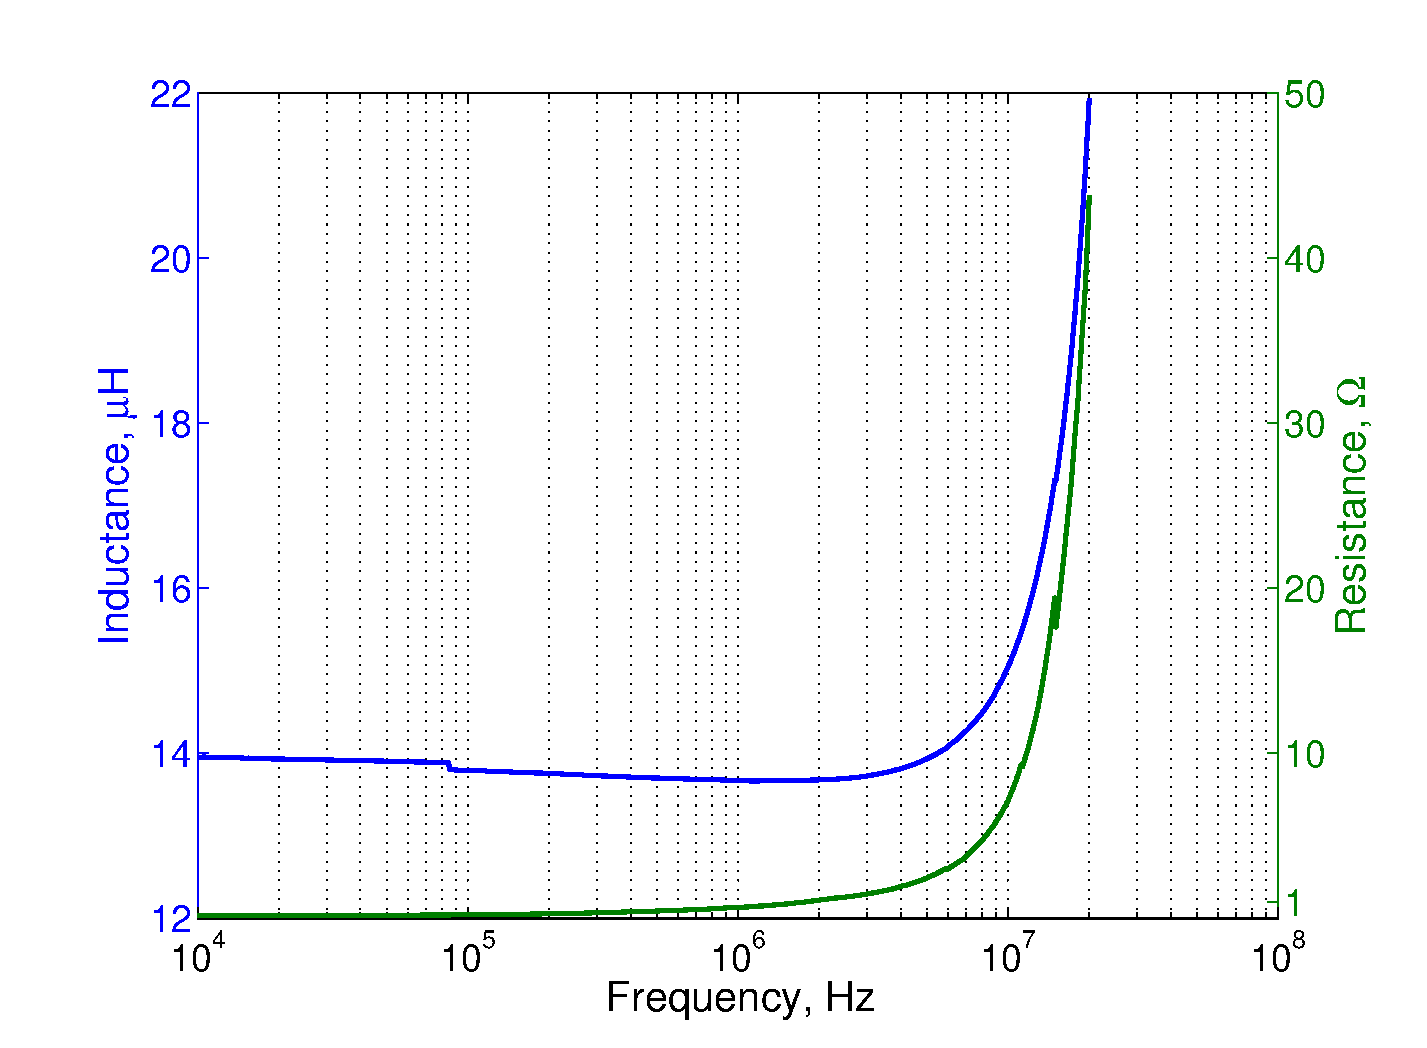
\includegraphics{./images/ctx}\label{F:LRctx}} 
\subfigure[Model C receiver]
	{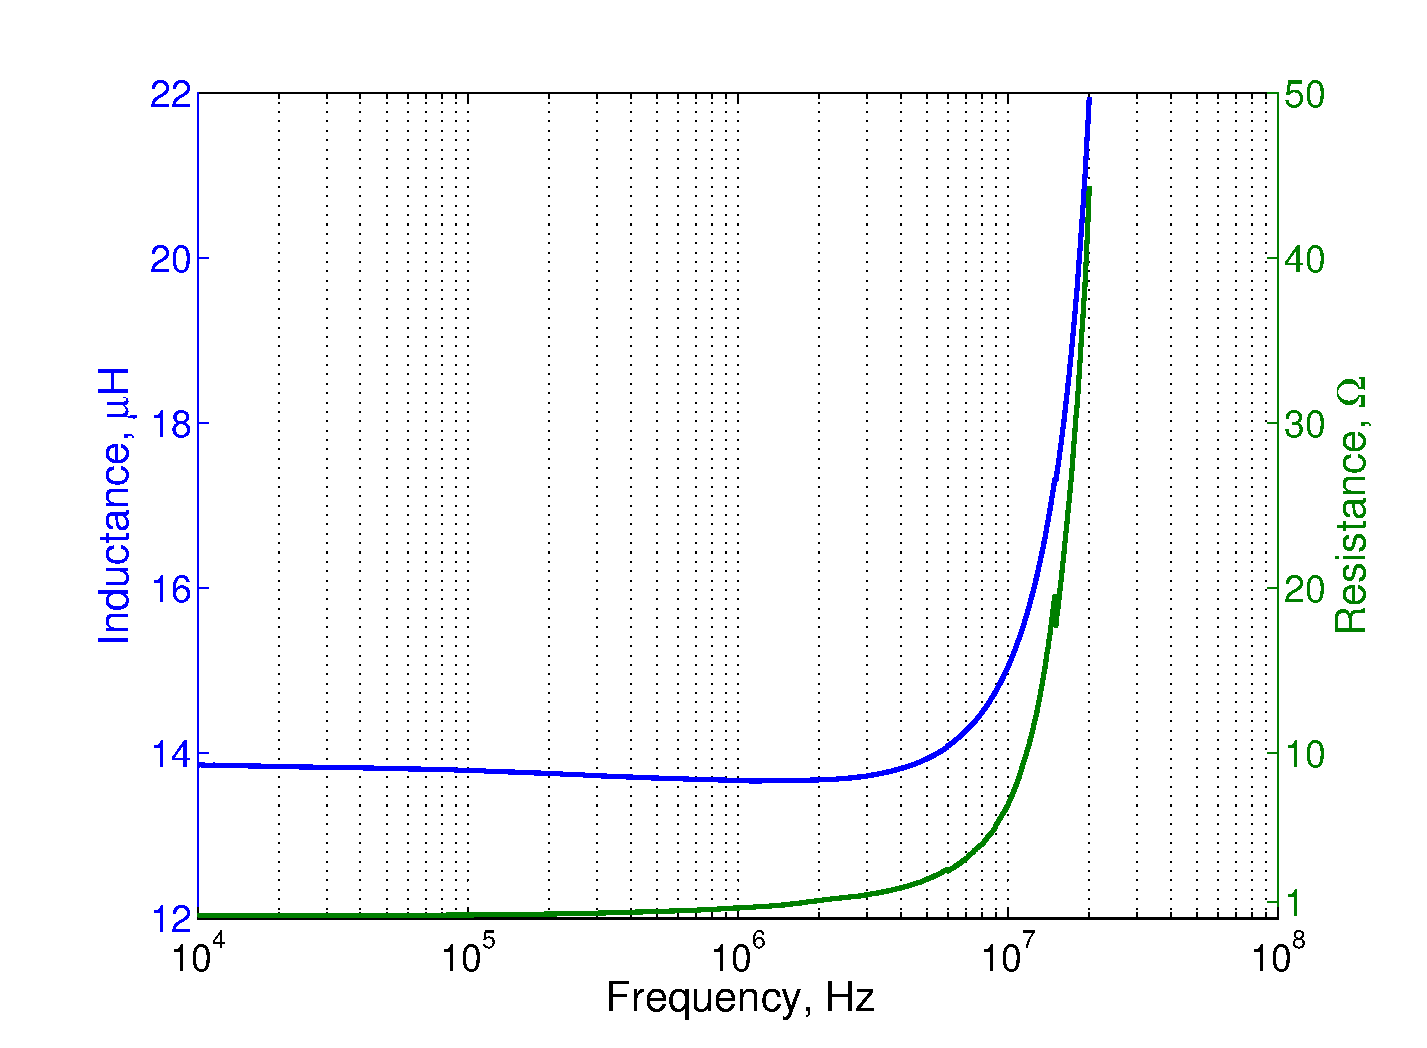
\includegraphics{./images/crx}\label{F:LRcrx}}
\end{subfigmatrix}
\end{figure}

\begin{figure}[H]
\centering
\begin{subfigmatrix}{2} 
\subfigure[Model D1] 
	{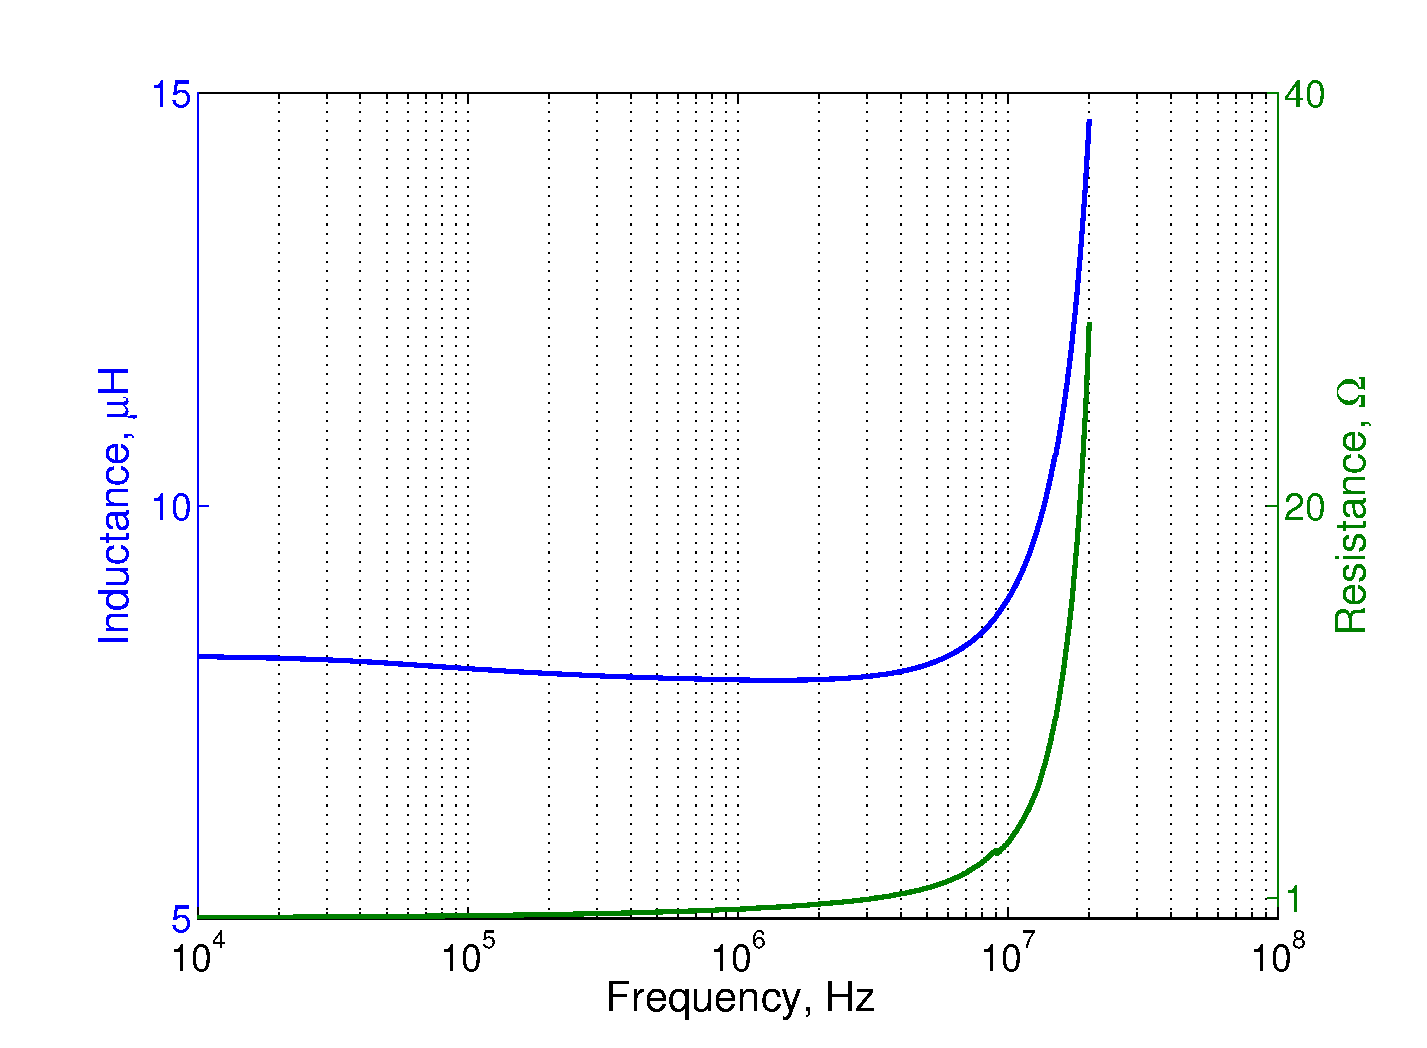
\includegraphics{./images/d1}\label{F:LRd1}} 
\subfigure[Model D2]
	{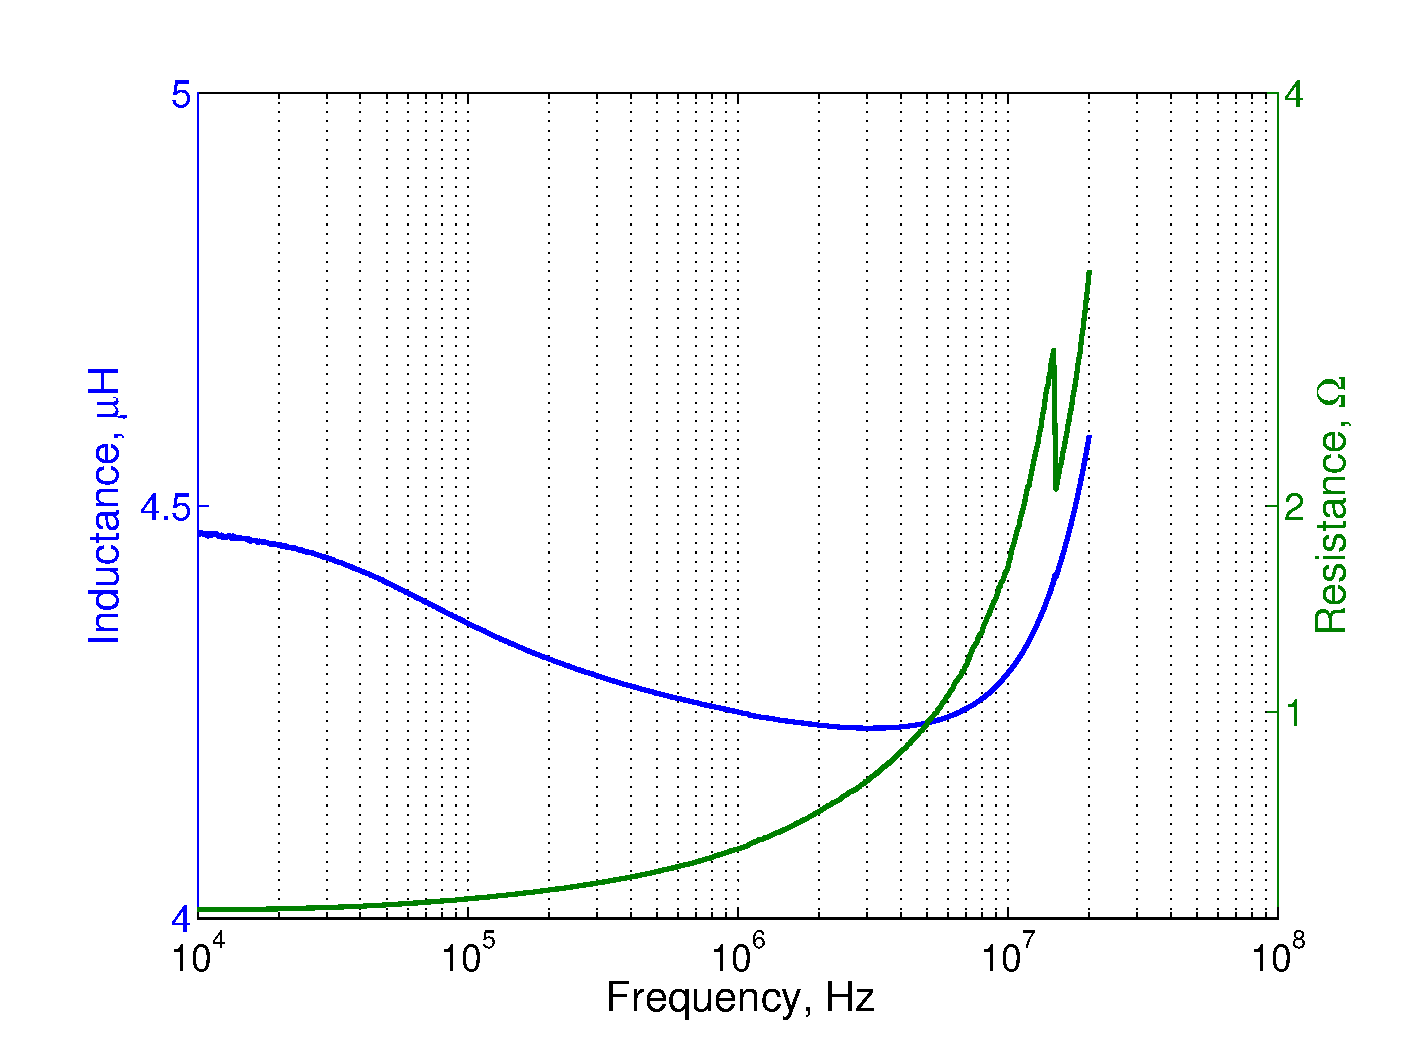
\includegraphics{./images/d2}\label{F:LRd2}}
\end{subfigmatrix}
\caption{Inductance and resistance w.r.t. frequency}
\label{F:LRvsF}
\end{figure}


\section{Quality Factor}

\begin{figure}[htb]
\centering
\includegraphics[width=1\textwidth]{./images/QFactorall}
\caption{Experimental quality factor}
\label{F:QFactorAll}
\end{figure}






%%%%%%%%%%%%%%%%%%%%%%%%%%%%%%%%%%%%%%%%%%%%%%%%%%%%
%%%%%%%%%%%%%%%%%%%%%%%%%%%%%%%%%%%%%%%%%%%%%%%%%%%%
\chapter{Circuit Schematics}

\section{Voltage Regulator}\label{Appendix: DC-DC}

% \begin{figure}[htb]
% 	\begin{center}
% 		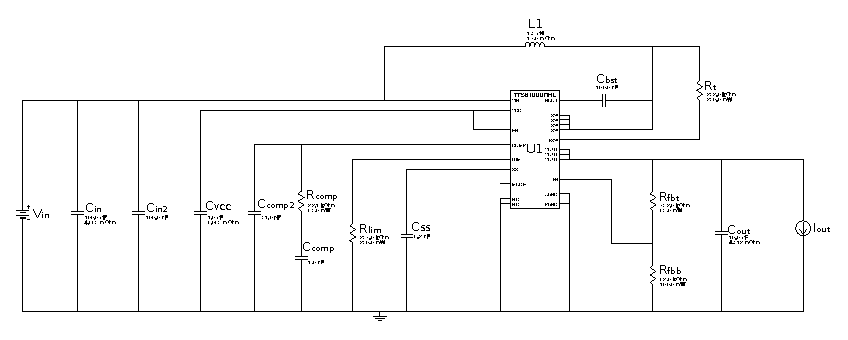
\includegraphics[width=1.05\textwidth]{./images/TPS61088}
% 	\caption{TPS61088 design circuit}
% 	\end{center}
% \end{figure}

\begin{figure}[htb]
	\begin{center}
		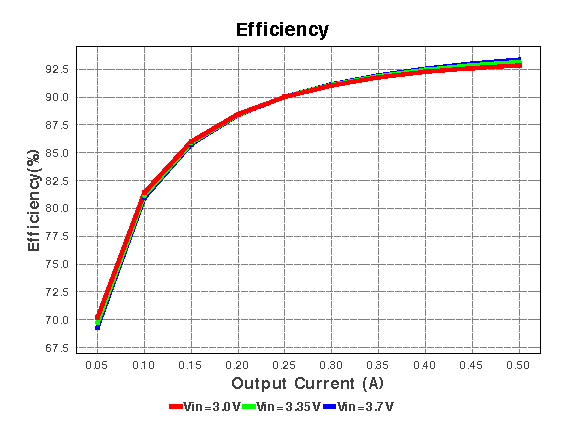
\includegraphics[width=0.8\textwidth]{./images/Efficiency_TPS61088}
	\caption{Efficiency w.r.t. output current}
	\end{center}
\end{figure}

\section{Power Driver}\label{Appendix: powerDriver}
% \begin{figure}[H]
% 	\begin{center}
% 		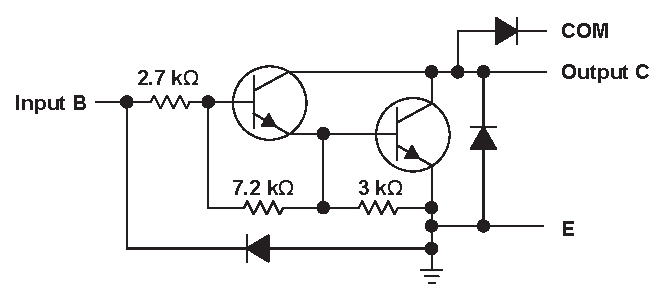
\includegraphics[width=0.8\textwidth]{./images/ULN2803A}
% 	\caption{Functional block diagram of the ULN2803A}
% 	\end{center}
% \end{figure}

\begin{figure}[H]
\centering
\begin{subfigmatrix}{2} 
\hspace*{\fill}%
\subfigure[Functional block diagram] 
	{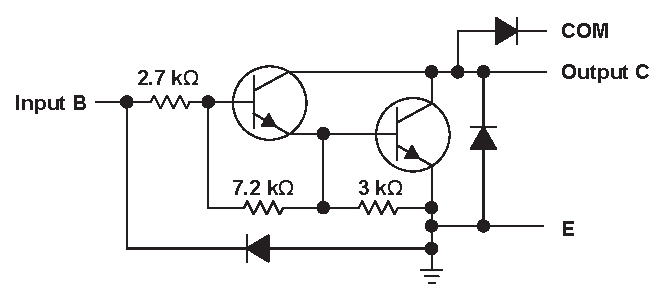
\includegraphics[width=3.0in]{./images/ULN2803A}}\hfill
\subfigure[Top view]
	{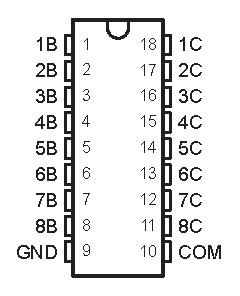
\includegraphics[width=1.0in]{./images/ulnpins}}
\hspace*{\fill}%
\end{subfigmatrix}
\caption{ULN2803 Darlington driver}
\end{figure}


\section{Transmitter}

\begin{figure}[H]
\begin{center}
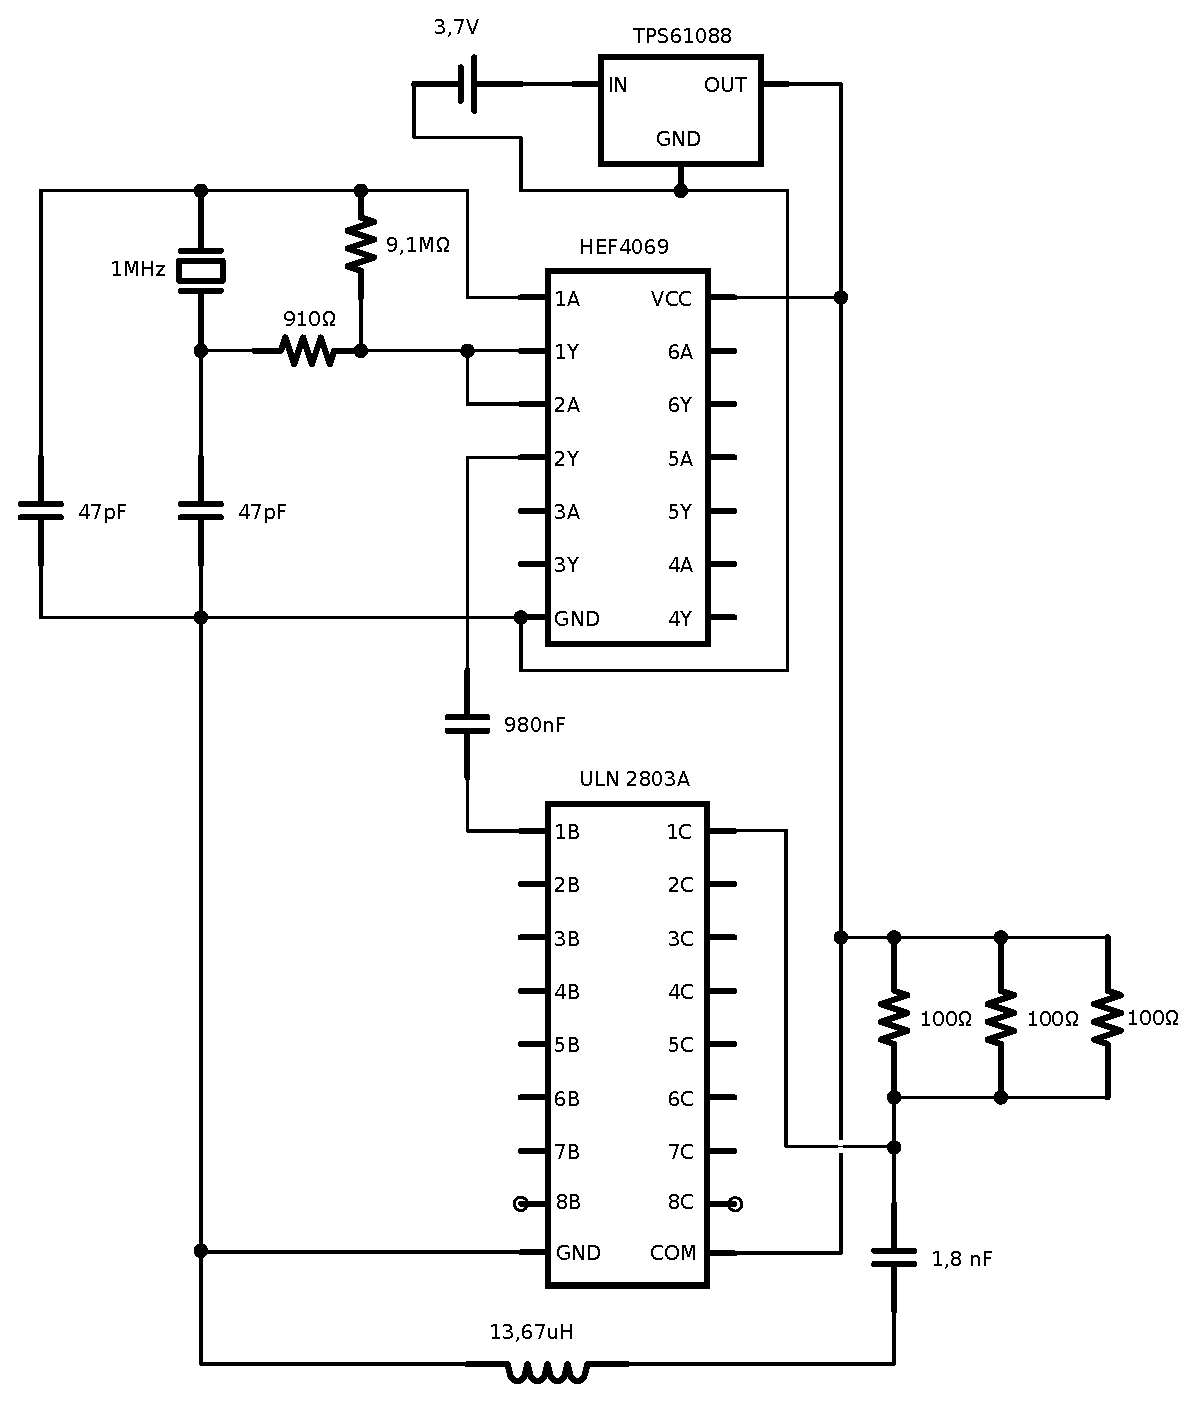
\includegraphics[width=1\textwidth]{./images/circuitv5}
\caption{Transmitter circuit schematic}
% \label{F:contourLines}
\end{center}
\end{figure}

\section{Receiver}
\begin{figure}[H]
\begin{center}
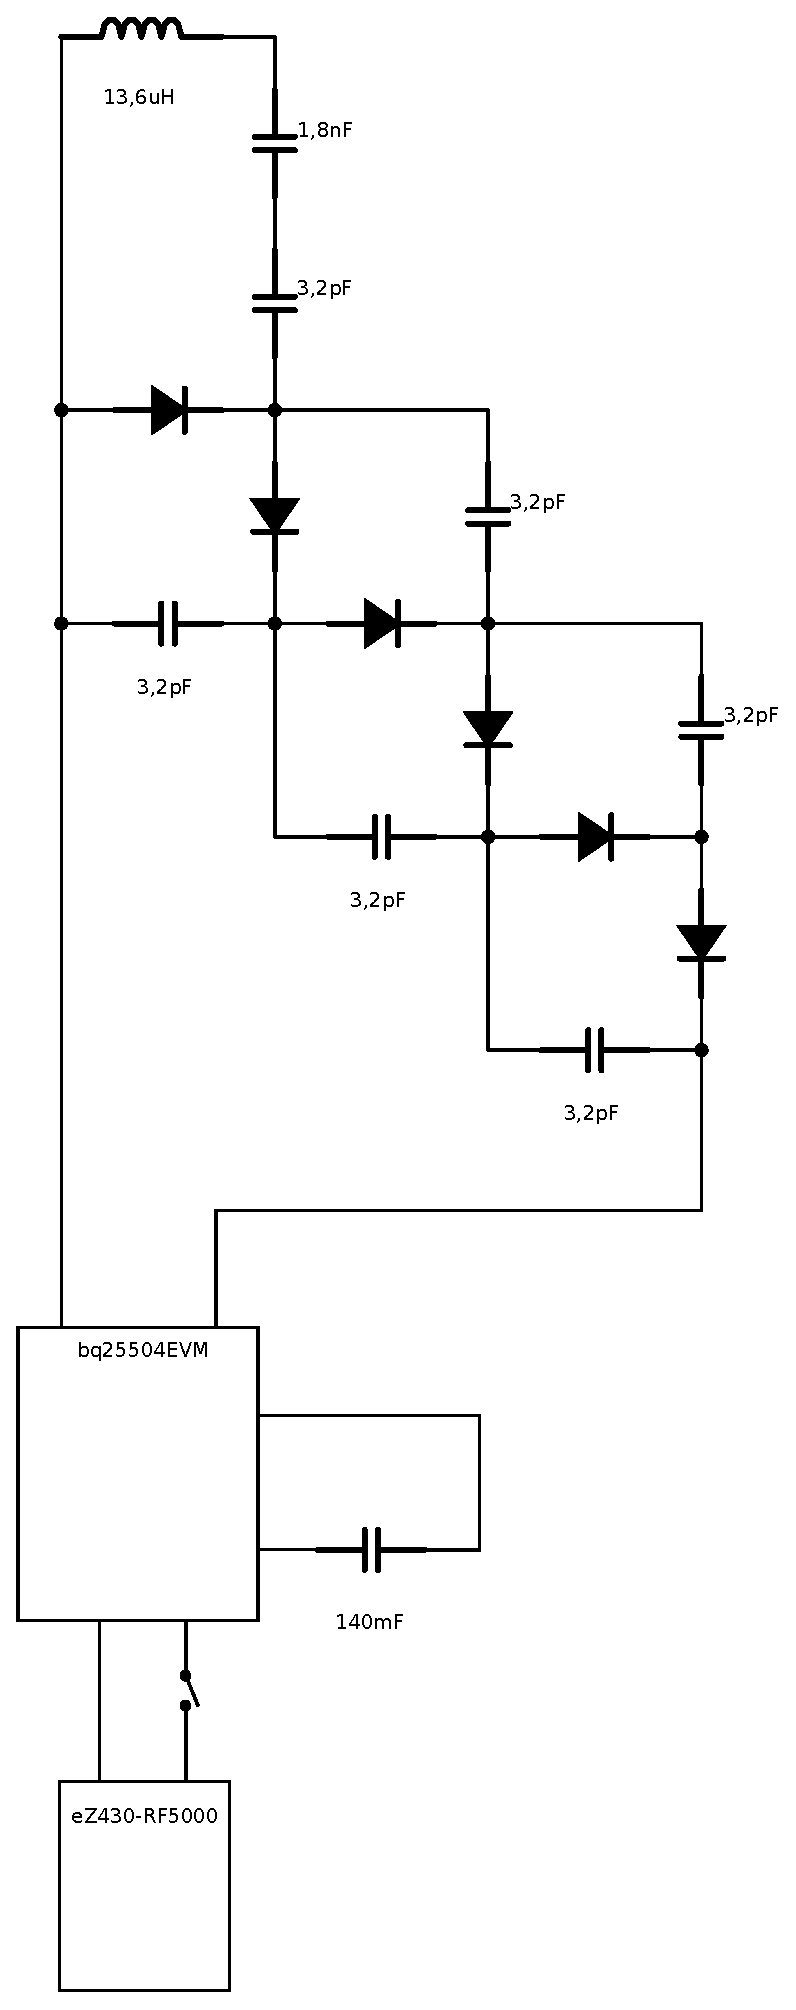
\includegraphics[width=0.55\textwidth]{./images/ReceiverSchematic}
\caption{Receiver circuit schematic}
% \label{F:contourLines}
\end{center}
\end{figure}









\chapter{Experimental Results} \label{Appendix: experimental}

\section{Model A}

\begin{figure}[h]
\centering
\begin{subfigmatrix}{2} 
\subfigure[f = 0.7 MHz]
{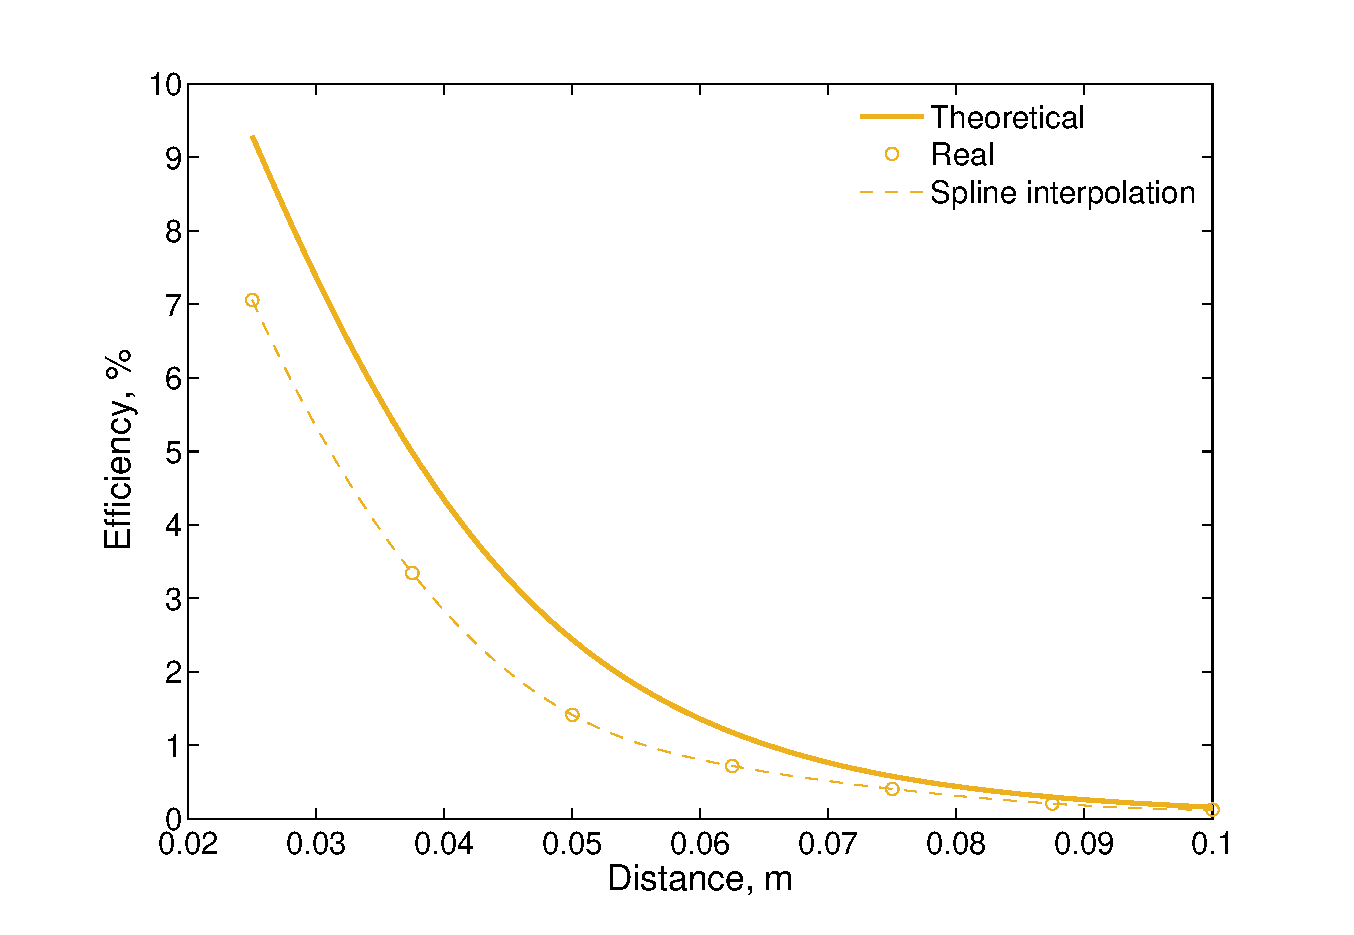
\includegraphics{./images/ModeloS_A_2_eff}}
\subfigure[f = 1 MHz]
{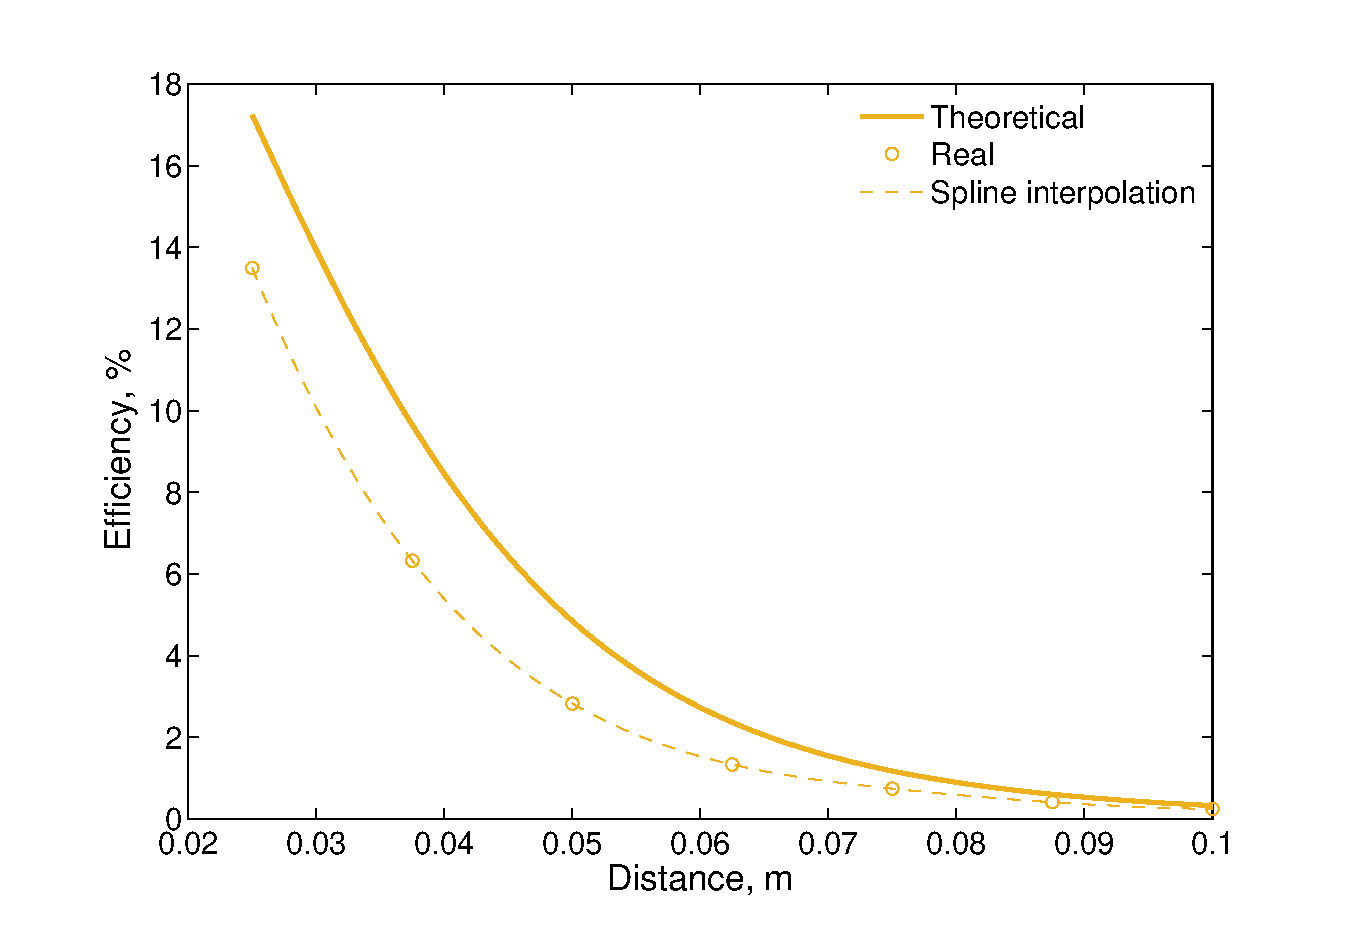
\includegraphics{./images/ModeloS_A_1_eff}}
\end{subfigmatrix}
\end{figure}
% \\[1pt]
\begin{figure}[H]
\centering
\begin{subfigmatrix}{1} 
\subfigure[f = 2 MHz] 
{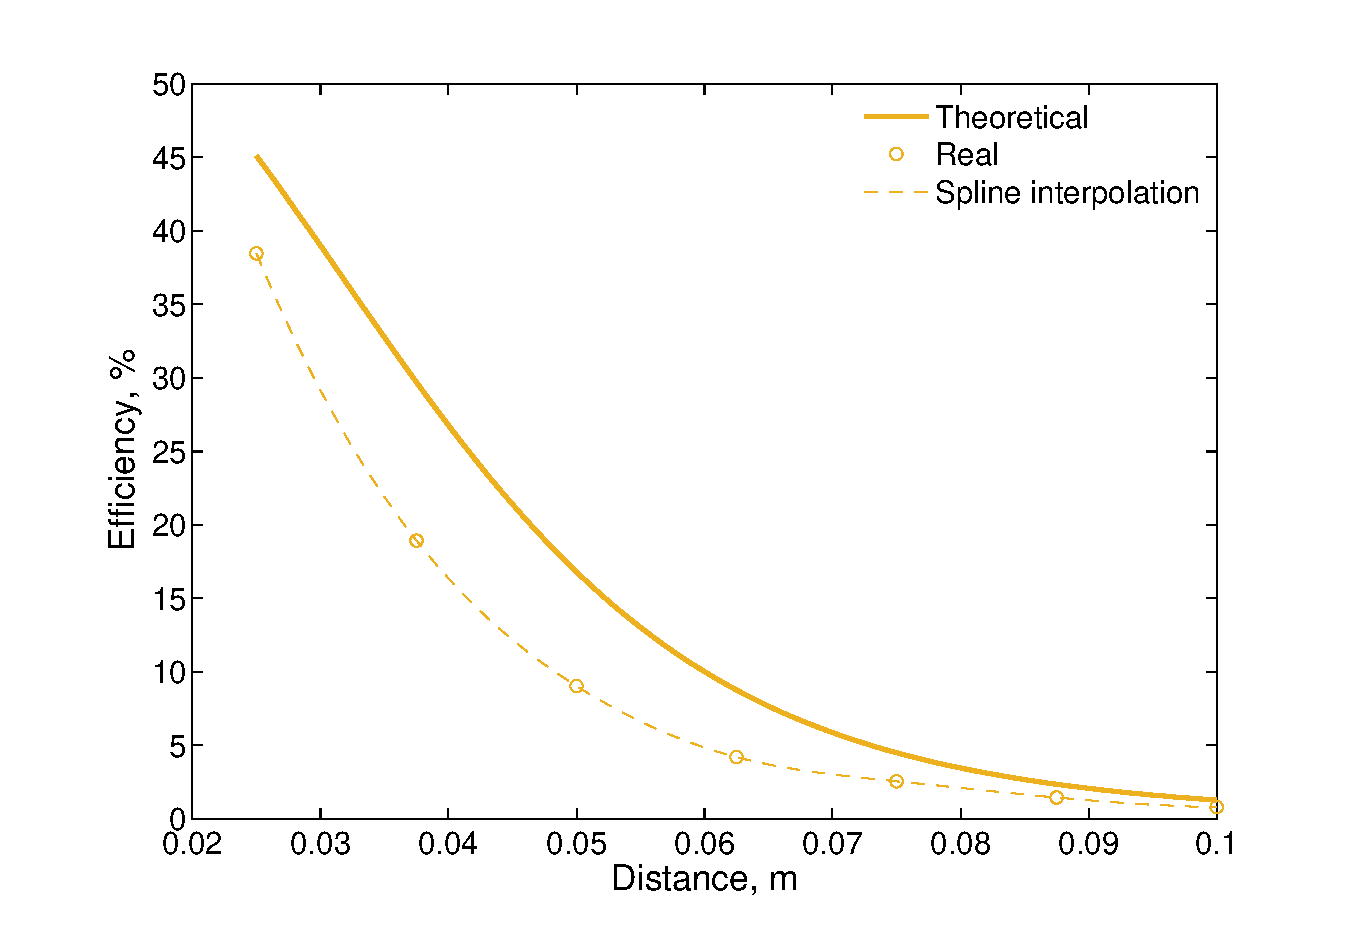
\includegraphics[width=0.5\textwidth]{./images/ModeloS_A_3_eff}}
\end{subfigmatrix}
\caption{Efficiency w.r.t. distance for SS topology}
\end{figure}

%%%%%%%%%%%%%%%%%%%%%%%%%%%%%%%%%%%%%%%%%%%%%%%%

\begin{figure}[h]
\centering
\begin{subfigmatrix}{2} 
\subfigure[f = 0.7 MHz]
{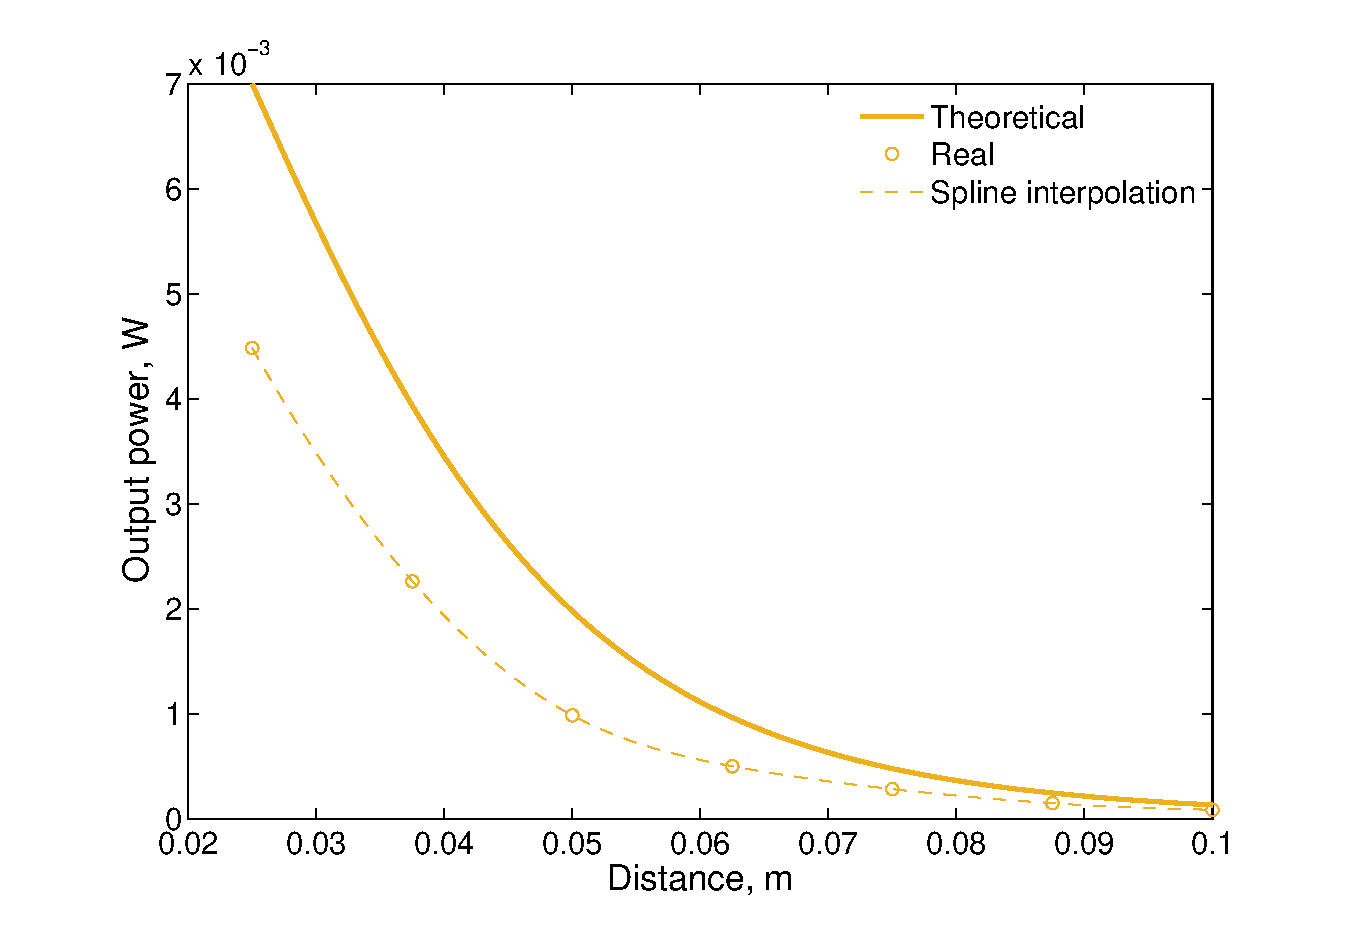
\includegraphics{./images/ModeloS_A_2_pout}}
\subfigure[f = 1 MHz]
{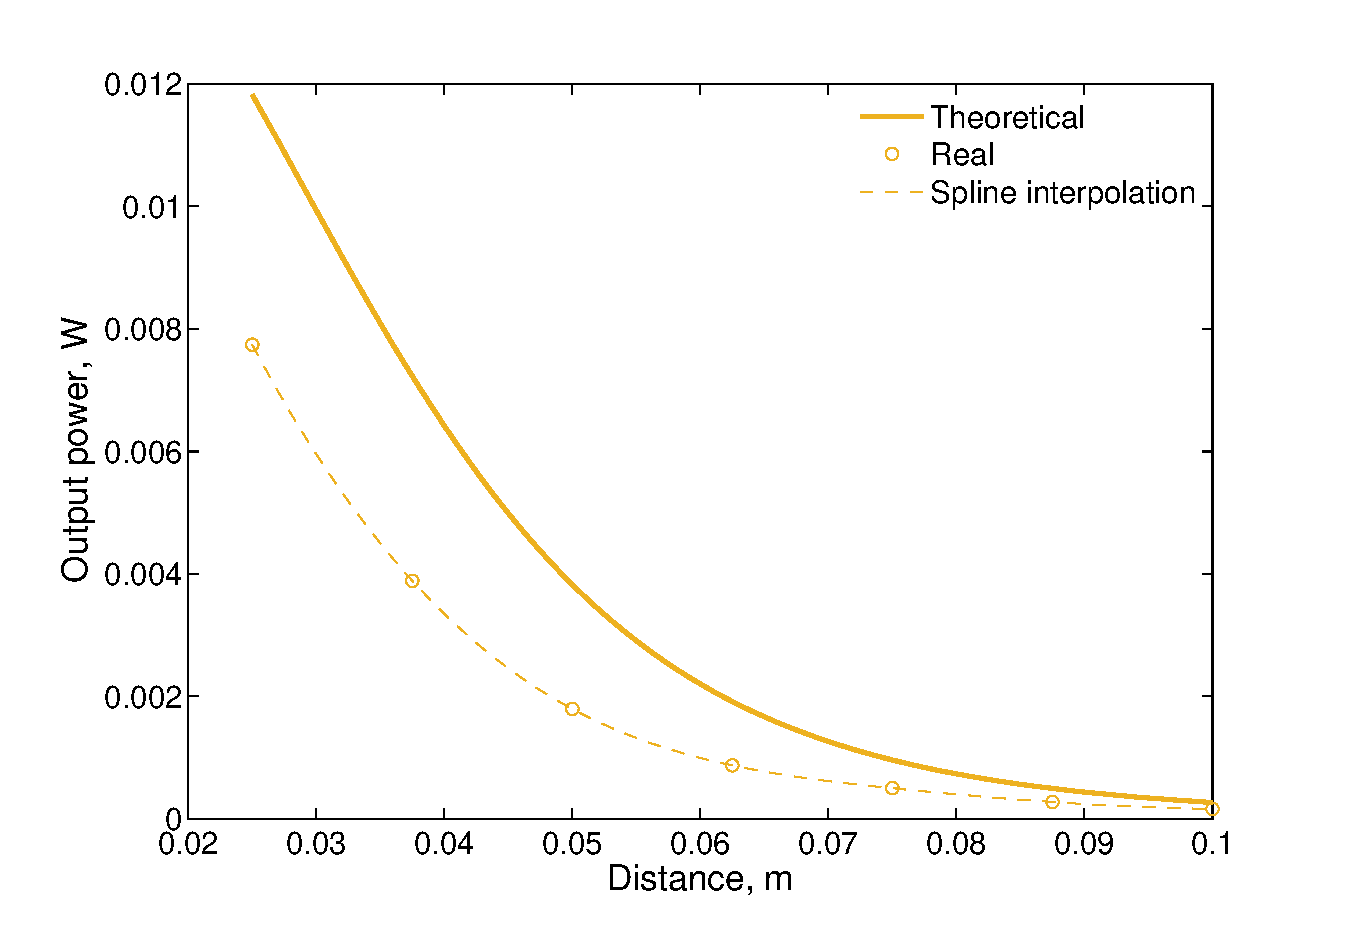
\includegraphics{./images/ModeloS_A_1_pout}}
\end{subfigmatrix}
\end{figure}
\begin{figure}[H]
\centering
\begin{subfigmatrix}{1} 
\subfigure[f = 2 MHz] 
{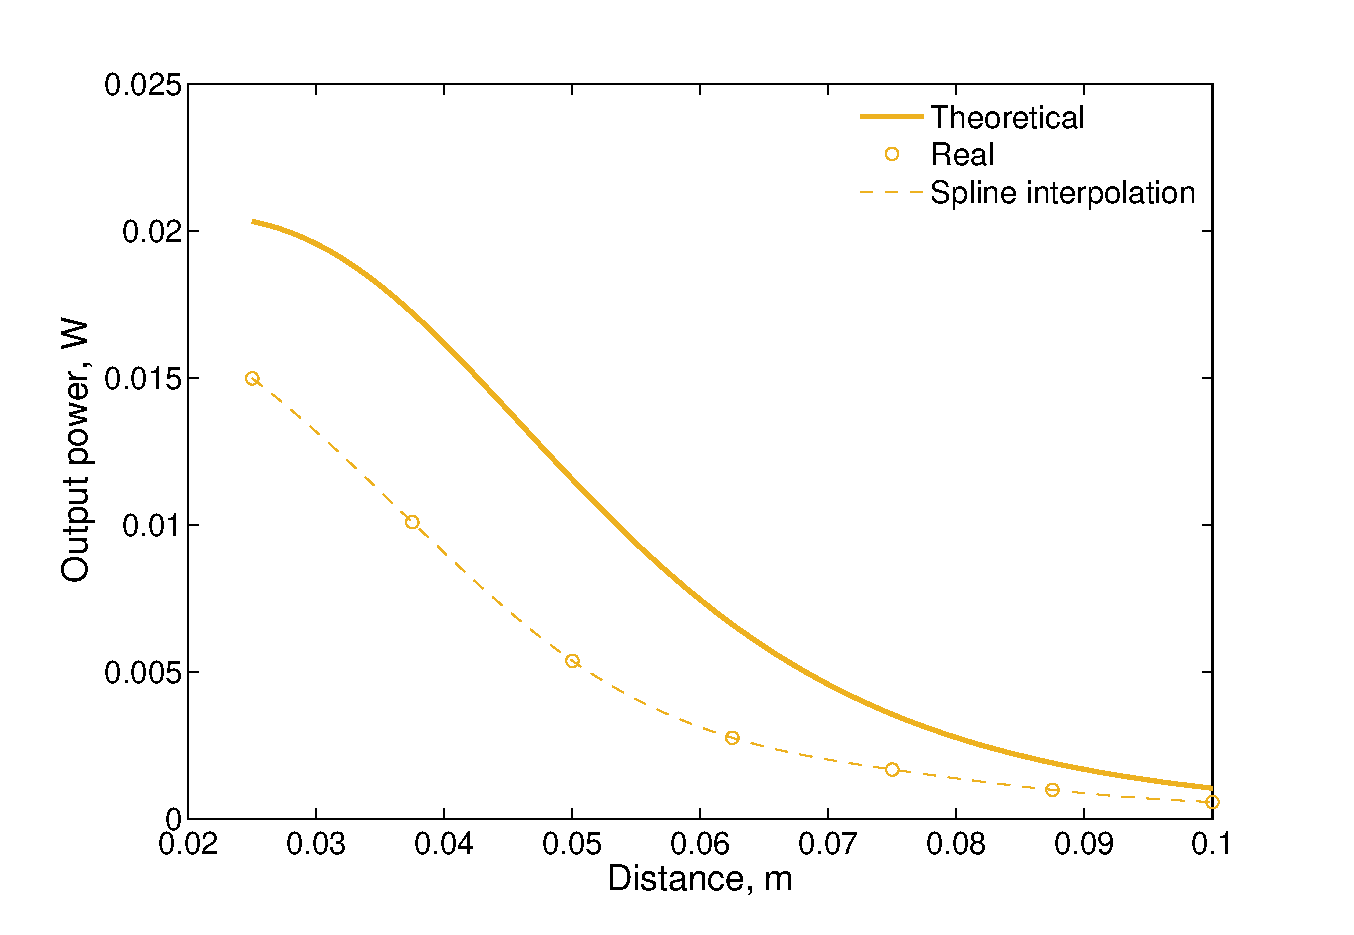
\includegraphics[width=0.5\textwidth]{./images/ModeloS_A_3_pout}}
\end{subfigmatrix}
\caption{Output power w.r.t. distance for SS topology}
\end{figure}

%%%%%%%%%%%%%%%%%%%%%%%%%%%%%%%%%%%%%%%%%%%%%%%%

\begin{figure}[h]
\centering
\begin{subfigmatrix}{2} 
\subfigure[f = 0.7 MHz]
{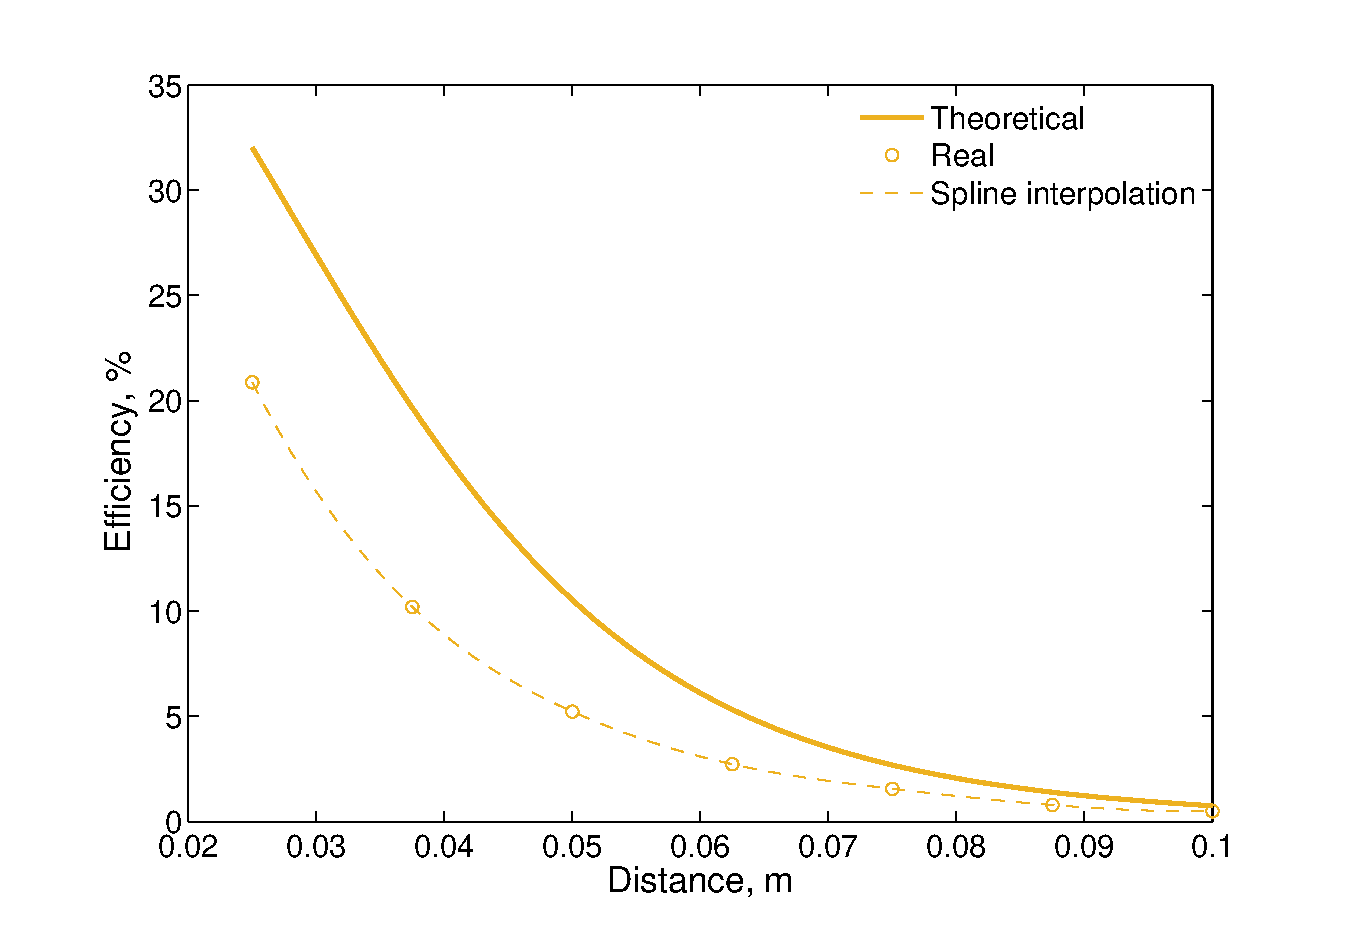
\includegraphics{./images/ModeloP_A_2_eff}}
\subfigure[f = 1 MHz]
{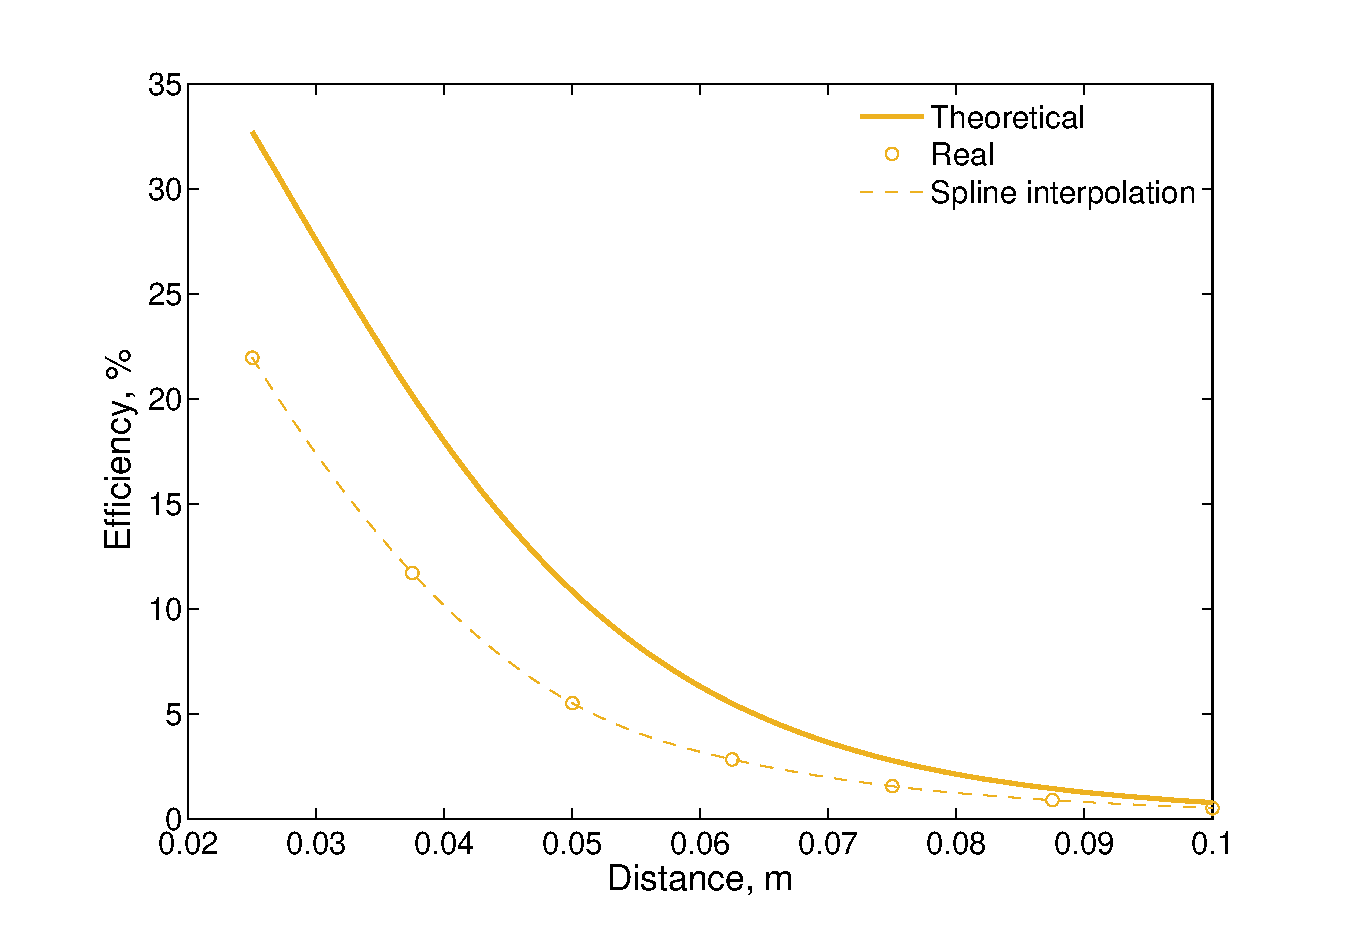
\includegraphics{./images/ModeloP_A_1_eff}}
\end{subfigmatrix}
\end{figure}
\begin{figure}[H]
\centering
\begin{subfigmatrix}{1} 
\subfigure[f = 2 MHz] 
{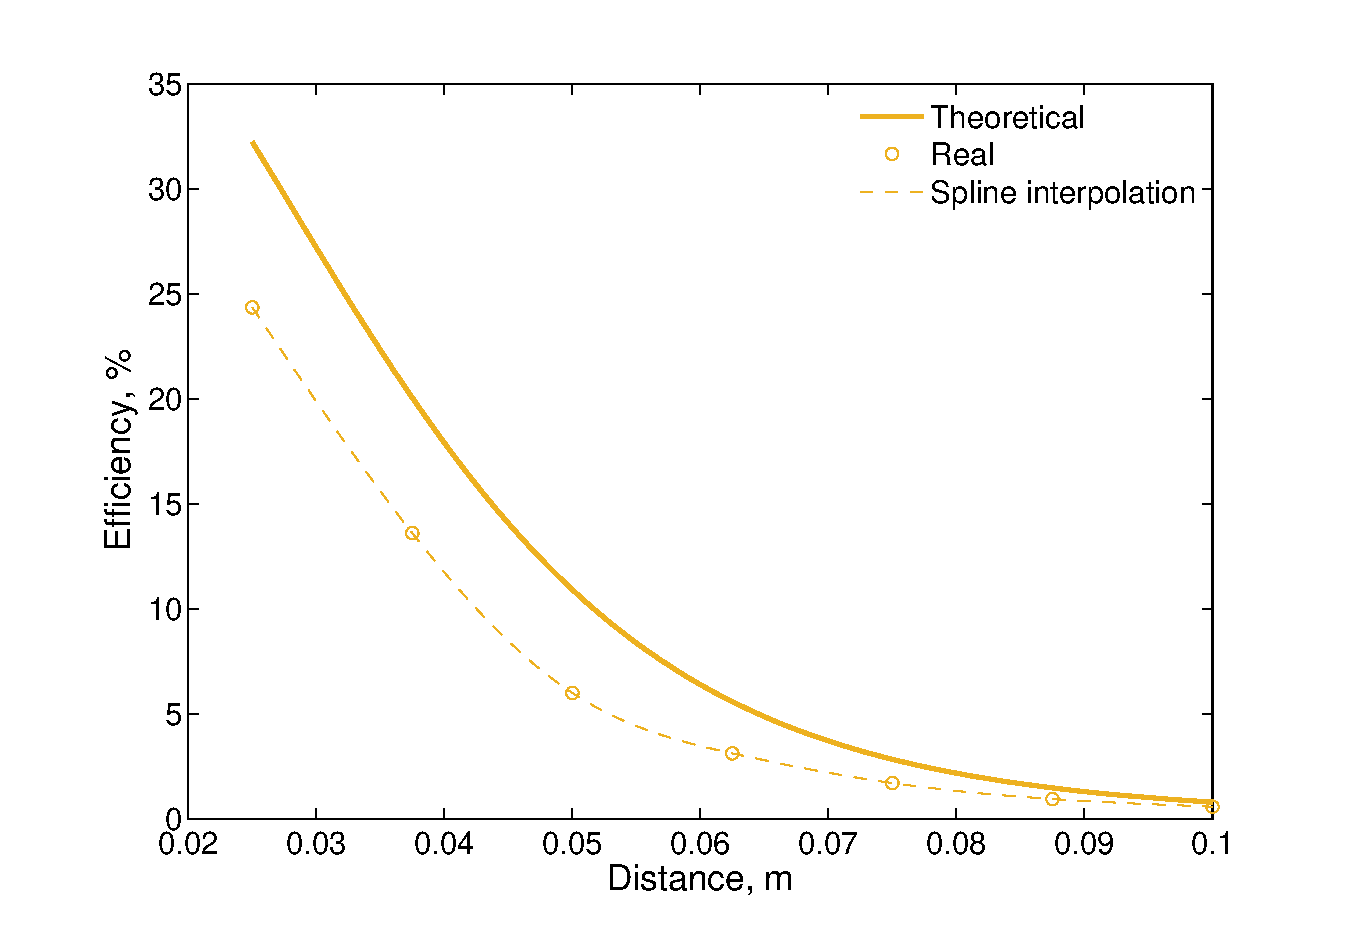
\includegraphics[width=0.5\textwidth]{./images/ModeloP_A_3_eff}}
\end{subfigmatrix}
\caption{Efficiency w.r.t. distance for SP topology}
\end{figure}

%%%%%%%%%%%%%%%%%%%%%%%%%%%%%%%%%%%%%%%%%%%%%%%%

\begin{figure}[h]
\centering
\begin{subfigmatrix}{2} 
\subfigure[f = 0.7 MHz]
{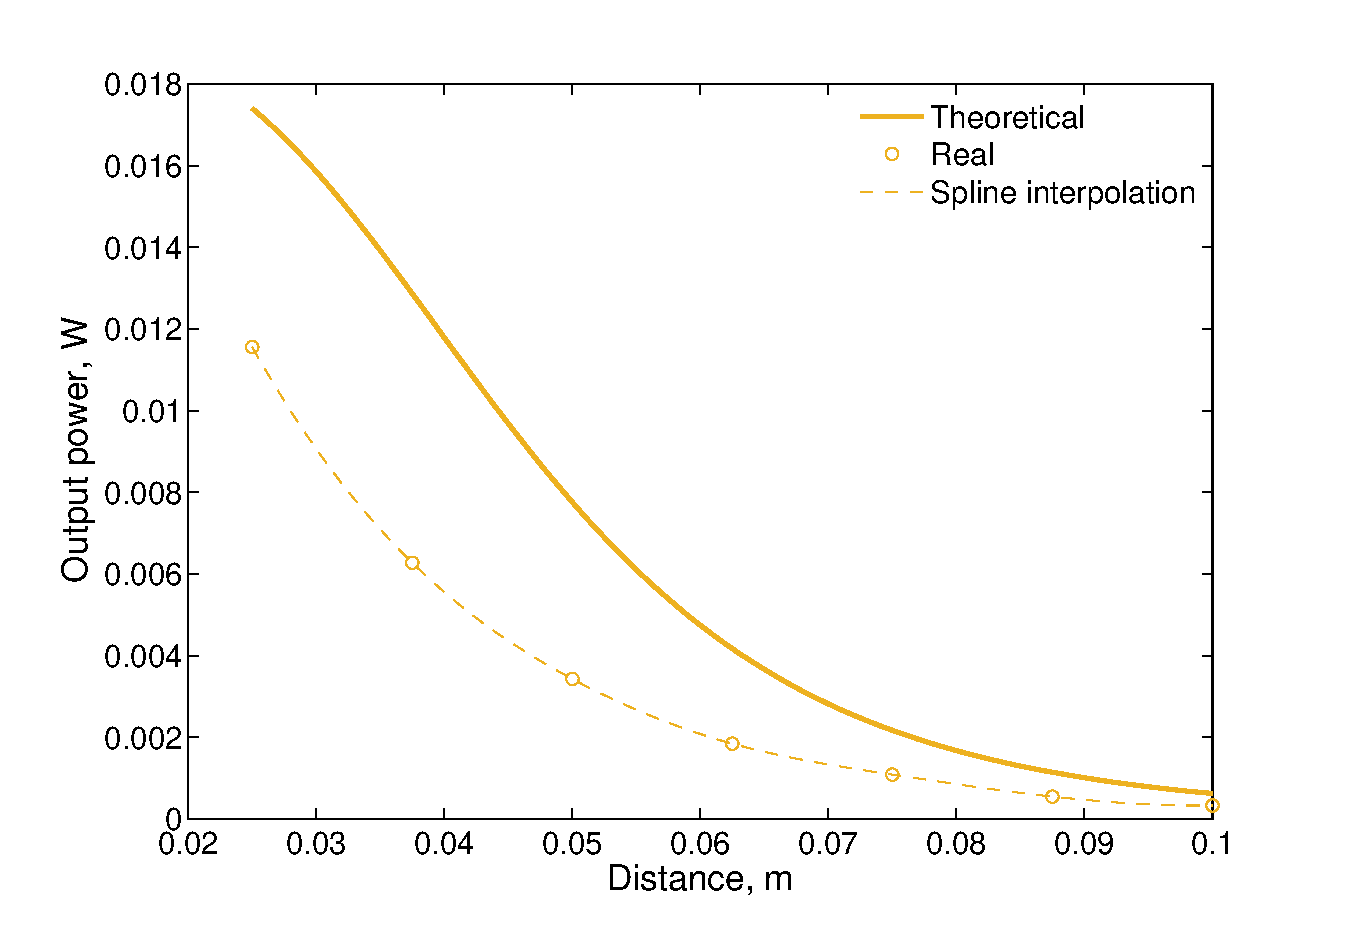
\includegraphics{./images/ModeloP_A_2_pout}}
\subfigure[f = 1 MHz]
{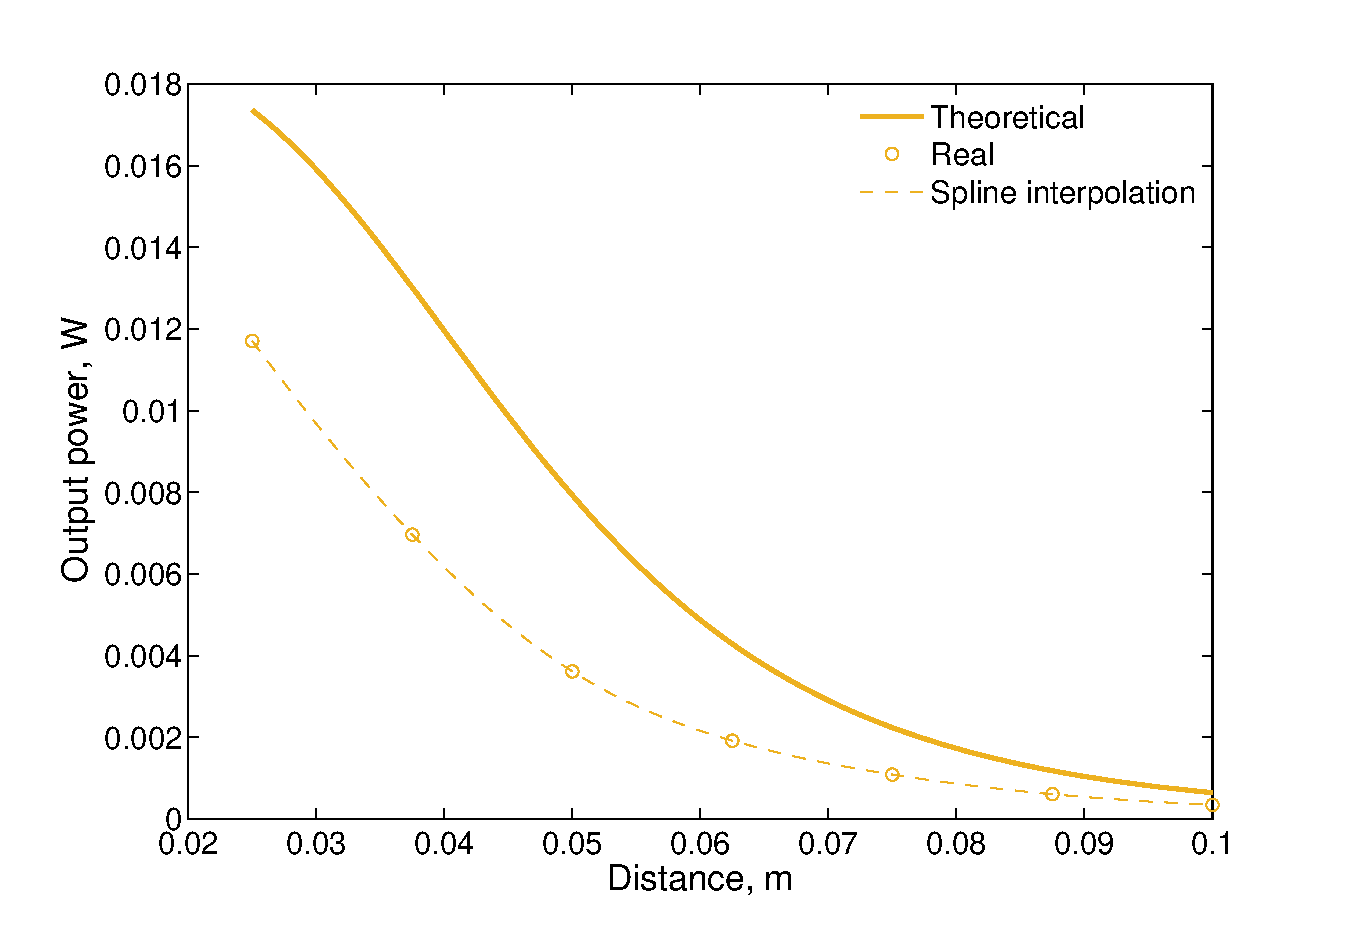
\includegraphics{./images/ModeloP_A_1_pout}}
\end{subfigmatrix}
\end{figure}
\begin{figure}[H]
\centering
\begin{subfigmatrix}{1} 
\subfigure[f = 2 MHz] 
{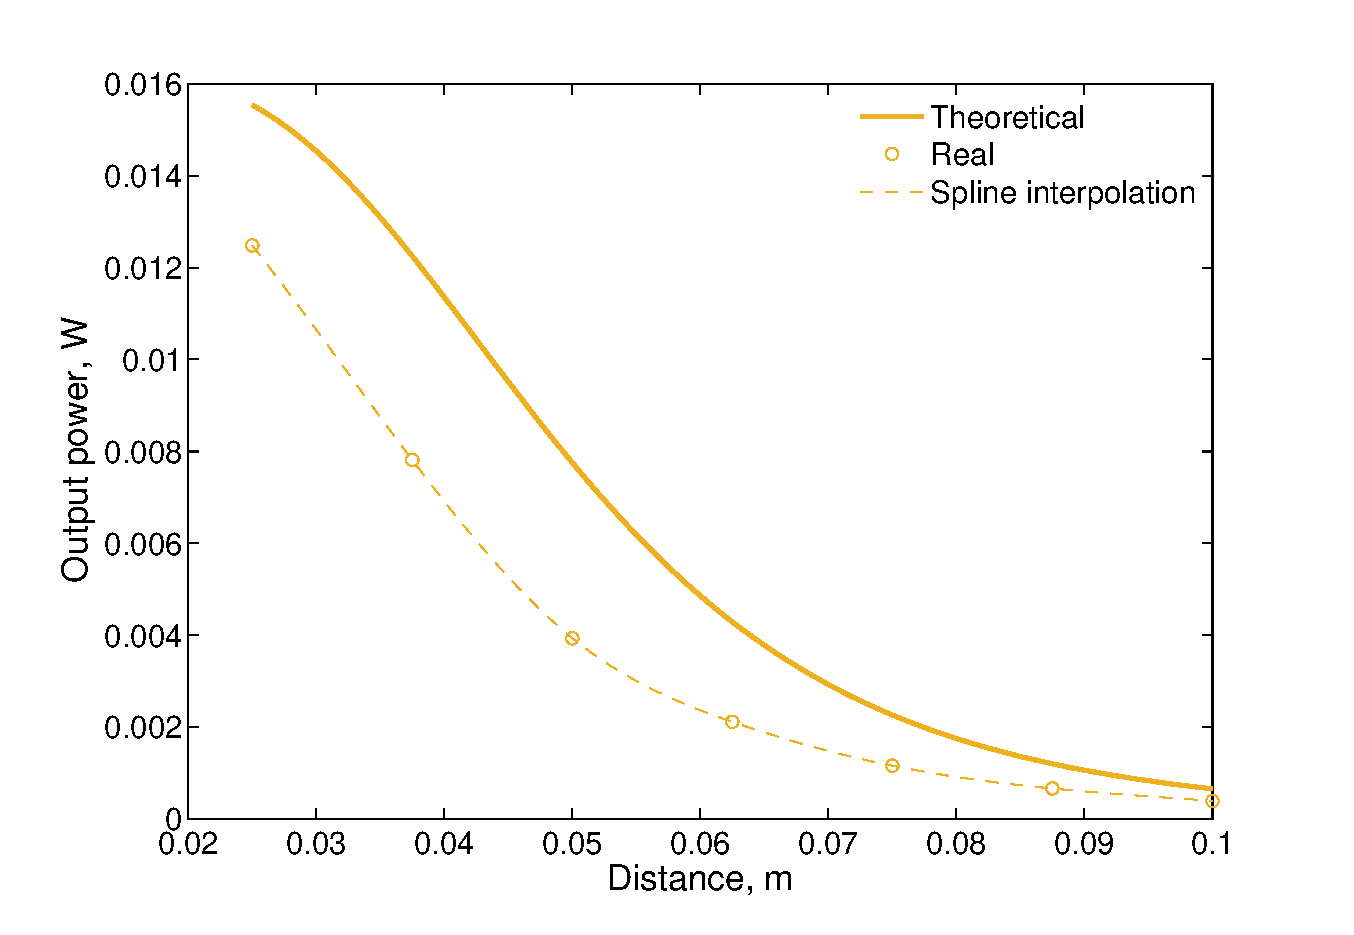
\includegraphics[width=0.5\textwidth]{./images/ModeloP_A_3_pout}}
\end{subfigmatrix}
\caption{Output power w.r.t. distance for SP topology}
\end{figure}

%%%%%%%%%%%%%%%%%%%%%%%%%%%%%%%%%%%%%%%%%%%%%%%%

\begin{figure}[h]
\centering
\begin{subfigmatrix}{2} 
\subfigure[f = 0.7 MHz]
{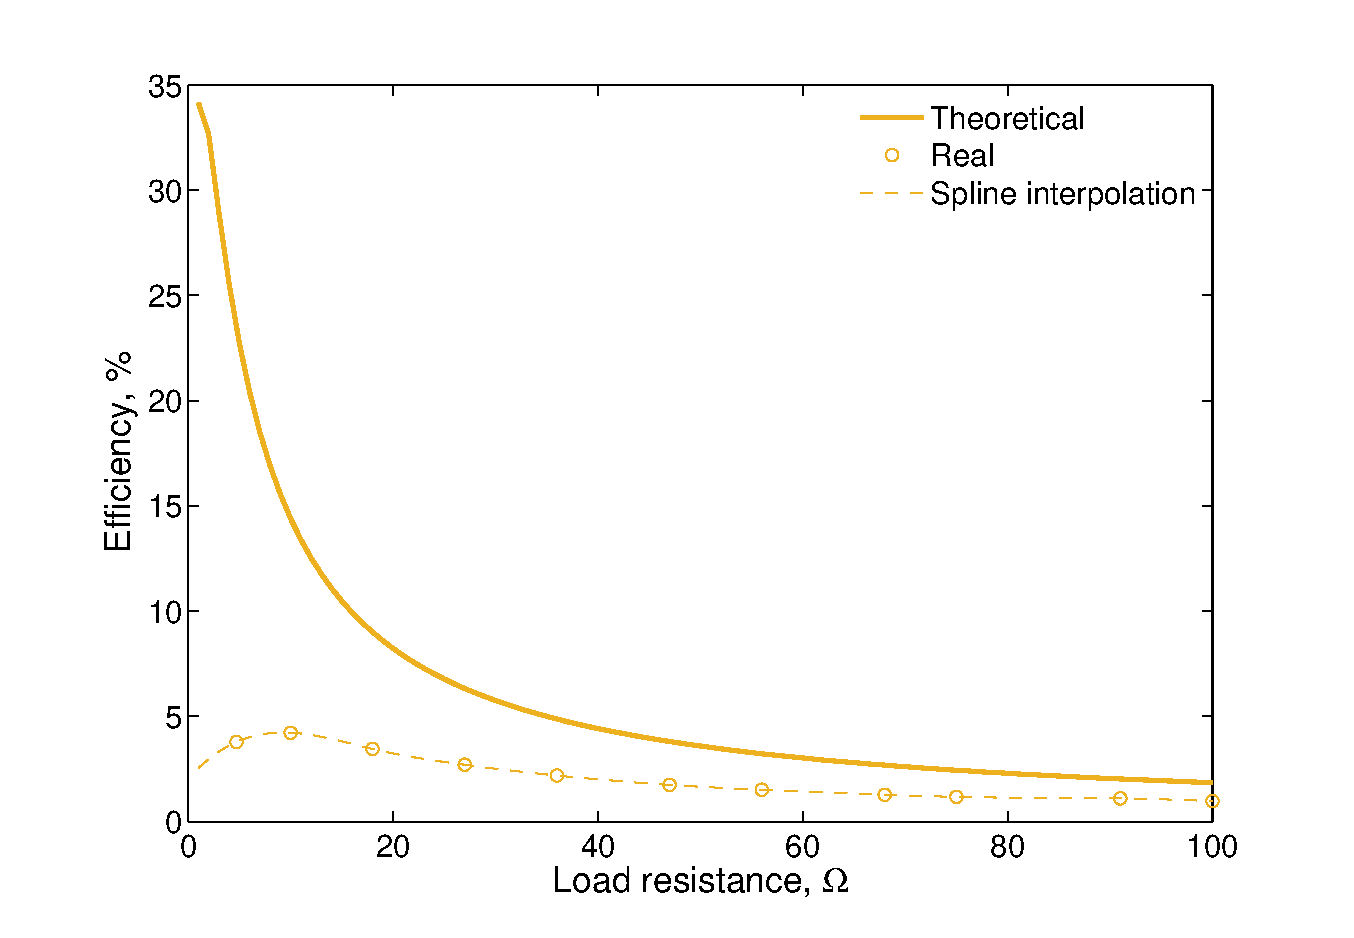
\includegraphics{./images/ModeloS_A_ZL_2_eff}}
\subfigure[f = 1 MHz]
{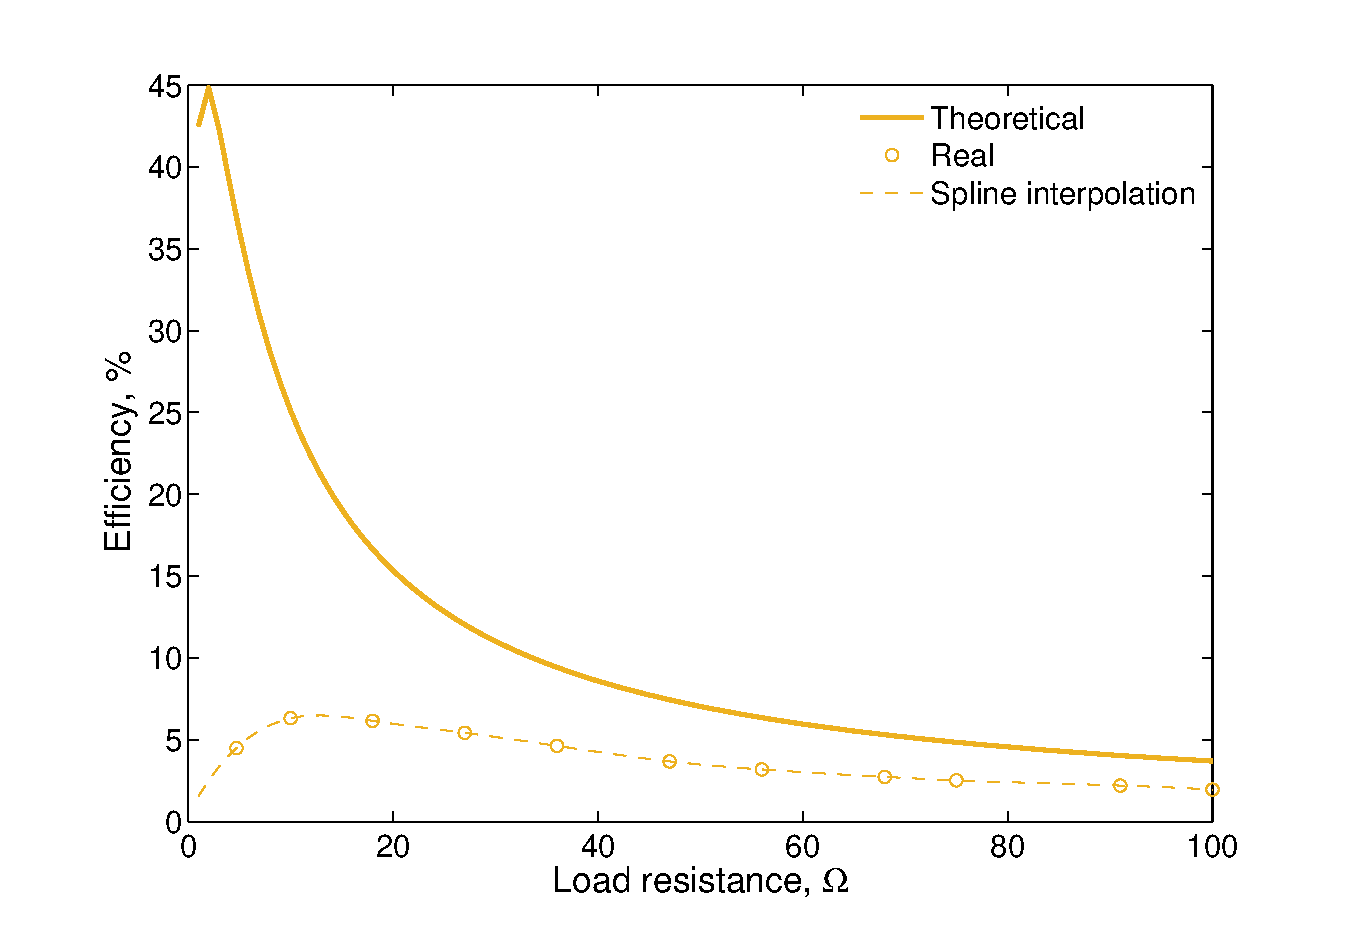
\includegraphics{./images/ModeloS_A_ZL_1_eff}}
\end{subfigmatrix}
\end{figure}
\begin{figure}[H]
\centering
\begin{subfigmatrix}{1} 
\subfigure[f = 2 MHz] 
{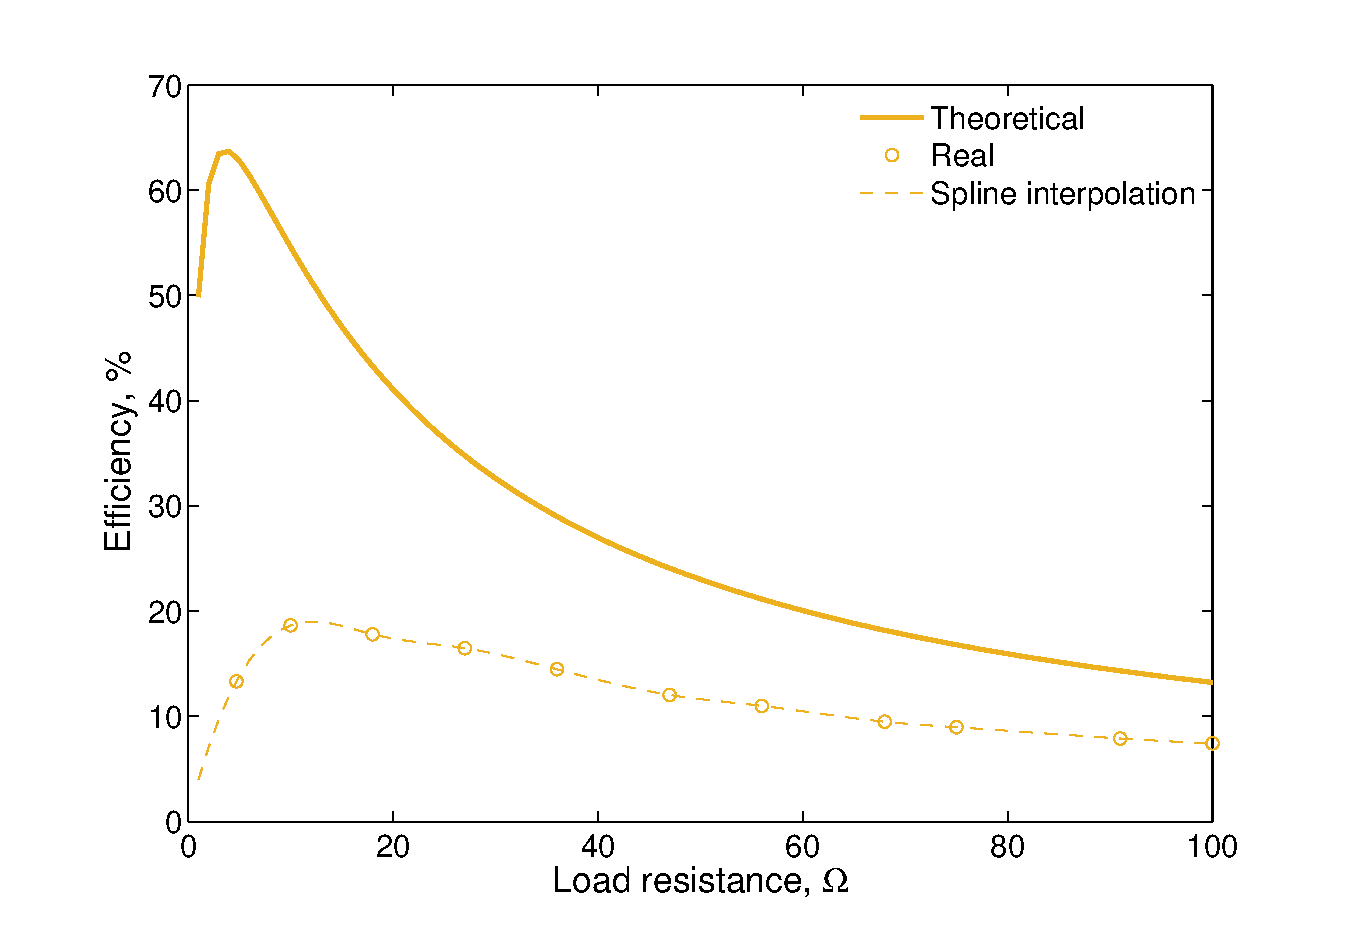
\includegraphics[width=0.5\textwidth]{./images/ModeloS_A_ZL_3_eff}}
\end{subfigmatrix}
\caption{Efficiency w.r.t. load resistance for SS topology}
\end{figure}

%%%%%%%%%%%%%%%%%%%%%%%%%%%%%%%%%%%%%%%%%%%%%%%%

\begin{figure}[h]
\centering
\begin{subfigmatrix}{2} 
\subfigure[f = 0.7 MHz]
{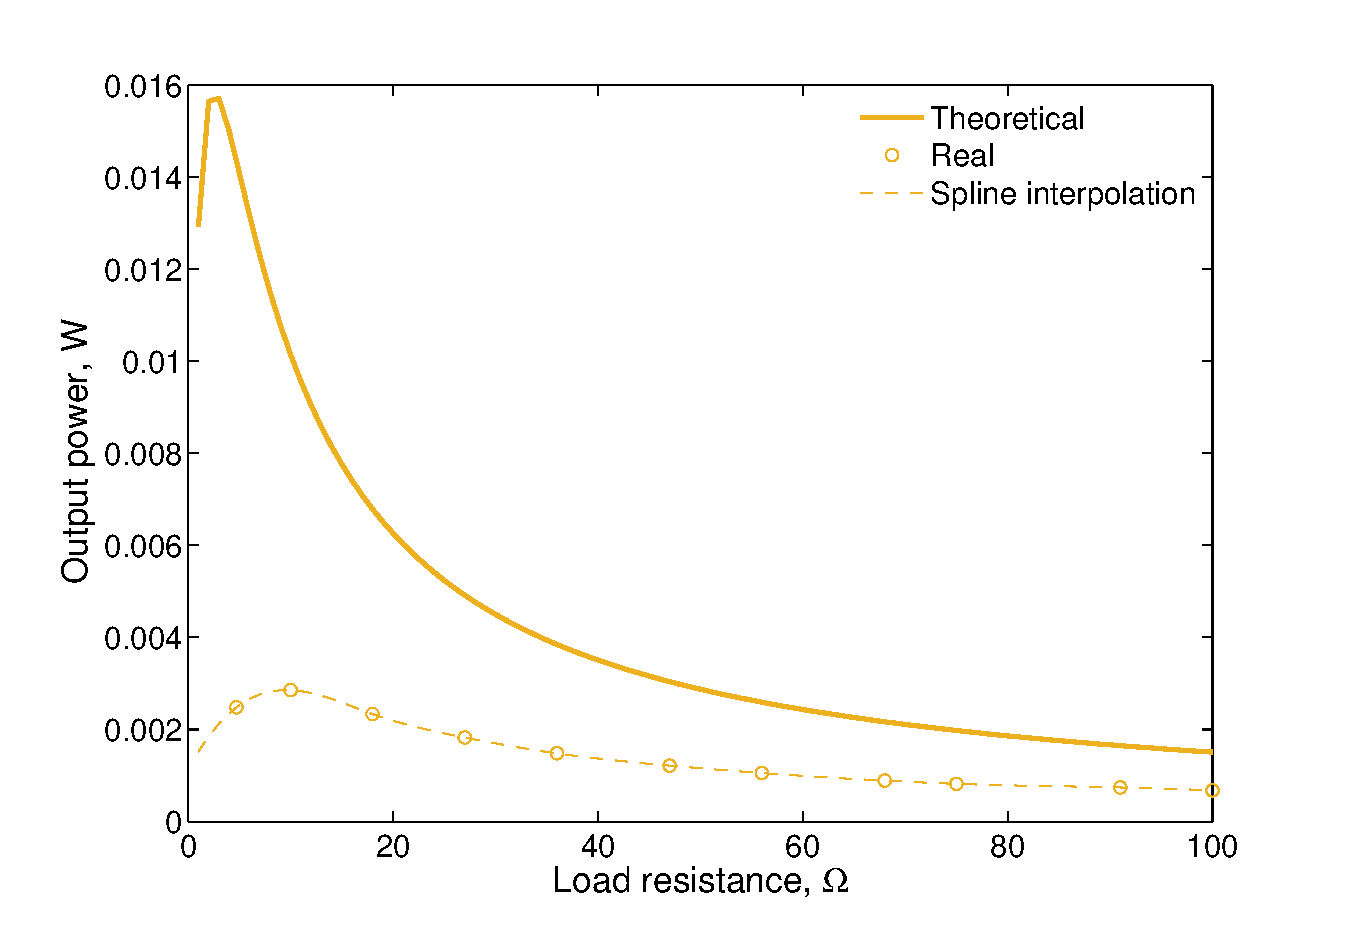
\includegraphics{./images/ModeloS_A_ZL_2_pout}}
\subfigure[f = 1 MHz]
{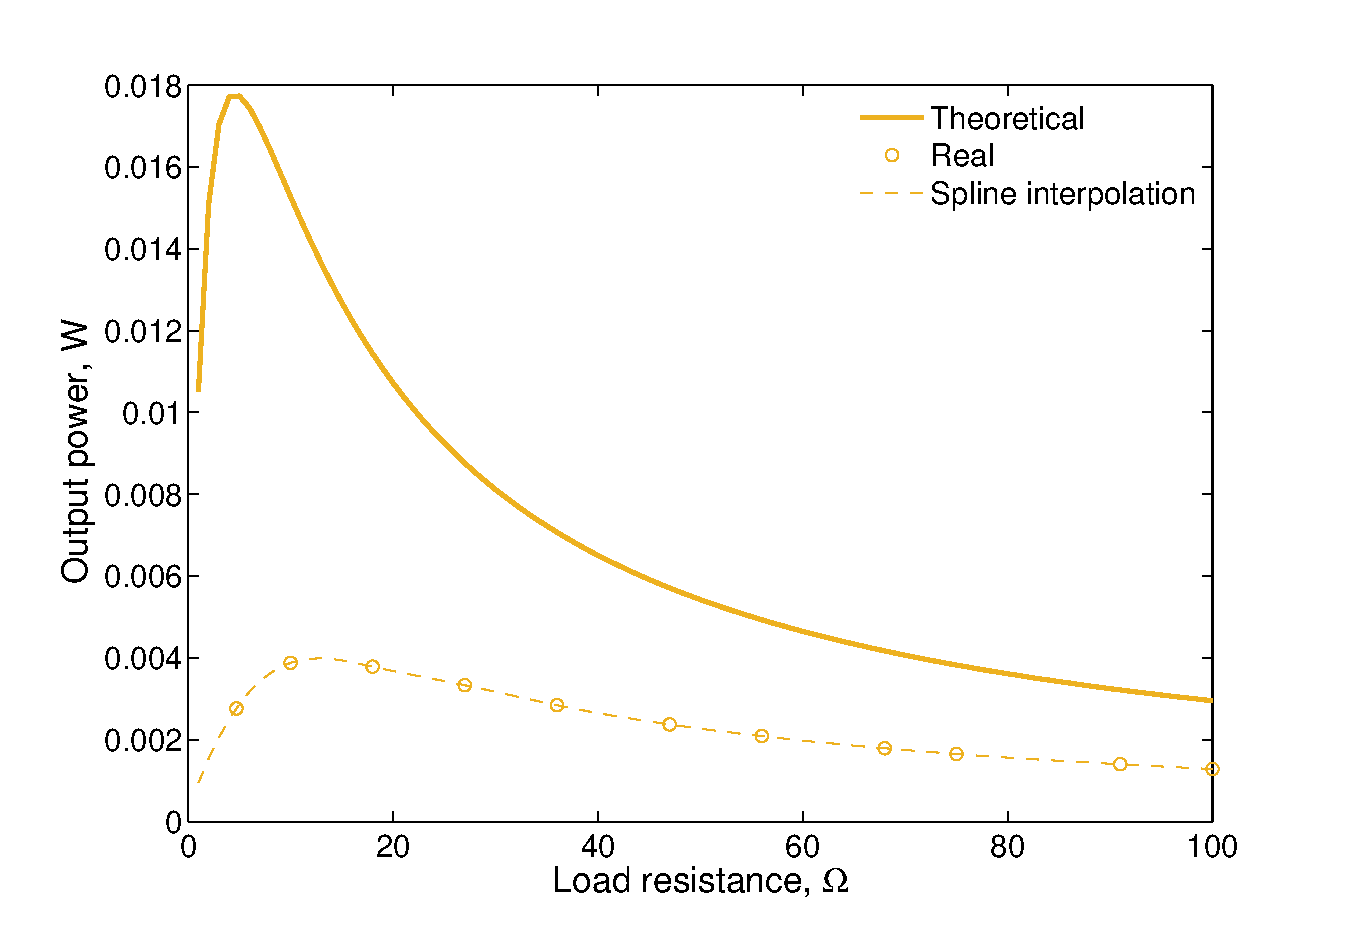
\includegraphics{./images/ModeloS_A_ZL_1_pout}}
\end{subfigmatrix}
\end{figure}
\begin{figure}[H]
\centering
\begin{subfigmatrix}{1} 
\subfigure[f = 2 MHz] 
{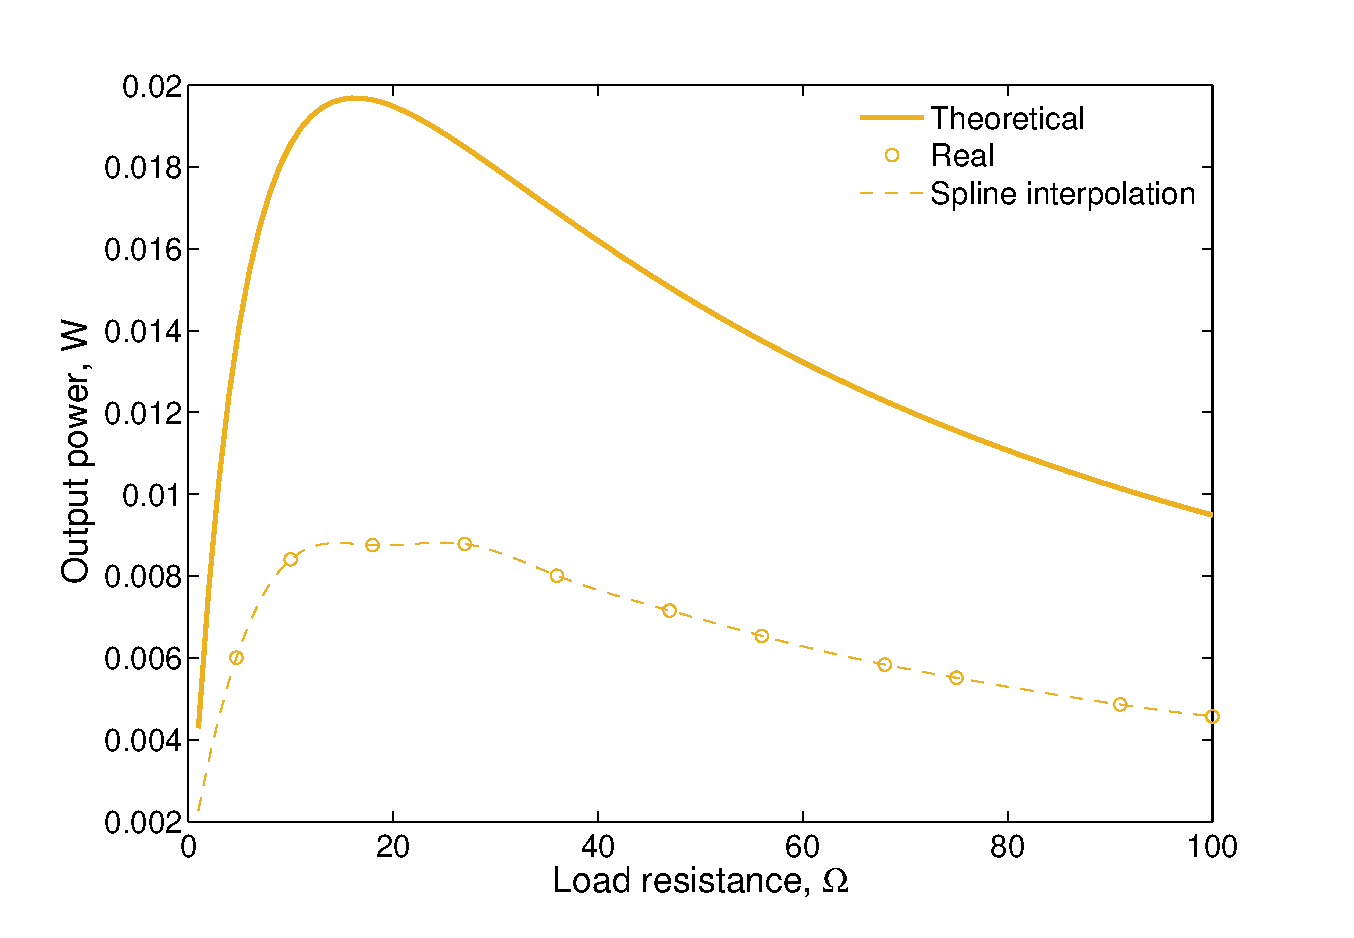
\includegraphics[width=0.5\textwidth]{./images/ModeloS_A_ZL_3_pout}}
\end{subfigmatrix}
\caption{Output power w.r.t. load resistance for SS topology}
\end{figure}

%%%%%%%%%%%%%%%%%%%%%%%%%%%%%%%%%%%%%%%%%%%%%%%%

\begin{figure}[h]
\centering
\begin{subfigmatrix}{2} 
\subfigure[f = 0.7 MHz]
{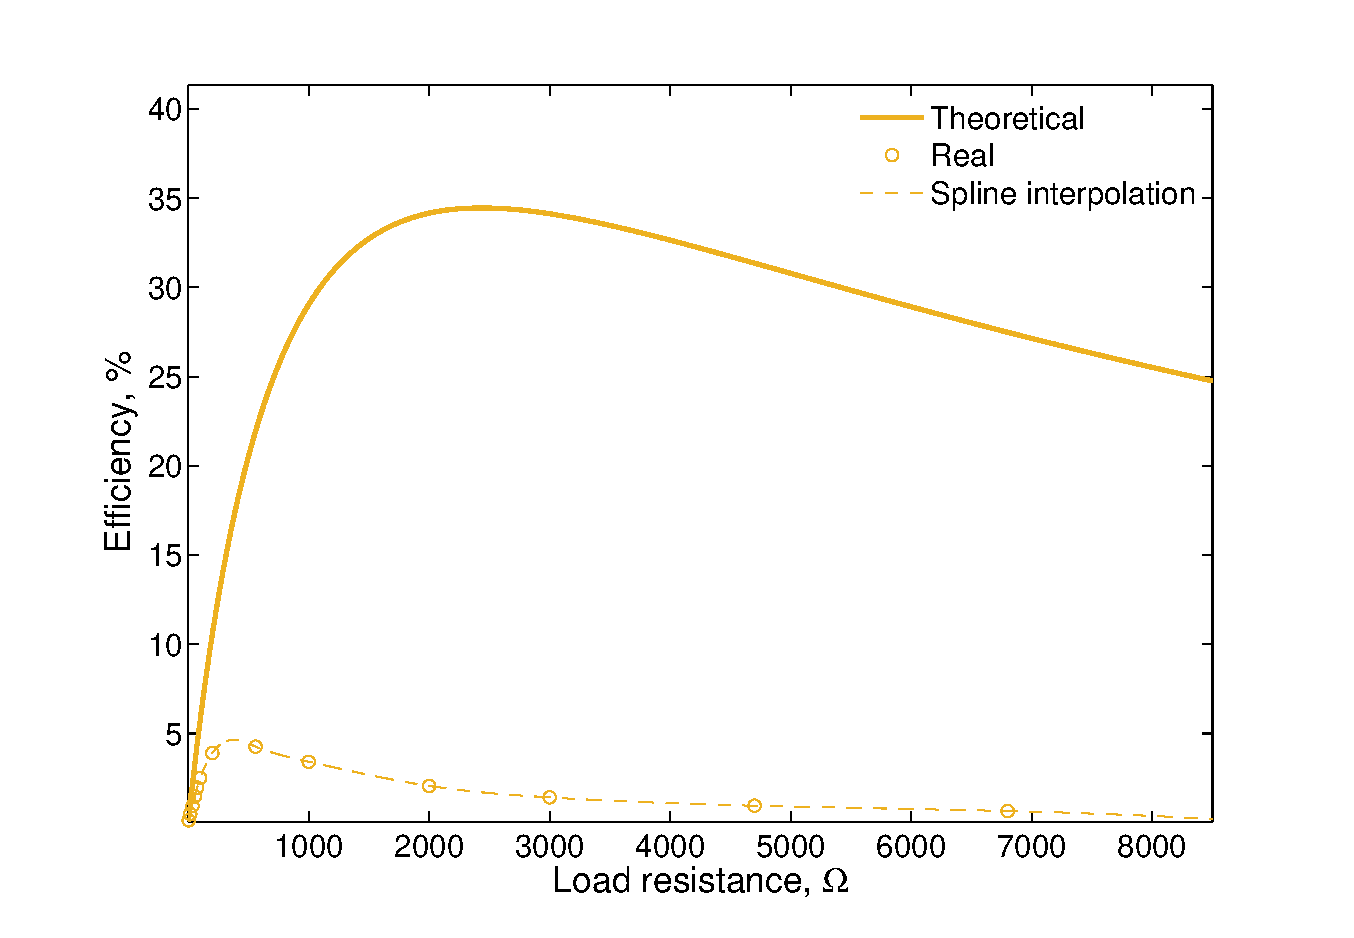
\includegraphics{./images/ModeloP_A_ZL_2_eff}}
\subfigure[f = 1 MHz]
{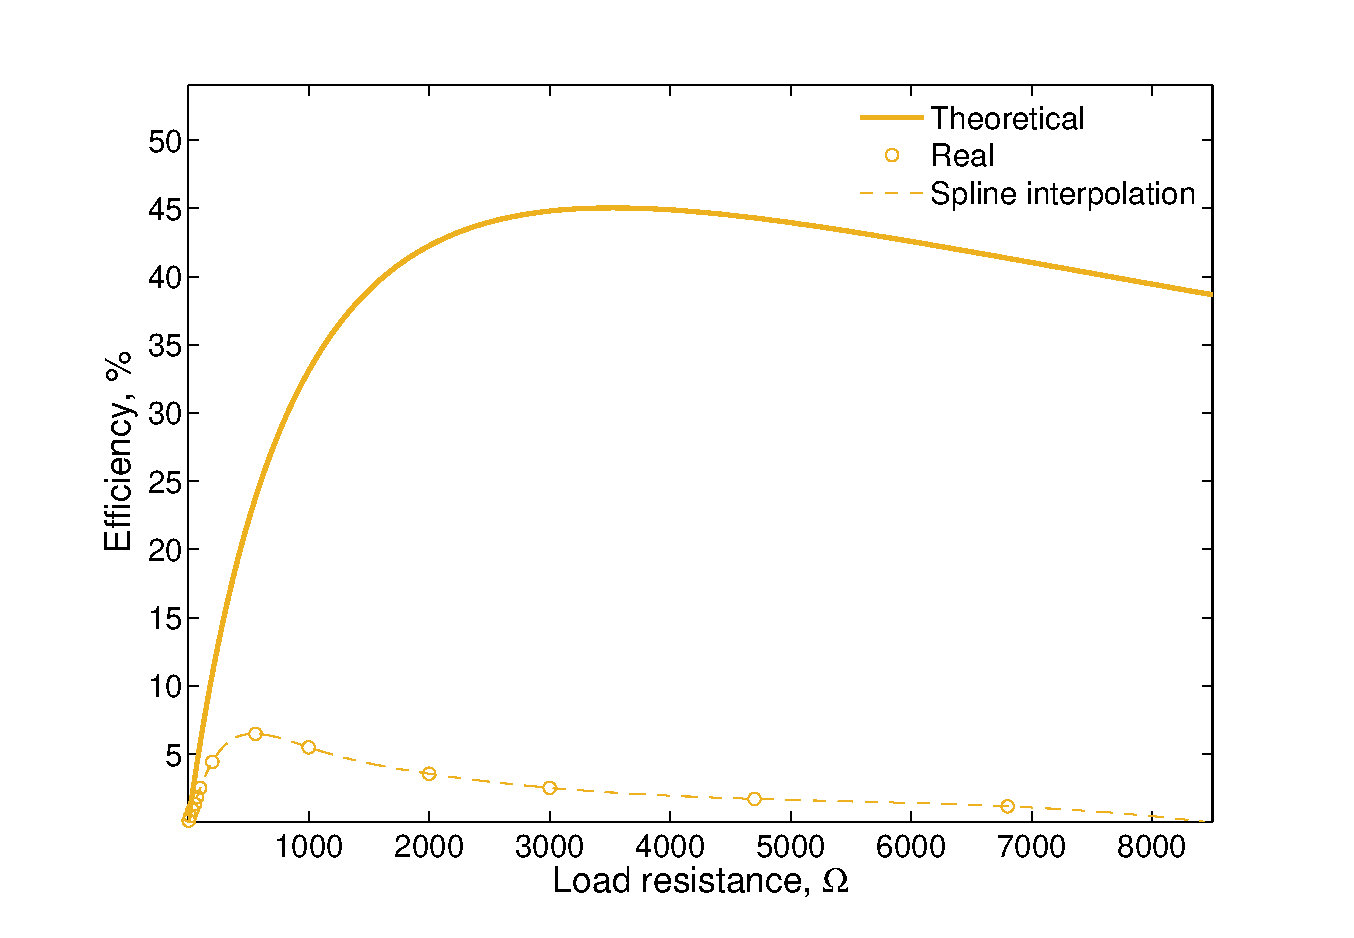
\includegraphics{./images/ModeloP_A_ZL_1_eff}}
\end{subfigmatrix}
\end{figure}
\begin{figure}[H]
\centering
\begin{subfigmatrix}{1} 
\subfigure[f = 2 MHz] 
{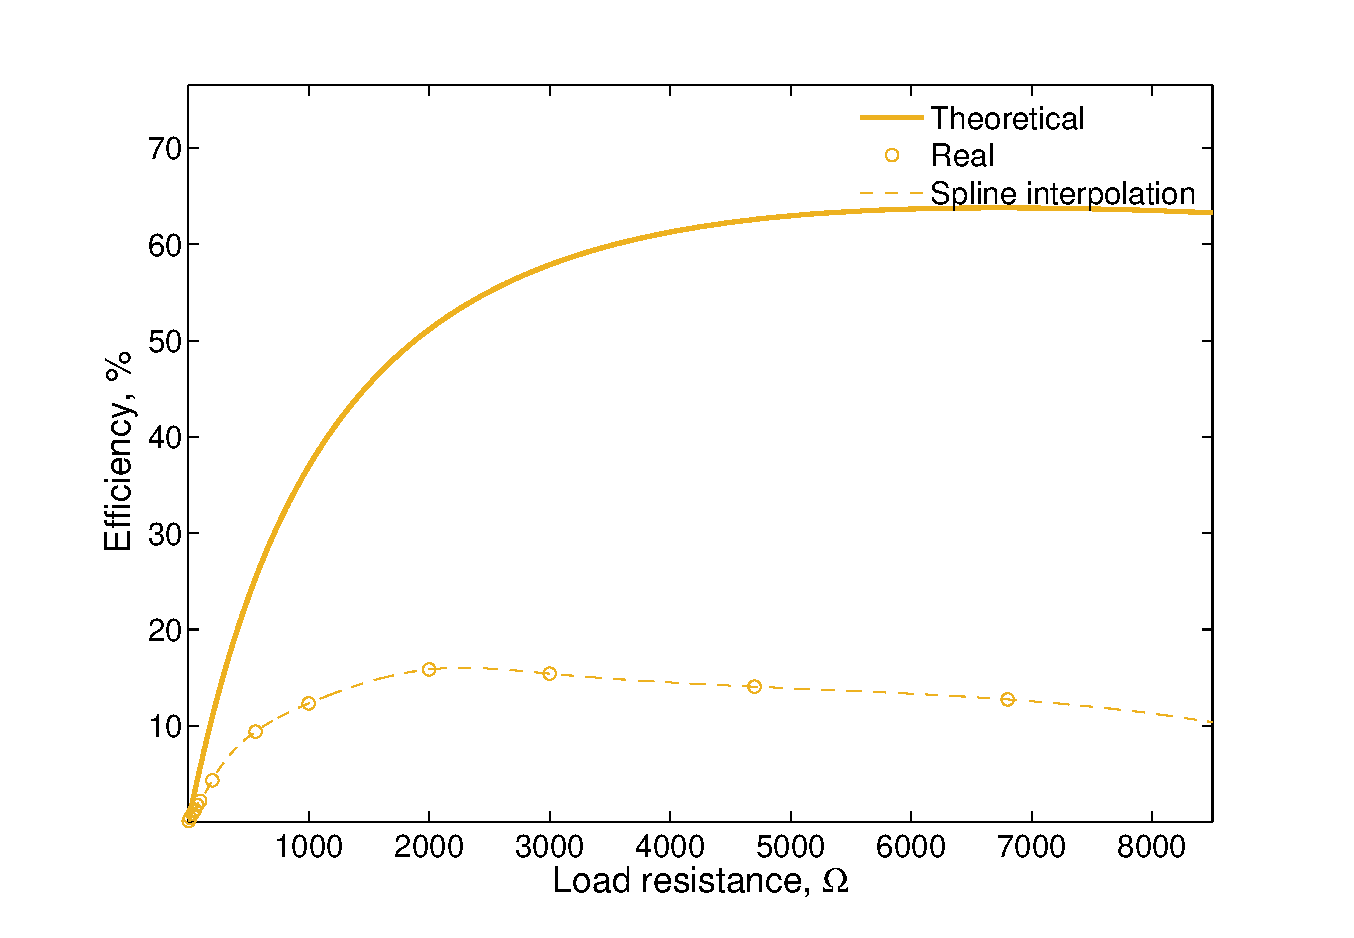
\includegraphics[width=0.5\textwidth]{./images/ModeloP_A_ZL_3_eff}}
\end{subfigmatrix}
\caption{Efficiency w.r.t. load resistance for SP topology}
\end{figure}

%%%%%%%%%%%%%%%%%%%%%%%%%%%%%%%%%%%%%%%%%%%%%%%%

\begin{figure}[h]
\centering
\begin{subfigmatrix}{2} 
\subfigure[f = 0.7 MHz]
{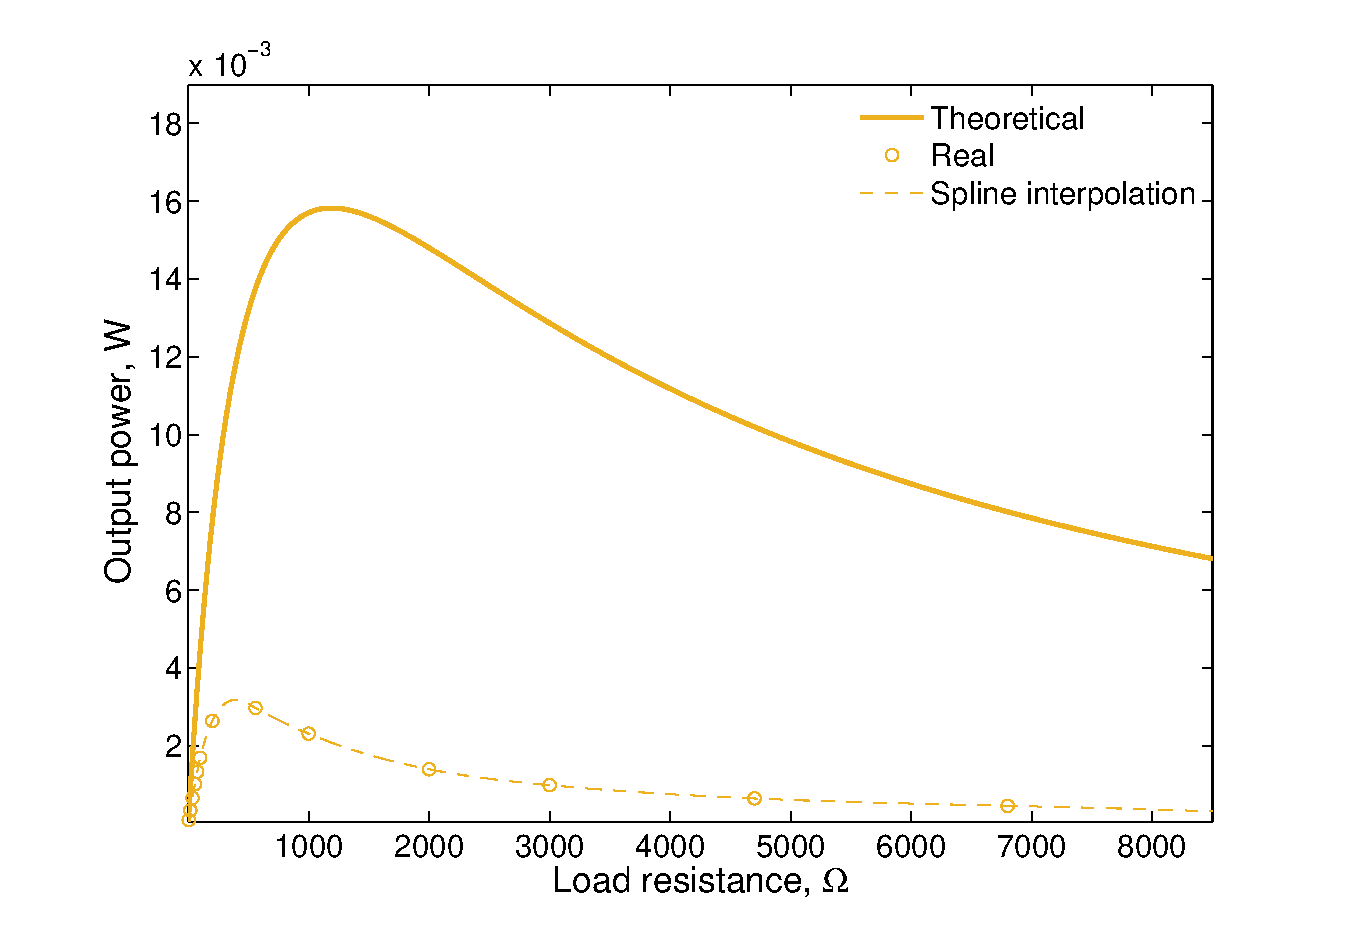
\includegraphics{./images/ModeloP_A_ZL_2_pout}}
\subfigure[f = 1 MHz]
{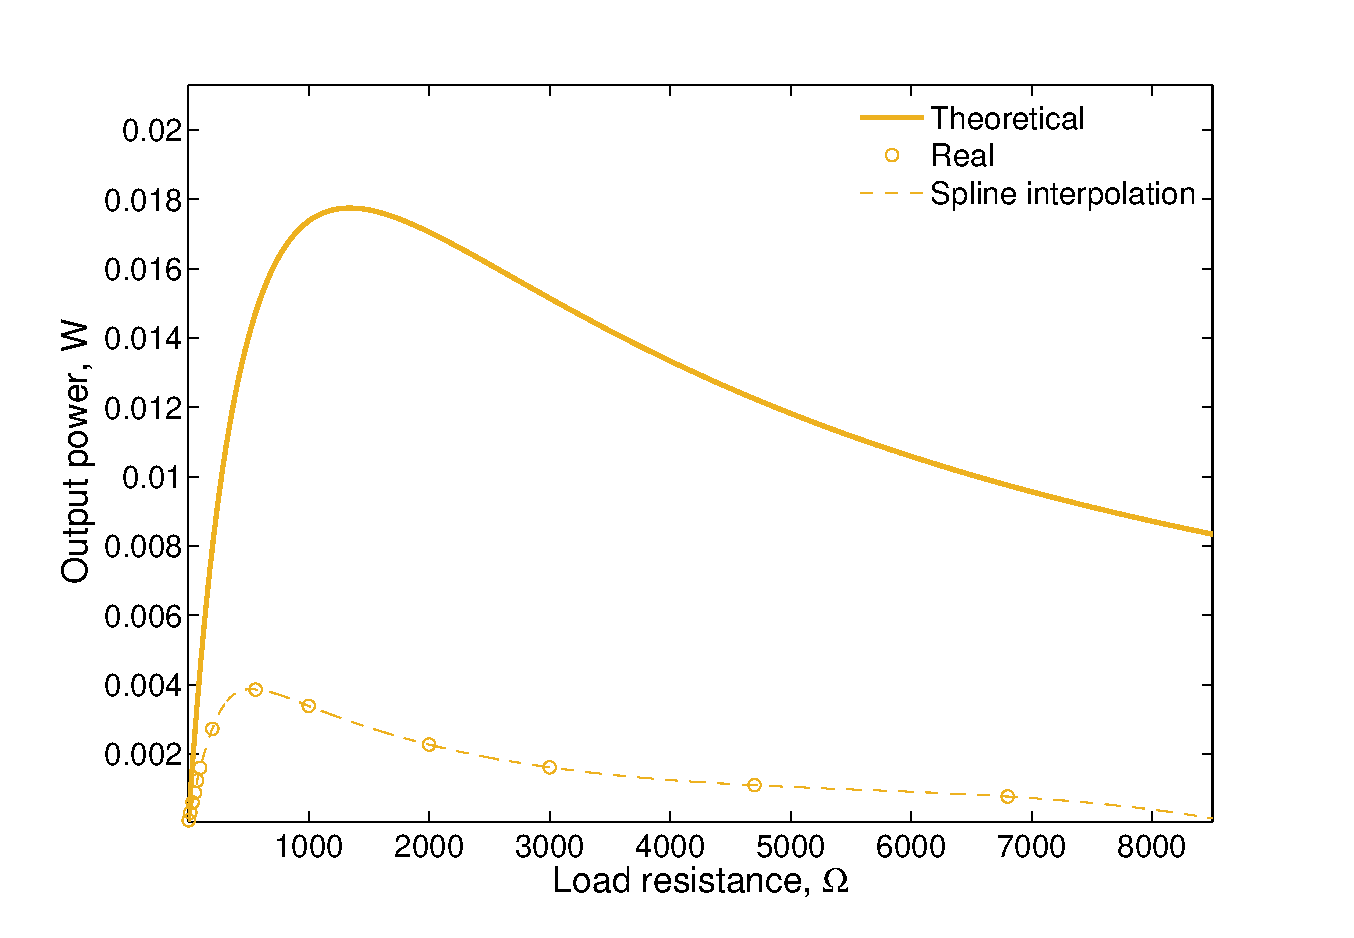
\includegraphics{./images/ModeloP_A_ZL_1_pout}}
\end{subfigmatrix}
\end{figure}
\begin{figure}[H]
\centering
\begin{subfigmatrix}{1} 
\subfigure[f = 2 MHz] 
{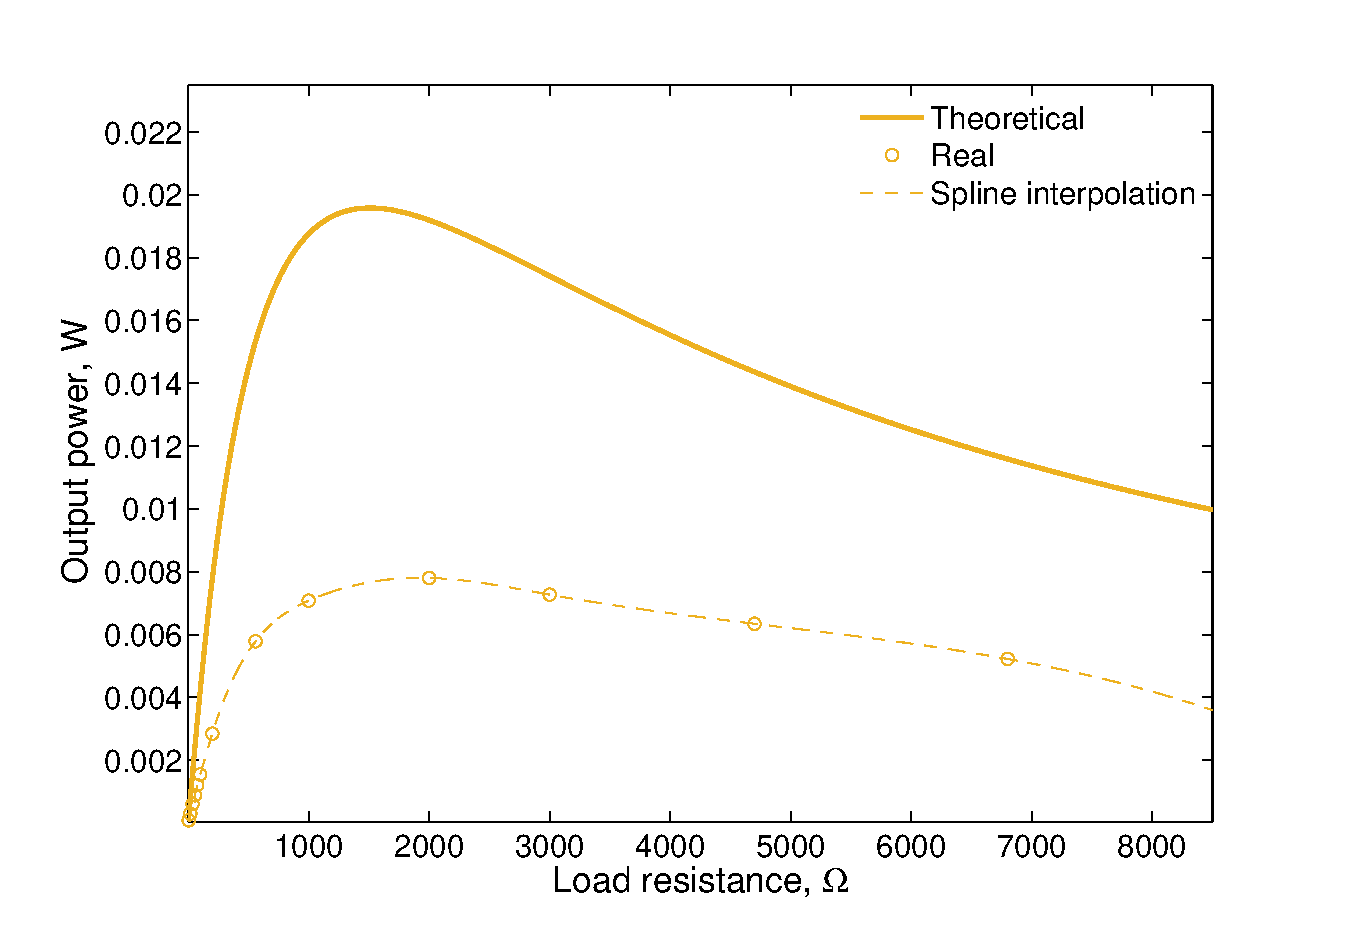
\includegraphics[width=0.5\textwidth]{./images/ModeloP_A_ZL_3_pout}}
\end{subfigmatrix}
\caption{Output power w.r.t. load resistance for SP topology}
\end{figure}

%%%%%%%%%%%%%%%%%%%%%%%%%%%%%%%%%%%%%%%%%%%%%%%%
%%%%%%%%%%%%%%%%%%%%%%%%%%%%%%%%%%%%%%%%%%%%%%%%
%%%%%%%%%%%%%%%%%%%%%%%%%%%%%%%%%%%%%%%%%%%%%%%%

\section{Model B}

\begin{figure}[h]
\centering
\begin{subfigmatrix}{2} 
\subfigure[f = 0.7 MHz]
{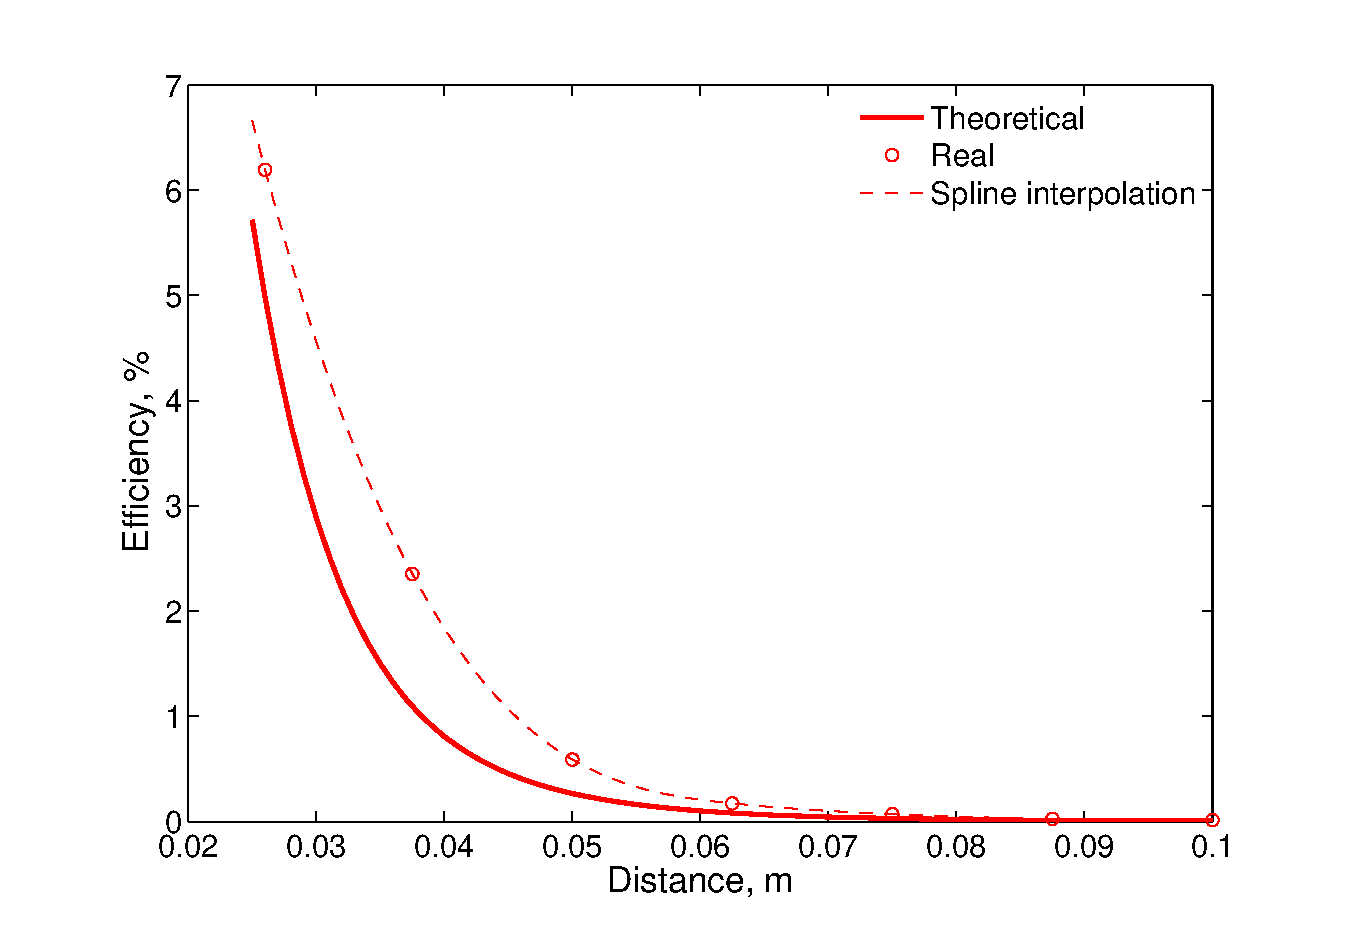
\includegraphics{./images/ModeloS_B_2_eff}}
\subfigure[f = 1 MHz]
{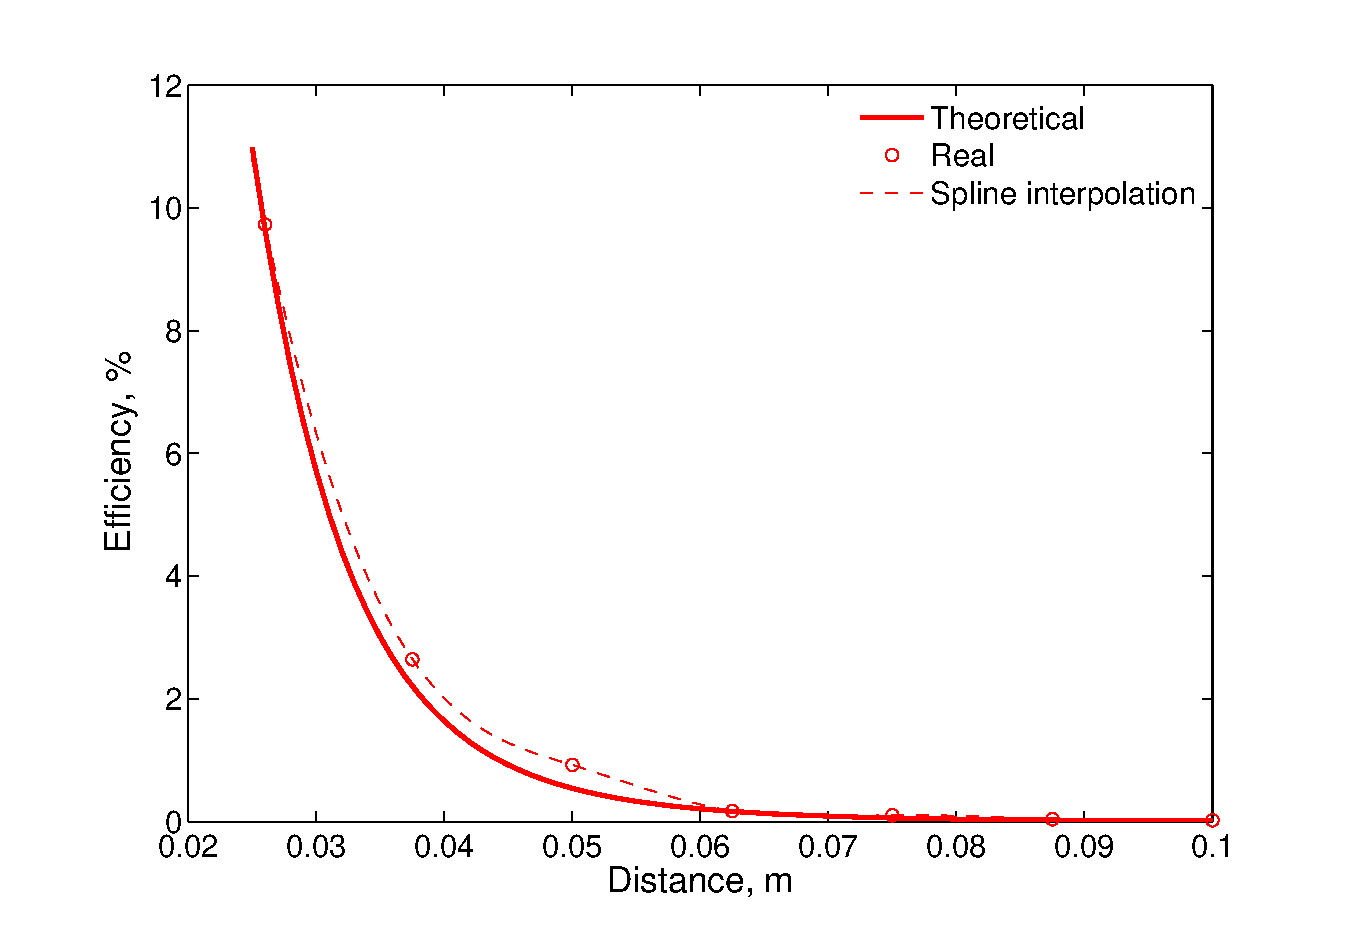
\includegraphics{./images/ModeloS_B_1_eff}}
\end{subfigmatrix}
\end{figure}
% \\[1pt]
\begin{figure}[H]
\centering
\begin{subfigmatrix}{1} 
\subfigure[f = 2 MHz] 
{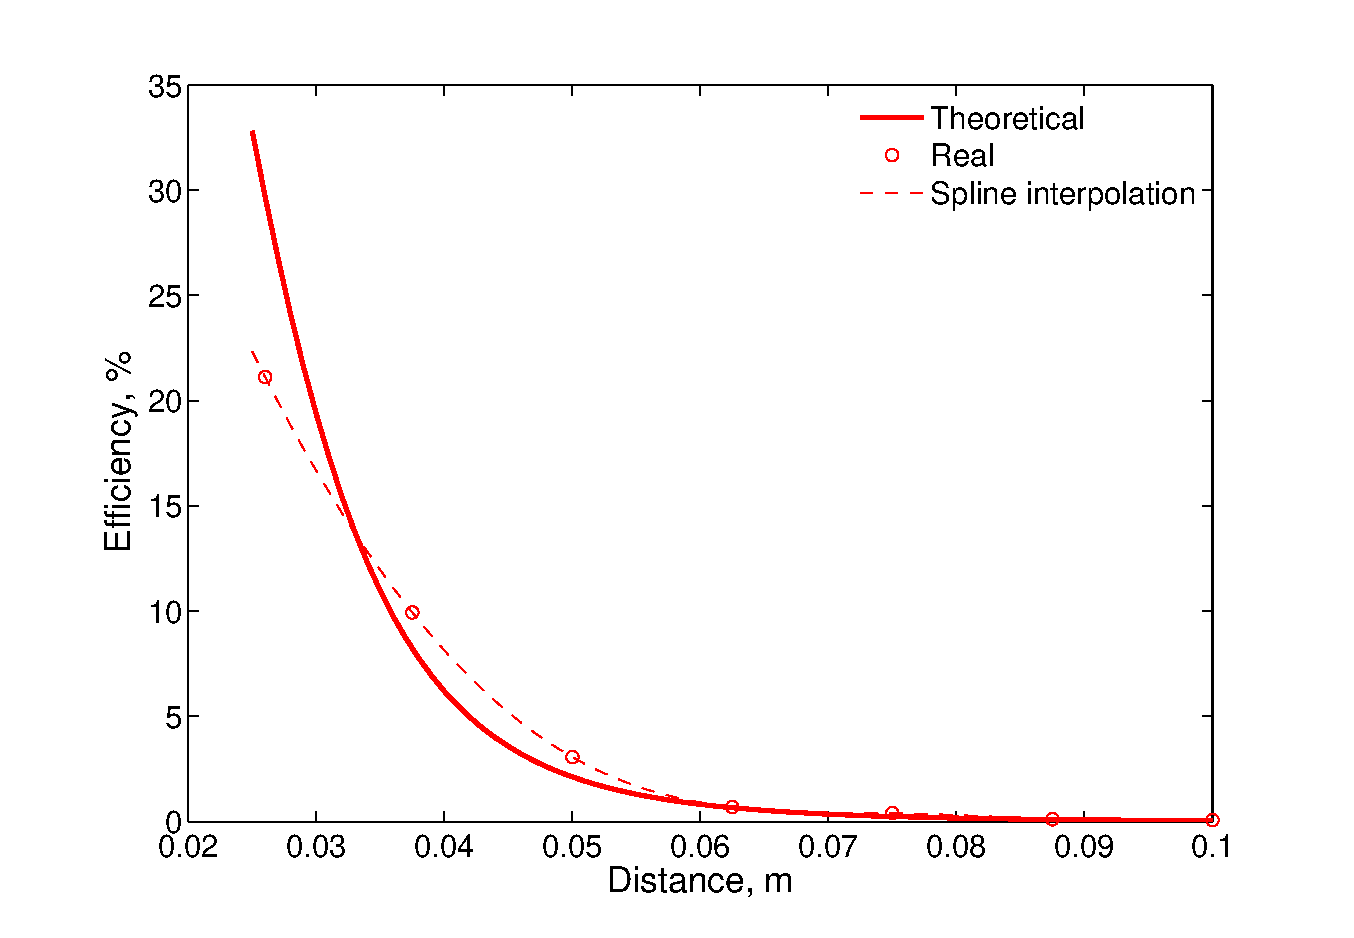
\includegraphics[width=0.5\textwidth]{./images/ModeloS_B_3_eff}}
\end{subfigmatrix}
\caption{Efficiency w.r.t. distance for SS topology}
\end{figure}

%%%%%%%%%%%%%%%%%%%%%%%%%%%%%%%%%%%%%%%%%%%%%%%%

\begin{figure}[h]
\centering
\begin{subfigmatrix}{2} 
\subfigure[f = 0.7 MHz]
{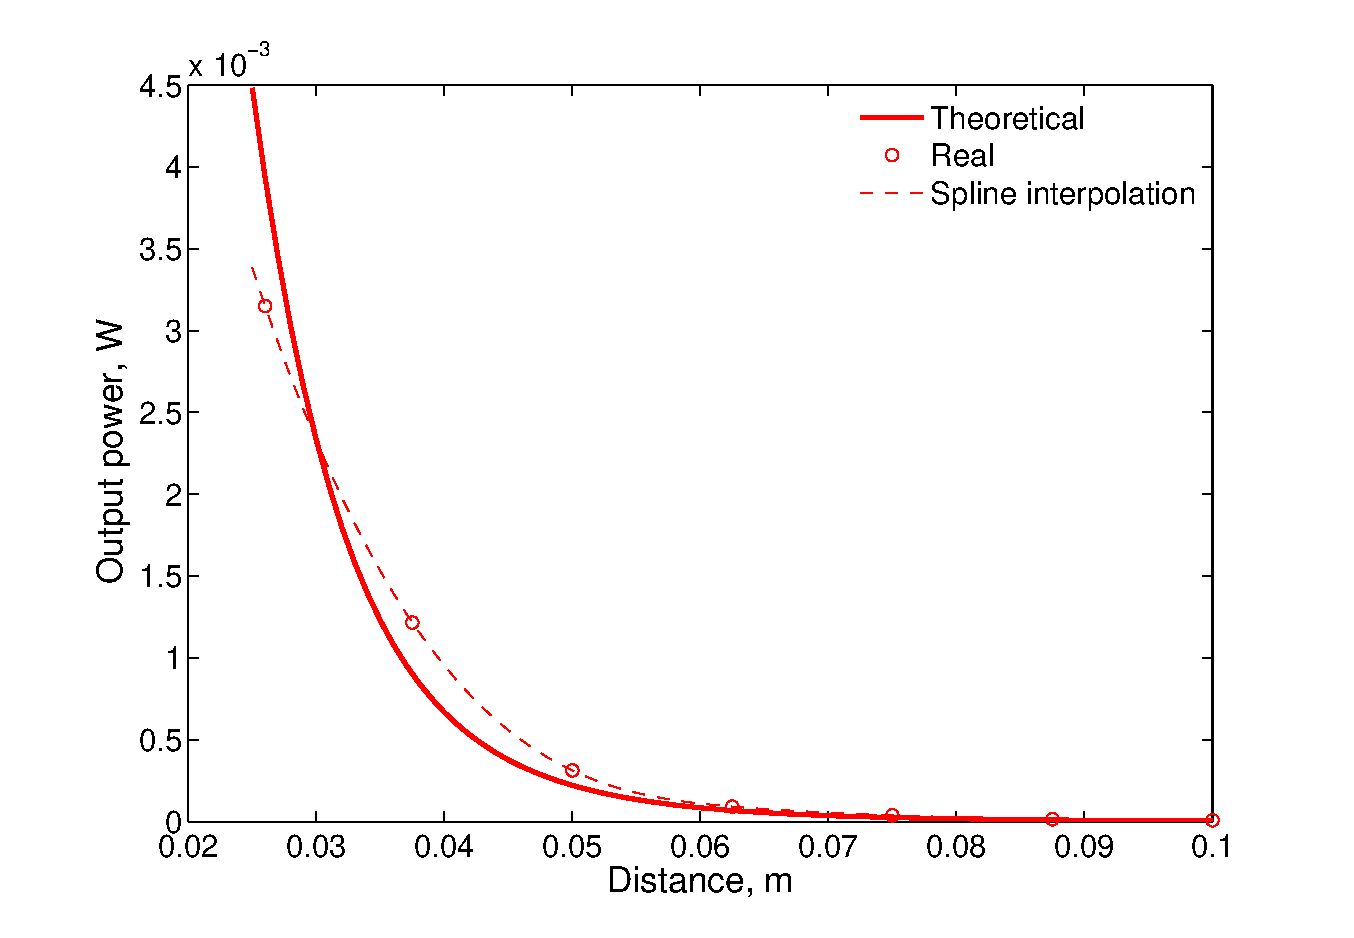
\includegraphics{./images/ModeloS_B_2_pout}}
\subfigure[f = 1 MHz]
{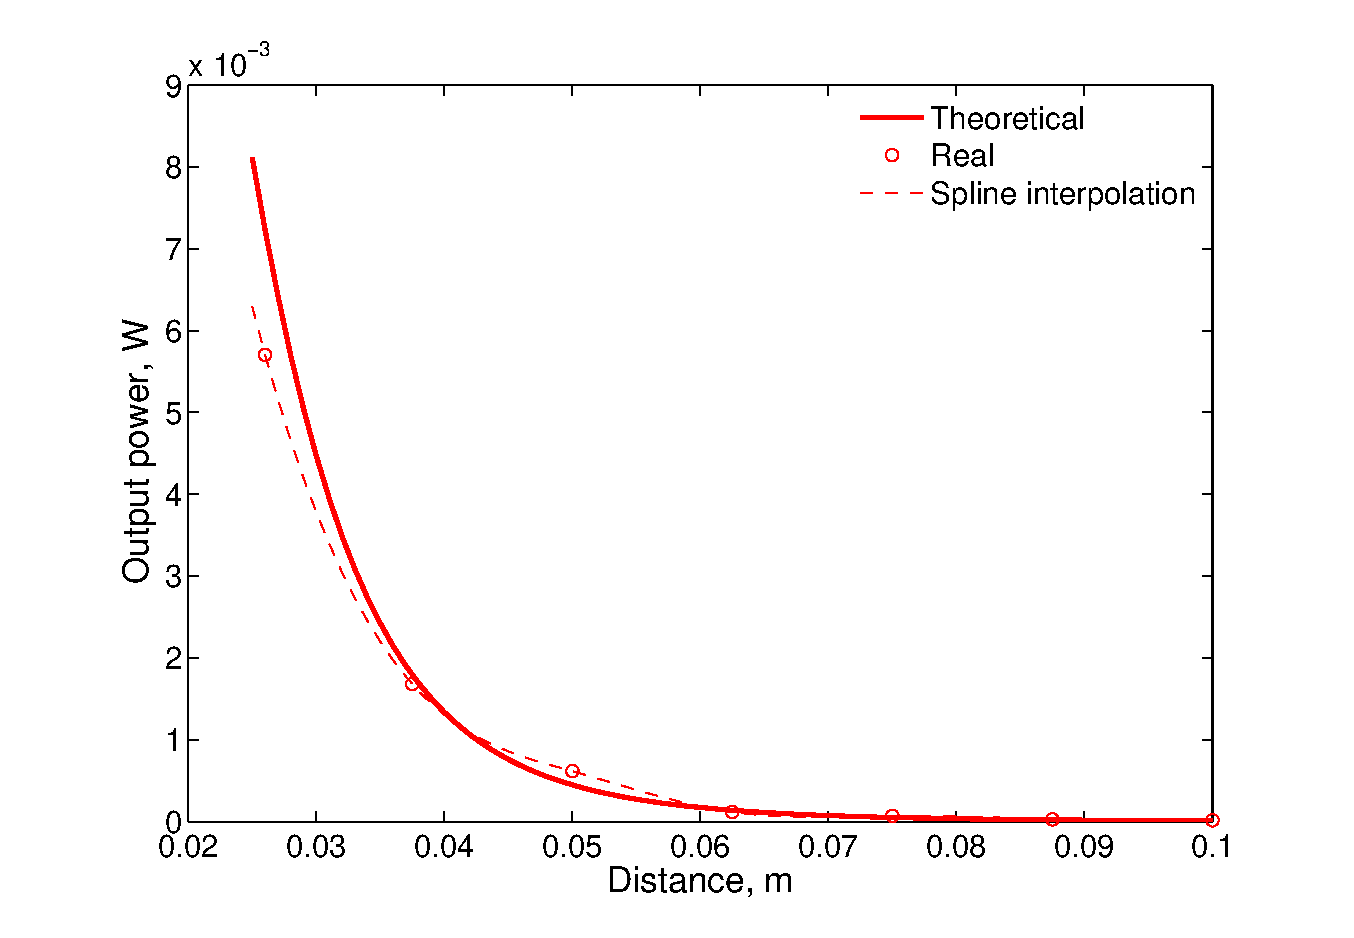
\includegraphics{./images/ModeloS_B_1_pout}}
\end{subfigmatrix}
\end{figure}
\begin{figure}[H]
\centering
\begin{subfigmatrix}{1} 
\subfigure[f = 2 MHz] 
{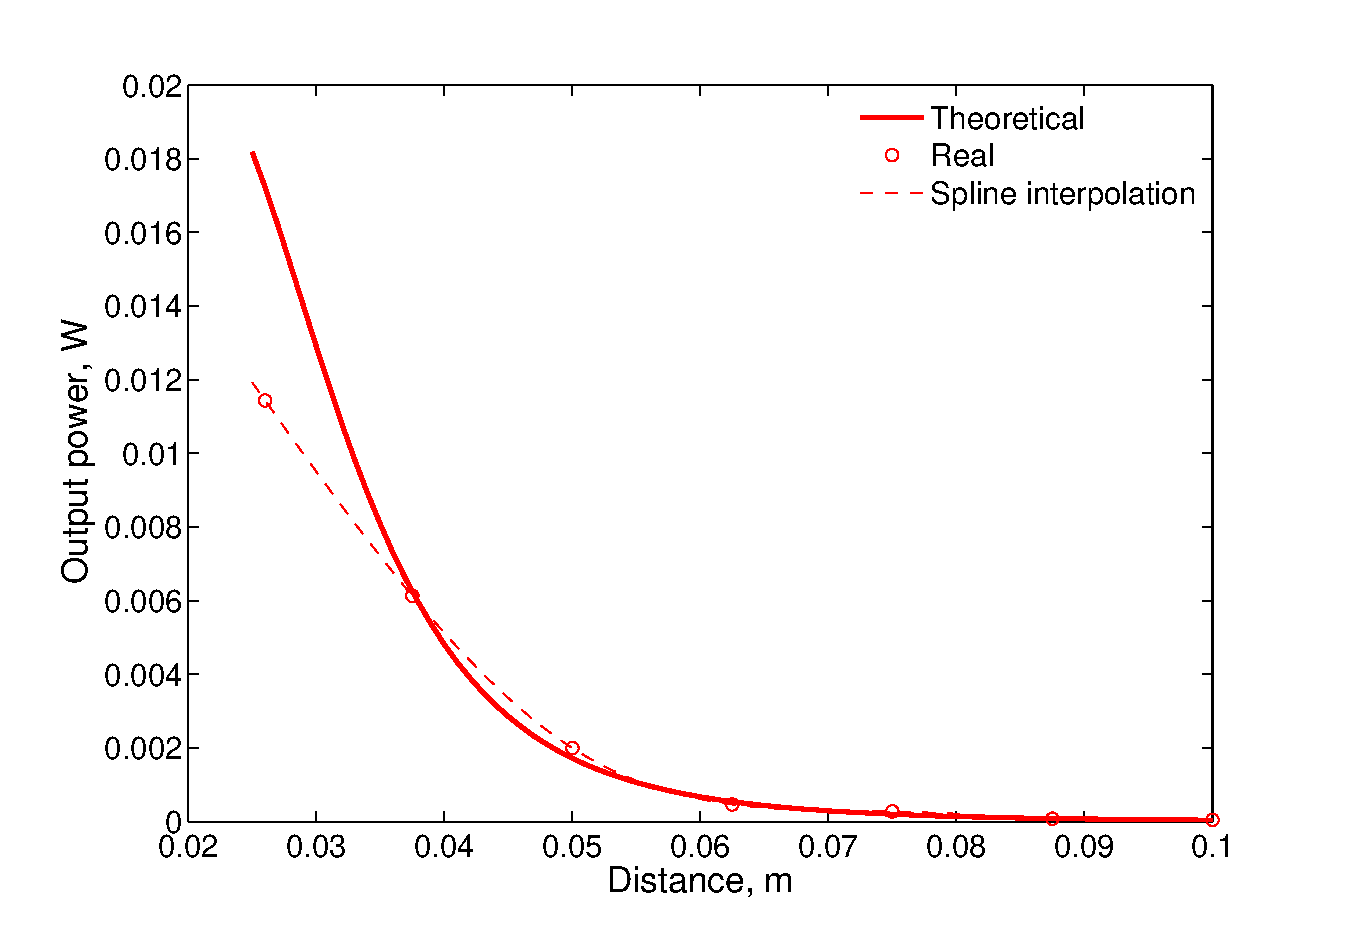
\includegraphics[width=0.5\textwidth]{./images/ModeloS_B_3_pout}}
\end{subfigmatrix}
\caption{Output power w.r.t. distance for SS topology}
\end{figure}

%%%%%%%%%%%%%%%%%%%%%%%%%%%%%%%%%%%%%%%%%%%%%%%%

\begin{figure}[h]
\centering
\begin{subfigmatrix}{2} 
\subfigure[f = 0.7 MHz]
{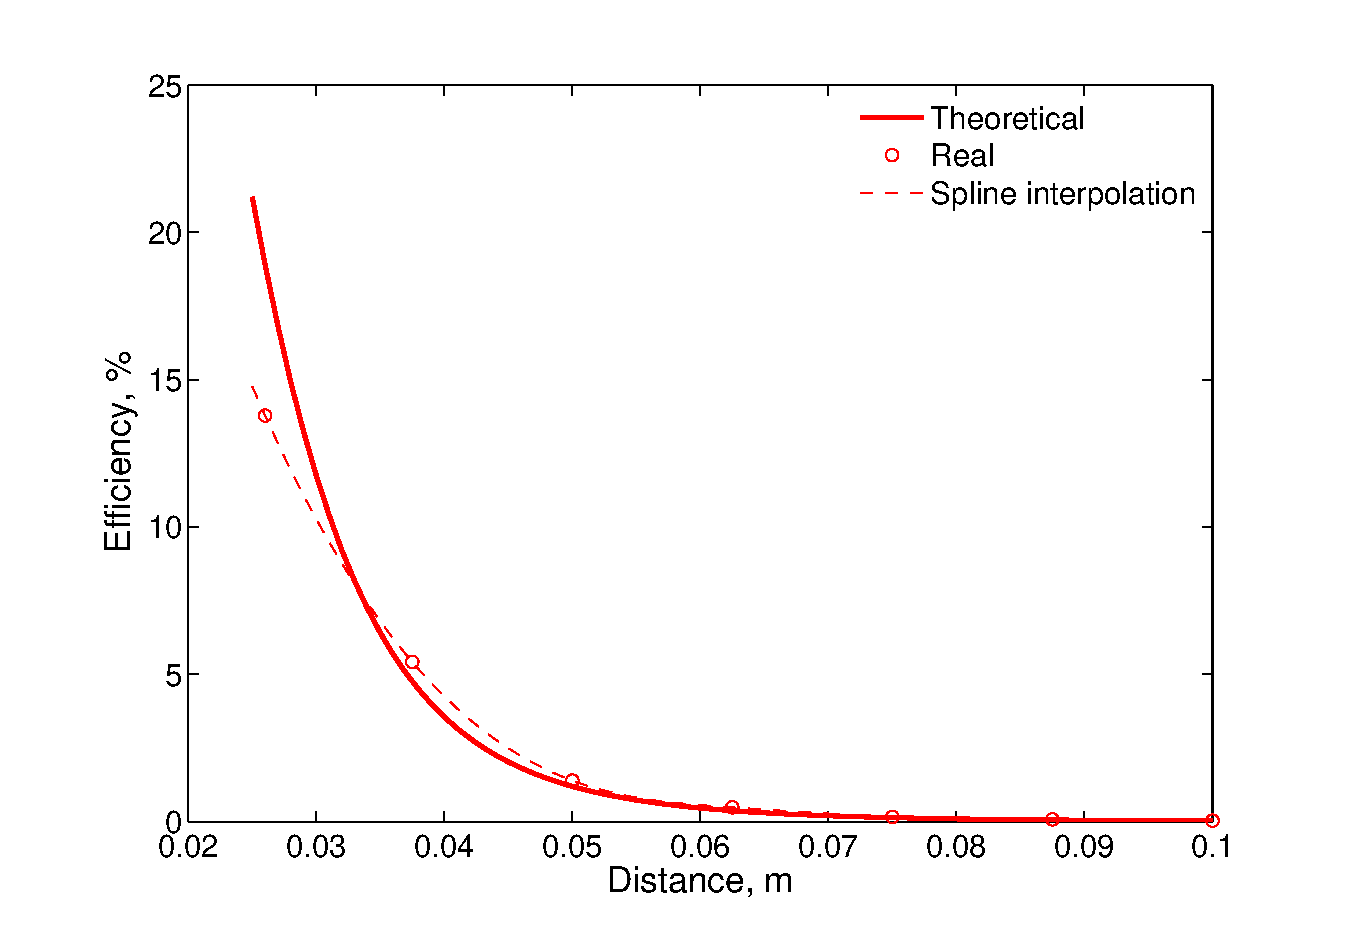
\includegraphics{./images/ModeloP_B_2_eff}}
\subfigure[f = 1 MHz]
{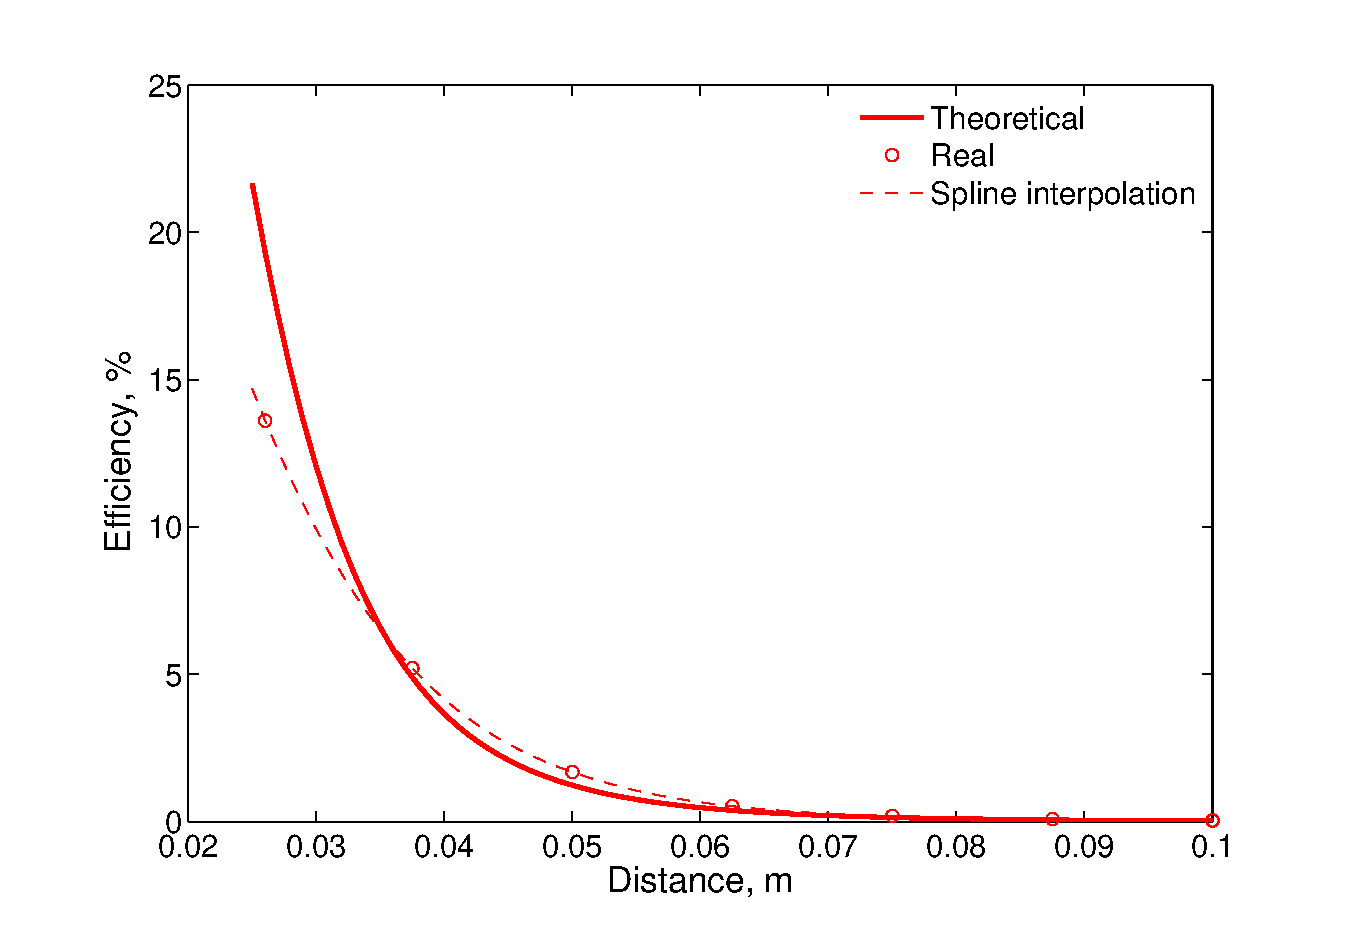
\includegraphics{./images/ModeloP_B_1_eff}}
\end{subfigmatrix}
\end{figure}
\begin{figure}[H]
\centering
\begin{subfigmatrix}{1} 
\subfigure[f = 2 MHz] 
{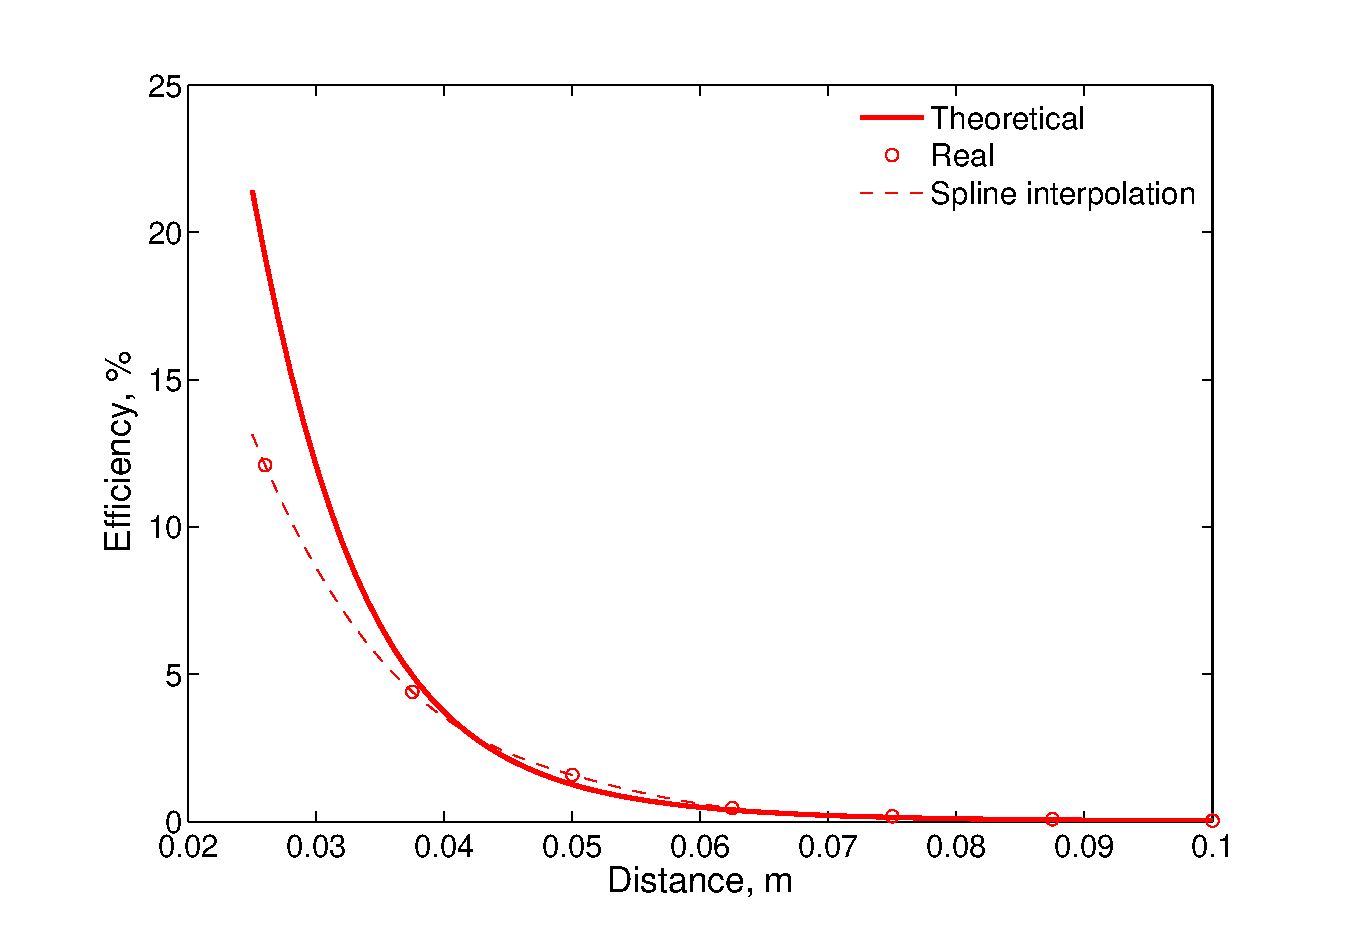
\includegraphics[width=0.5\textwidth]{./images/ModeloP_B_3_eff}}
\end{subfigmatrix}
\caption{Efficiency w.r.t. distance for SP topology}
\end{figure}

%%%%%%%%%%%%%%%%%%%%%%%%%%%%%%%%%%%%%%%%%%%%%%%%

\begin{figure}[h]
\centering
\begin{subfigmatrix}{2} 
\subfigure[f = 0.7 MHz]
{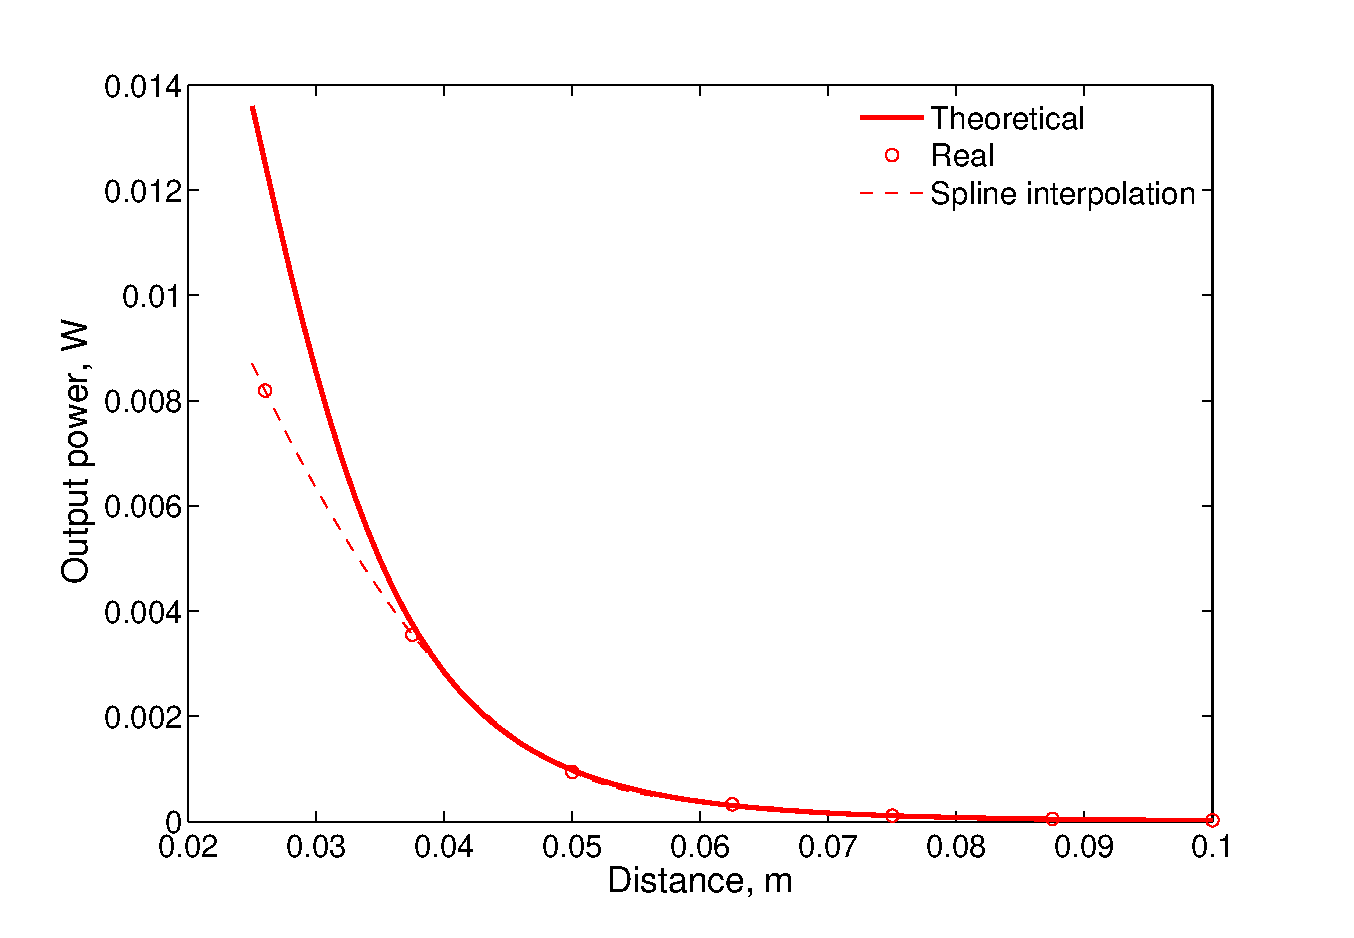
\includegraphics{./images/ModeloP_B_2_pout}}
\subfigure[f = 1 MHz]
{\includegraphics{./images/ModeloP_B_1_pout}}
\end{subfigmatrix}
\end{figure}
\begin{figure}[H]
\centering
\begin{subfigmatrix}{1} 
\subfigure[f = 2 MHz] 
{\includegraphics[width=0.5\textwidth]{./images/ModeloP_B_3_pout}}
\end{subfigmatrix}
\caption{Output power w.r.t. distance for SP topology}
\end{figure}

%%%%%%%%%%%%%%%%%%%%%%%%%%%%%%%%%%%%%%%%%%%%%%%%

\begin{figure}[h]
\centering
\begin{subfigmatrix}{2} 
\subfigure[f = 0.7 MHz]
{\includegraphics{./images/ModeloS_B_ZL_2_eff}}
\subfigure[f = 1 MHz]
{\includegraphics{./images/ModeloS_B_ZL_1_eff}}
\end{subfigmatrix}
\end{figure}
\begin{figure}[H]
\centering
\begin{subfigmatrix}{1} 
\subfigure[f = 2 MHz] 
{\includegraphics[width=0.5\textwidth]{./images/ModeloS_B_ZL_3_eff}}
\end{subfigmatrix}
\caption{Efficiency w.r.t. load resistance for SS topology}
\end{figure}

%%%%%%%%%%%%%%%%%%%%%%%%%%%%%%%%%%%%%%%%%%%%%%%%

\begin{figure}[h]
\centering
\begin{subfigmatrix}{2} 
\subfigure[f = 0.7 MHz]
{\includegraphics{./images/ModeloS_B_ZL_2_pout}}
\subfigure[f = 1 MHz]
{\includegraphics{./images/ModeloS_B_ZL_1_pout}}
\end{subfigmatrix}
\end{figure}
\begin{figure}[H]
\centering
\begin{subfigmatrix}{1} 
\subfigure[f = 2 MHz] 
{\includegraphics[width=0.5\textwidth]{./images/ModeloS_B_ZL_3_pout}}
\end{subfigmatrix}
\caption{Output power w.r.t. load resistance for SS topology}
\end{figure}

%%%%%%%%%%%%%%%%%%%%%%%%%%%%%%%%%%%%%%%%%%%%%%%%

\begin{figure}[h]
\centering
\begin{subfigmatrix}{2} 
\subfigure[f = 0.7 MHz]
{\includegraphics{./images/ModeloP_B_ZL_2_eff}}
\subfigure[f = 1 MHz]
{\includegraphics{./images/ModeloP_B_ZL_1_eff}}
\end{subfigmatrix}
\end{figure}
\begin{figure}[H]
\centering
\begin{subfigmatrix}{1} 
\subfigure[f = 2 MHz] 
{\includegraphics[width=0.5\textwidth]{./images/ModeloP_B_ZL_3_eff}}
\end{subfigmatrix}
\caption{Efficiency w.r.t. load resistance for SP topology}
\end{figure}

%%%%%%%%%%%%%%%%%%%%%%%%%%%%%%%%%%%%%%%%%%%%%%%%

\begin{figure}[h]
\centering
\begin{subfigmatrix}{2} 
\subfigure[f = 0.7 MHz]
{\includegraphics{./images/ModeloP_B_ZL_2_pout}}
\subfigure[f = 1 MHz]
{\includegraphics{./images/ModeloP_B_ZL_1_pout}}
\end{subfigmatrix}
\end{figure}
\begin{figure}[H]
\centering
\begin{subfigmatrix}{1} 
\subfigure[f = 2 MHz] 
{\includegraphics[width=0.5\textwidth]{./images/ModeloP_B_ZL_3_pout}}
\end{subfigmatrix}
\caption{Output power w.r.t. load resistance for SP topology}
\end{figure}

%%%%%%%%%%%%%%%%%%%%%%%%%%%%%%%%%%%%%%%%%%%%%%%%
%%%%%%%%%%%%%%%%%%%%%%%%%%%%%%%%%%%%%%%%%%%%%%%%
%%%%%%%%%%%%%%%%%%%%%%%%%%%%%%%%%%%%%%%%%%%%%%%%

\section{Model C}

\begin{figure}[h]
\centering
\begin{subfigmatrix}{2} 
\subfigure[f = 0.7 MHz]
{\includegraphics{./images/ModeloS_C_2_eff}}
\subfigure[f = 1 MHz]
{\includegraphics{./images/ModeloS_C_1_eff}}
\end{subfigmatrix}
\end{figure}
% \\[1pt]
\begin{figure}[H]
\centering
\begin{subfigmatrix}{1} 
\subfigure[f = 2 MHz] 
{\includegraphics[width=0.5\textwidth]{./images/ModeloS_C_3_eff}}
\end{subfigmatrix}
\caption{Efficiency w.r.t. distance for SS topology}
\end{figure}

%%%%%%%%%%%%%%%%%%%%%%%%%%%%%%%%%%%%%%%%%%%%%%%%

\begin{figure}[h]
\centering
\begin{subfigmatrix}{2} 
\subfigure[f = 0.7 MHz]
{\includegraphics{./images/ModeloS_C_2_pout}}
\subfigure[f = 1 MHz]
{\includegraphics{./images/ModeloS_C_1_pout}}
\end{subfigmatrix}
\end{figure}
\begin{figure}[H]
\centering
\begin{subfigmatrix}{1} 
\subfigure[f = 2 MHz] 
{\includegraphics[width=0.5\textwidth]{./images/ModeloS_C_3_pout}}
\end{subfigmatrix}
\caption{Output power w.r.t. distance for SS topology}
\end{figure}

%%%%%%%%%%%%%%%%%%%%%%%%%%%%%%%%%%%%%%%%%%%%%%%%

\begin{figure}[h]
\centering
\begin{subfigmatrix}{2} 
\subfigure[f = 0.7 MHz]
{\includegraphics{./images/ModeloP_C_2_eff}}
\subfigure[f = 1 MHz]
{\includegraphics{./images/ModeloP_C_1_eff}}
\end{subfigmatrix}
\end{figure}
\begin{figure}[H]
\centering
\begin{subfigmatrix}{1} 
\subfigure[f = 2 MHz] 
{\includegraphics[width=0.5\textwidth]{./images/ModeloP_C_3_eff}}
\end{subfigmatrix}
\caption{Efficiency w.r.t. distance for SP topology}
\end{figure}

%%%%%%%%%%%%%%%%%%%%%%%%%%%%%%%%%%%%%%%%%%%%%%%%

\begin{figure}[h]
\centering
\begin{subfigmatrix}{2} 
\subfigure[f = 0.7 MHz]
{\includegraphics{./images/ModeloP_C_2_pout}}
\subfigure[f = 1 MHz]
{\includegraphics{./images/ModeloP_C_1_pout}}
\end{subfigmatrix}
\end{figure}
\begin{figure}[H]
\centering
\begin{subfigmatrix}{1} 
\subfigure[f = 2 MHz] 
{\includegraphics[width=0.5\textwidth]{./images/ModeloP_C_3_pout}}
\end{subfigmatrix}
\caption{Output power w.r.t. distance for SP topology}
\end{figure}

%%%%%%%%%%%%%%%%%%%%%%%%%%%%%%%%%%%%%%%%%%%%%%%%
%%%%%%%%%%%%%%%%%%%%%%%%%%%%%%%%%%%%%%%%%%%%%%%%
\begin{figure}[h]
\centering
\begin{subfigmatrix}{2} 
\subfigure[f = 0.7 MHz]
{\includegraphics{./images/ModeloS_C_ZL_2_eff}}
\subfigure[f = 1 MHz]
{\includegraphics{./images/ModeloS_C_ZL_1_eff}}
\end{subfigmatrix}
\end{figure}
\begin{figure}[H]
\centering
\begin{subfigmatrix}{1} 
\subfigure[f = 2 MHz] 
{\includegraphics[width=0.5\textwidth]{./images/ModeloS_C_ZL_3_eff}}
\end{subfigmatrix}
\caption{Efficiency w.r.t. load resistance for SS topology}
\end{figure}

%%%%%%%%%%%%%%%%%%%%%%%%%%%%%%%%%%%%%%%%%%%%%%%%

\begin{figure}[h]
\centering
\begin{subfigmatrix}{2} 
\subfigure[f = 0.7 MHz]
{\includegraphics{./images/ModeloS_C_ZL_2_pout}}
\subfigure[f = 1 MHz]
{\includegraphics{./images/ModeloS_C_ZL_1_pout}}
\end{subfigmatrix}
\end{figure}
\begin{figure}[H]
\centering
\begin{subfigmatrix}{1} 
\subfigure[f = 2 MHz] 
{\includegraphics[width=0.5\textwidth]{./images/ModeloS_C_ZL_3_pout}}
\end{subfigmatrix}
\caption{Output power w.r.t. load resistance for SS topology}
\end{figure}

%%%%%%%%%%%%%%%%%%%%%%%%%%%%%%%%%%%%%%%%%%%%%%%%

\begin{figure}[h]
\centering
\begin{subfigmatrix}{2} 
\subfigure[f = 0.7 MHz]
{\includegraphics{./images/ModeloP_C_ZL_2_eff}}
\subfigure[f = 1 MHz]
{\includegraphics{./images/ModeloP_C_ZL_1_eff}}
\end{subfigmatrix}
\end{figure}
\begin{figure}[H]
\centering
\begin{subfigmatrix}{1} 
\subfigure[f = 2 MHz] 
{\includegraphics[width=0.5\textwidth]{./images/ModeloP_C_ZL_3_eff}}
\end{subfigmatrix}
\caption{Efficiency w.r.t. load resistance for SP topology}
\end{figure}

%%%%%%%%%%%%%%%%%%%%%%%%%%%%%%%%%%%%%%%%%%%%%%%%

\begin{figure}[h]
\centering
\begin{subfigmatrix}{2} 
\subfigure[f = 0.7 MHz]
{\includegraphics{./images/ModeloP_C_ZL_2_pout}}
\subfigure[f = 1 MHz]
{\includegraphics{./images/ModeloP_C_ZL_1_pout}}
\end{subfigmatrix}
\end{figure}
\begin{figure}[H]
\centering
\begin{subfigmatrix}{1} 
\subfigure[f = 2 MHz] 
{\includegraphics[width=0.5\textwidth]{./images/ModeloP_C_ZL_3_pout}}
\end{subfigmatrix}
\caption{Output power w.r.t. load resistance for SP topology}
\end{figure}

%%%%%%%%%%%%%%%%%%%%%%%%%%%%%%%%%%%%%%%%%%%%%%%%
%%%%%%%%%%%%%%%%%%%%%%%%%%%%%%%%%%%%%%%%%%%%%%%%
%%%%%%%%%%%%%%%%%%%%%%%%%%%%%%%%%%%%%%%%%%%%%%%%
\section{Output power for models D1 and D2}\label{D1D2}
This plots demonstrate that a bigger receiver coil diameter is preferred upon a bigger transmitter coil diameter. This is stated at Section \ref{subsec:geo}
\begin{figure}[H]
\centering
\begin{subfigmatrix}{2} 
\subfigure[D1 (Tx) / D2 (Rx)]
{\includegraphics{./images/D12}}
\subfigure[D2 (Tx) / D1 (Rx)]
{\includegraphics{./images/D21}}
\end{subfigmatrix}
\caption{Experimental demonstration of the output power depending on the coil receiver radius}
\end{figure}







\chapter{Programming Code}
Along this project, the plots and the mathematical model have been perfomed using \textit{MATLAB}. Some important codes are shown below. 


%% MATLAB example
% \begin{lstlisting}
% function y = myfun(aa, sigma, options)
% \end{lstlisting}

\lstinputlisting{./matlab/ExperimentalCoils.m}
\lstinputlisting{./matlab/FourTopologies.m}
\lstinputlisting{./matlab/SStopologyModel.m}
\lstinputlisting{./matlab/SPtopologyModel.m}
\lstinputlisting{./matlab/AC_Resistance.m}

\includepdf[pages={1}]{./images/MotorMount1.pdf}
\includepdf[pages={1}]{./images/BQ25504datasheet.pdf}
\includepdf[pages={2}]{./images/BQ25504datasheet.pdf}
\includepdf[pages={3}]{./images/BQ25504datasheet.pdf}
\includepdf[pages={4}]{./images/BQ25504datasheet.pdf}
\includepdf[pages={5}]{./images/slau227f.pdf}
\includepdf[pages={8}]{./images/slau227f.pdf}

